% This is a template for Ph.D. dissertations in the UCI format.
% 
% All fonts, including those for sub- and superscripts, must be 10
% points or larger.  Recommended sizes are 14-point for chapter
% headings, 12-point for the main body of text and figure/table
% titles, and 10-point for footnotes, sub- and super-scripts, and text
% in figures and tables.
%
% Notes: Add short title to figures, sections, via square brackets,
% e.g. \section[short]{long}.
%
\documentclass[12pt,fleqn]{ucithesis}

% A few common packages

\usepackage{amsmath}
\usepackage{amsthm}
\usepackage{array}
\usepackage{graphicx}
\usepackage{natbib}
\usepackage{relsize}
\usepackage{subfigure}
\usepackage{graphicx}
% Some other useful packages
\usepackage{caption}
%\usepackage{subcaption} %\begin{subfigure}...\end{subfigure} within figure
\usepackage{multirow}
\usepackage{tabularx}

% plainpages=false fixes the "duplicate ignored" error with page counters
% Set pdfborder to 0 0 0 to disable colored borders around PDF hyperlinks
\usepackage[plainpages=false,pdfborder={0 0 0}]{hyperref}

% Uncomment the following two lines to use the algorithm package,
% which provides an algorithm environment similar to figure and table
% ("\begin{algorithm}...\end{algorithm}"). A list of algorithms will
% automatically be added in the preliminary pages. Note that you
% probably want a package for the actual code to go with this (e.g.,
% algorithmic).
%\usepackage{algorithm}
%\renewcommand{\listalgorithmname}{\protect\centering\protect\Large LIST OF ALGORITHMS}

% Uncomment the following line to enable Unicode support. This will allow you
% to enter non-ASCII characters (such as accented characters) directly without
% having to use LaTeX's awkward escape syntax (e.g., \'{e})
% NOTE: You may have to install the ucs.sty package for this to work. See:
% http://www.unruh.de/DniQ/latex/unicode/
%\usepackage[utf8x]{inputenc}

% Uncomment the following to avoid "widowing", where page breaks cause
% single lines of paragraphs to float onto the next page (this is not
% a UCI requirement but more of an aesthetic choice).
\widowpenalty=10000
\clubpenalty=10000

% Modify or extend these at will.
\newtheorem{theorem}{\textsc{Theorem}}[chapter]
\newtheorem{definition}{\textsc{Definition}}[chapter]
\newtheorem{example}{\textsc{Example}}[chapter]

% Macros for title, author, abstract, etc.
\thesistitle{Spin torque driven magnetization dynamics in nanoscale magnetic tunnel junctions}

%"Dissertation" for PhD, "Thesis" for master's
\documenttitle{Dissertation}

\degreename{Doctor of Philosophy}

% Use the wording given in the official list of degrees awarded by UCI:
% http://www.rgs.uci.edu/grad/academic/degrees_offered.htm
\degreefield{Physics}

% Your name as it appears on official UCI records.
\authorname{Chengcen Sha}

% Use the full name of each committee member.
\committeechair{Professor Ilya Krivorotov}
\othercommitteemembers
{
  Professor Wilson Ho\\
  Professor Jing Xia
}

\degreeyear{2018}

\copyrightdeclaration
{
  {\copyright} {\Degreeyear} \Authorname
}

% If you have previously published parts of your manuscript, you must list the
% copyright holders; see Section 3.2 of the UCI Thesis and Dissertation Manual.
% Otherwise, this section may be omitted.
% \prepublishedcopyrightdeclaration
% {
% 	Chapter 4 {\copyright} 2003 Springer-Verlag \\
% 	Portion of Chapter 5 {\copyright} 1999 John Wiley \& Sons, Inc. \\
% 	All other materials {\copyright} {\Degreeyear} \Authorname
% }

% The dedication page is optional
% (comment out to exclude).
\dedications
{
  To My parents, Zhenglian and Wenyu.
}

\acknowledgments
{
  I would like to express my deepest appreciation to Professor Ilya Krivorotov. It is quite a privilege to work with him. I really learned a lot from his great knowledge of physics and sharp insights into problem solving. I still remember almost six years ago I had my first Skype interview with Ilya and he asked me about exchange bias effect. Without his guidance and help this dissertation would not be possible.
  
  I would also like to thank all my lab mates : Zheng Duan, Igor Barsukov, Eric Montoya, Brian Youngblood, Yu-Jin Chen, Andrew  Smith,  Han Kyu Lee, Jenru Chen, Jieyi Zhang,  Alejandro Jara, Chris Safranski and Josh Dill. I have been received a great amount of help since the first day I joined the lab. When I first joined the lab, I did not know even most simple thing, such as using a torque wrench and basis soldering. These guys helped me overcome a lot of difficulties and provided help whenever I asked. I never wished I could be surrounded by such a amazing group of people and I really feel honored to call these guys my lab mate.
  
  During the last five years in the United States, I am happy to keep in touch with my good friends over the world. I would like to thank Jiao Li, Rui Da, Ruohui Yang, Xun Liu, Hongyu Zhu and Qingyu Zhu. Those people are all pursuing or have already obtained their Ph.D. degree and we have had lots of useful/useless discussions about our common experiences. We shared numerous joy and distress over the past five years. I might not be able to see these friends quite often and in fact, I have not met some of them for almost five years. However, their support is greatly valuable to me and I really hope nothing but the best for all of them from my heart.
  
  Of course I am extremely luck to have a loving family. My parents have been the greatest support to me without any conditions. They have provided all they can give to me and I cannot pay back them enough. My wife has been the angle of my life and I love her very much. Of course I cannot forget my cat Luca, who gives me lots of joy when I was lonely.
  
}


% Some custom commands for your list of publications and software.
\newcommand{\mypubentry}[3]{
  \begin{tabular*}{1\textwidth}{@{\extracolsep{\fill}}p{4.5in}r}
    \textbf{#1} & \textbf{#2} \\ 
    \multicolumn{2}{@{\extracolsep{\fill}}p{.95\textwidth}}{#3}\vspace{6pt} \\
  \end{tabular*}
}
\newcommand{\mysoftentry}[3]{
  \begin{tabular*}{1\textwidth}{@{\extracolsep{\fill}}lr}
    \textbf{#1} & \url{#2} \\
    \multicolumn{2}{@{\extracolsep{\fill}}p{.95\textwidth}}
    {\emph{#3}}\vspace{-6pt} \\
  \end{tabular*}
}

% Include, at minimum, a listing of your degrees and educational
% achievements with dates and the school where the degrees were
% earned. This should include the degree currently being
% attained. Other than that it's mostly up to you what to include here
% and how to format it, below is just an example.
%
% CV is required for PhD theses, but not Master's
% comment out to exclude

\curriculumvitae
{

\textbf{EDUCATION}
  
  \begin{tabular*}{1\textwidth}{@{\extracolsep{\fill}}lr}
    \textbf{Doctor of Philosophy in Physics} & \textbf{2018} \\
    \vspace{6pt}
    University of California Irvine & \emph{Irvine, CA, United States} \\
    \textbf{Bachelor of Science} & \textbf{2013} \\
    \vspace{6pt}
    Nanjing University & \emph{Nanjing, China} \\
  \end{tabular*}

\vspace{12pt}
\textbf{RESEARCH EXPERIENCE}

  \begin{tabular*}{1\textwidth}{@{\extracolsep{\fill}}lr}
    \textbf{Graduate Research Assistant} & \textbf{2013--2018} \\
    \vspace{6pt}
    University of California, Irvine & \emph{Irvine, California} \\
  \end{tabular*}

\vspace{12pt}
\textbf{TEACHING EXPERIENCE}

  \begin{tabular*}{1\textwidth}{@{\extracolsep{\fill}}lr}
    \textbf{Teaching Assistant} & \textbf{2013--2014} \\
    \vspace{6pt}
    University of California, Irvine & \emph{Irvine, California} \\
  \end{tabular*}



\vspace{12pt}
\textbf{SELECTED PRESENTATIONS AND POSTERS }

	\mypubentry{Characterization of perpendicular STT-MRAM by ST-FMR}{March 2016}{APS March Meeting}
  \mypubentry{Ferromagnetic Resonance Linewidth in Nanoscale Magnetic Tunnel Junctions }{November 2017}{MMM}
  \mypubentry{Ferromagnetic resonance linewidth in nanoscale magnetic tunnel junctions }{August 2018}{International Conference on Magnetism}
  
}

% The abstract should not be over 350 words, although that's
% supposedly somewhat of a soft constraint.
\thesisabstract
{
 	Spin transfer torque is generated by the transfer of angular momentum from spin polarized electrons to a ferromagnet. This spin transfer torque provides an efficient way to manipulate the dynamic motion of the magnetization of a nanomagnet, and can be strong enough to induce magnetization switching and steady-state precession. This field of study draws enormous attention not only because spin transfer torque is essential in understanding fundamental physical phenomena, but also it makes the building block for future applications such as spin torque oscillators, magnetic random access memory.We have developed several new techniques to characterize such dynamics in nanoscale magnetic tunnel junctions. In this thesis we will first introduce a effect methods to characterize important material parameters in nano-scale Magnetic Tunnel Junctions: Spin-torque ferromagnetic resonance. This methods combing with micromagnetic modeling allows us to determine the magnetic anisotropy, Gilbert damping, exchange stiffness and shape distortion and damages. We will also demonstrate a single-shot electrical technique to capture the magnetic dynamics during the spin torque switching of a magnetic tunnel junction in real time. We also discuss measurement of switching probability of magnetic tunnel junctions by applying electric pulses.
}


%%% Local Variables: ***
%%% mode: latex ***
%%% TeX-master: "thesis.tex" ***
%%% End: ***


% Add PDF document info fields
\hypersetup{
	pdftitle={\Thesistitle},
	pdfauthor={\Authorname},
	pdfsubject={\Degreefield},
}

% Uncomment the following to have numbered subsubsections (by default
% numbering goes only to subsections).
%\setcounter{secnumdepth}{4}


% Set this to only select a subset of the includes directives below.
% Very handy to speed up compilation if you're working on a certain
% part of your thesis. It conserves page numbers, references, etc.
% even for non-included files.
%\includeonly{chapter1}

\begin{document}

% Preliminary pages are always loaded (TOC, CV, etc.)

\preliminarypages

% Include the different components of your thesis, in separate files.
% Using \include allows you to set \includeonly above.
%\chapter{Introduction}

  Spin transfer torque is generated by the transfer of angular momentum from spin polarized electrons to a ferromagnet. This spin transfer torque provides an efficient way to manipulate the dynamic motion of the magnetization of a nanomagnet, and can be strong enough to induce magnetization switching and steady-state precession. This field of study draws enormous attention not only because spin transfer torque is essential in understanding fundamental physical phenomena, but also it makes the building block for future applications such as spin torque oscillators, magnetic random access memory.We have developed several new techniques to characterize such dynamics in nanoscale magnetic tunnel junctions.
  
  In chapter 2, we will first discuss necessary background  knowledge in this field. In chapter 3, we develop a new reliable methods to characterize material parameters such as magnetic anisotropy and Gilbert damping using spin-torque ferromagnetic magnetic resonance with field-modulation. By performing micromagnetic simulations, we can determine other spatial-dependent parameters.
  
  In chapter 4, we demonstrate a single-shot electrical technique to capture the magnetic dynamics during the spin torque switching of a magnetic tunnel junction in real time. With improved sensitivity, we can directly observe real-time oscillation before switching.
  
  In chapter 5, we focus on measurement of switching probability of magnetic tunnel junctions by applying electric pulses. We observe anomalous write error rate behavior in our magnetic tunnel junctions samples. Possible origins of this anomalous write error rate has been discussed.


%%% Local Variables: ***
%%% mode: latex ***
%%% TeX-master: "thesis.tex" ***
%%% End: ***

%\chapter{Background}

\section{Spintronics}

Nearly five thousand years ago, people already discovered the natural magnets and they found out that when you move two magnets closer to each other, they can either be attractive or repulsive depending on the relative directions. Without understanding the mechanism, people already made some useful stuff such as a horseshoe magnet\cite{wiki:Ferromagnetism}.

\begin{figure}[!ht]
\centering
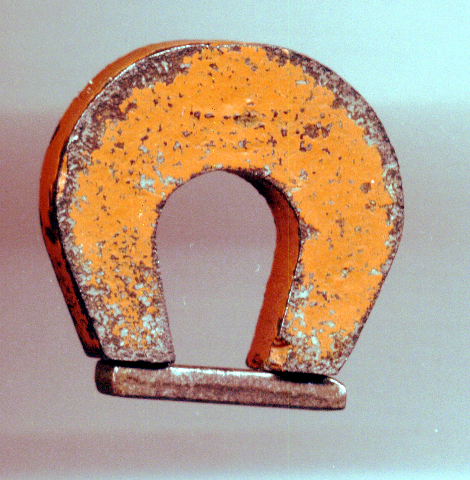
\includegraphics[width=0.3\textwidth]{fig/Magnet.jpg}
\label{Magnet}
\caption{A magnet made of alnico, an iron alloy, with its keeper.}
\end{figure}

However, it was not until 1925 that the underlying mystery of ferromagntism started to reveal itself. George Uhlenbeck and Samuel Goudsmit proposed the idea that each electron spins with an angular momentum of one half Planck constant and carries a magnetic moment of one Bohr magneton. Even though the famous Hendrik Lorentz pointed out that the idea of a spinning electron would be incompatible with classical electrodynamics, those two physicists went ahead and published their results. Of course, they were right and Lorentz was wrong. Uhlenbeck and Goudsmit maybe could not image their findings to have such a great impact on modern information technology. While electronics, the manipulations of electron charges in various kinds of devices, has been developed greatly since 1950s and shaped a new world, the development of spintronics started to influence the modern technology since 1980s. Johnson and Silsbee\cite{JohnsonandSilsbee} observed spin-polarized electron injection from a ferromagnetic metal to a normal metal.  Albert Fert\cite{Fert} and Peter Gr\"unberg\cite{Grunberg} independently discovered the phenomena of Giant magnetoresistance(GMR) and they have been rewarded The Nobel Prize in Physics 2007 for the practise significance of this work. Spintronics have several major advantages over conventional electronics. Unlike the conventional electronics which relies on the transportation of electrons charges, which inevitably creates heating dissipation and power loss, spintronics can perform with pure spin currents and movements of spin angular momentum without heat. Moreover, once formed, the spins does not need energy to maintain it. The non-volatility takes a huge advantages in static power consumption. Spintronics has a great ongoing and potential applications in memory storage, signal processing and logical devices.

\section{Tunnel Magnetoresistance}

The Tunnel Magnetoresistance effect\cite{TMR} refers to the change of resistance of a ferromagnetic/non-magnetic barrier/ferromagnetic metallic multilayer structure as the relative orientation of the magnetizations of two ferromagnetic layers changes. When the two layers have parallel magnetizations, the resistance is lowest and the resistance is maximum when magnetizations of two ferromagnetic layers are anti-parallel. Nowadays, the resistance difference between the maximum and minimum values can be as much as 100 per cent.

We first consider a simple case when electrons are passing through a single ferromagnetic layer. For a 3d transitional ferromagnetic layer like Ni, Co and Fe, ferromagnetism is coming from the exchange coupling of 3d electrons. In a simplified band structure for ferromagnetic metals, the exchange coupling results in an split of energy band for 3d electrons. As a result when the spin-up band and spin-down band are filled up to the Fermi level, there will be more spin-up electrons than spin-down electrons, which induces a net magnetization. On the other hand, the majority and minority spin bands also have different density of states at the Fermi level. The conduction properties of a metal are primarily determined by the electrons near the Fermi level. When spin unpolarized electrons consisting of equal numbers of spin-up and spin-down electrons travel in a ferromagnet, different spins experiences different resistances. Besides, different types of spins also experience different scattering at the interface due to the band structure mismatch. Overall, one type of spins has higher probability to transmit through than the other type.

\begin{figure}[!ht]
\centering
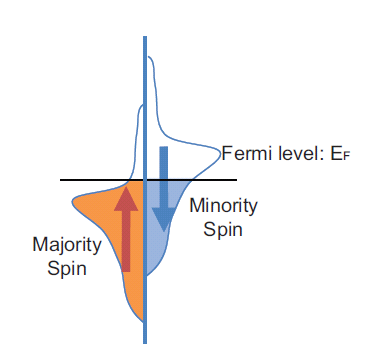
\includegraphics{fig/Fermi.PNG}
\label{Fermi}
\caption{Band structure for ferromagnet. Due to energy split, the majority and minority spin bands have different of states at the Fermi level.}

\end{figure}




Now, we have two magnetic layers separated by a tunnel barrier. As it has been proposed by Julliere in 1975, the tunneling probability across the tunnel barrier,which can be treated as conductance in this case, is proportional to the density of states of both initial and final states. Then we have 




\begin{figure}[!ht]
\centering
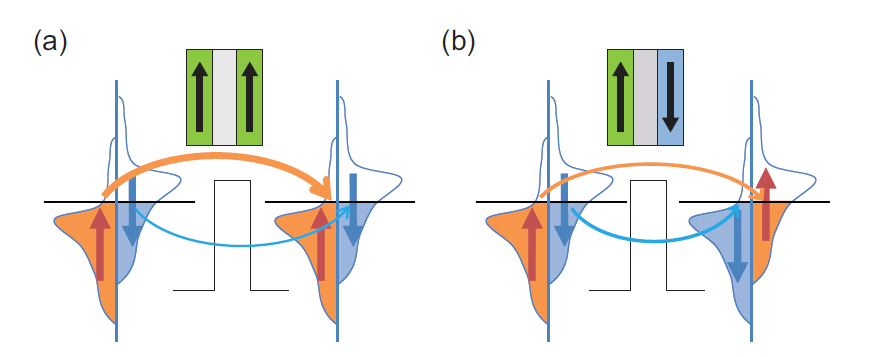
\includegraphics[width=1.0\textwidth]{fig/TMR.PNG}
\label{TMR}
\caption{Illustration of tunnel magnetoresistance effect. (a)Configuration of two layers are parallel.(b)Configurations of two layers are anti-parallel.}
\end{figure}


\begin{equation}
\label{eq:conductance}
\begin{aligned}
G_{p} &\propto  \rho_{L\uparrow}\rho_{R\uparrow}  + \rho_{L\downarrow}\rho_{R\downarrow}
\\
G_{Ap} &\propto  \rho_{L\uparrow}\rho_{R\downarrow}  + \rho_{L\downarrow}\rho_{R\uparrow}
\end{aligned}
\end{equation}


where $G_P$($G_{AP}$) is the parallel(anti-parallel) conductance, $\rho_{L\uparrow}$ and$\rho_{L\downarrow}$($\rho_{R\uparrow}$ and$\rho_{R\downarrow}$) are densities of states for up and down spins of the left(right) ferromagnet. By definition, the spin polarization P is 
\begin{equation}
P = \frac{\rho_{\uparrow} - \rho_{\downarrow}} {\rho_{\uparrow} + \rho_{\downarrow}}
\end{equation}

Therefore the tunnel magnetoresistance ratio can be calculated as

\begin{equation}
TMR = \frac{R_{AP} - R_{P}}{R_{P}}= \frac{G_{P} - G_{AP}}{G_{AP}} = \frac{2P_LP_R}{1-P_LP_R}
\end{equation}

In early studies of MTJs,a TMR ratio of a few 10's of percent was achieved with amorphous aluminum oxide(AlO)barries. Most recently, single crystalline magnesium oxide(MgO) barries were predicted to provide a much higher TMR ratio due to the wavefunction match between the ferromagnetic electrodes and the tunnel barrier. TMR ratios of around 200 percent were then demonstrated and led to intensive studies in MgO bases MTJs mainly because of the high TMR ratio founded in this family\cite{Mg0}.


\section{Spin transfer torque}

Spin transfer torque refers to the torque between electrons and local magnetization. As it is shown in \ref{fig:electron}, the direction of incident electron is randomly distributed in all directions. When electrons are entering a ferromagnetic layer, due to the fixed magnetization of this FM layer, electrons are parallel to the local magnetization will have high probability of transmission and on the other hand, the electrons having opposite direction will mostly be reflected. As a result, transmitted electrons will be aligned to the local magnetization and reflected. In this process, the angular momentum of incident electrons has been changed by local magnetization. On the other hand, the local magnetization also experience torque from incident electrons as well. This torque is called the spin transfer torque\cite{STT} \cite{Currenttorque} and can provide an efficient way to manipulate local magnetization as we shall see next.

\begin{figure}[ht]

  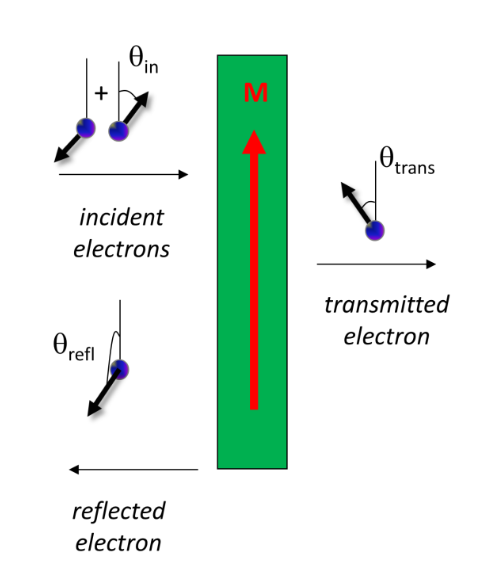
\includegraphics[width=60mm]{fig/electron.png}
  \centering
  \caption{Schematic of electrons transmitting through and getting reflected from ferromagnet metal, with the transverse spin component absorbed during the process.  }
  \label{fig:electron}
\end{figure}

Magnetic tunnel junction is the main device we have been studied. The device has a a structure of two ferromagnetic layers separated by a spacer. The mulitilayers are patterned into a elliptically-shaped nanopillar withe size normally around 60nm. The top and bottom of the devices are connected to electrical leads to allow current to pass perpendicularly through the multilayers.

The dynamics of the magnetization in the presence of spin transfer torque can be described by the classical Landau-Lifshitz-Gilbert(LLG) equation including an additional term for the spin torque:

\begin{equation}
\frac{dM}{dt} = \gamma M \times H_{eff} + \alpha M \times \frac{dM}{dt} + g(\theta)\frac{\gamma \hbar I}{eV_{free}M_s}M \times(M \times M_{fix})
\end{equation}

where $H_{eff}$ is the total effective field including the applied field $H_{applied}$ and the anisotropy field $H_{ani}$ and $\alpha$ is the damping constant. The first term is the field torque term which makes the magnetization precess around the effective field direction. The second term is the damping torque which relates the energy dissipation. On average it points towards the equilibrium position of the magnetization, so that without any external excitation the magnetization will relax back to the equilibrium. The third term is the spin transfer torque. The direction of this torque depends on the direction of the electron flow. For electron flow from the fixed layer to the free layer, this torque is in the same direction as the damping torque assuming the fixed layer also along the effective field direction, in this case spin transfer torque works as additional damping torque. On the other hand, for electron flow from the free layer to the fixed layer, this torque works against the damping torque and thus can reduce the relaxation.

The first case we discussed is of less interest. For the second case we have the competition between spin transfer torque and damping torque\cite{Bias}. Usually the spin transfer torque is small compared to the field torque. So the effect of spin transfer torque can be viewed as either increasing or decreasing the amplitude of the magnetic precession. In general, the magnetic dynamics excited by spin transfer torque can be categorized in to two types: switching and persistent precession.

\begin{figure}[h!]
\centering
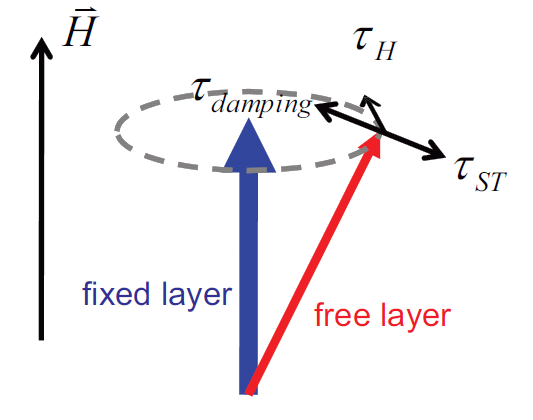
\includegraphics[width=0.5\textwidth]{fig/dampingtorque.PNG}
\label{Torque}
\caption{Direction of torques presented in the system.}

\end{figure}

\section{Magnetic Tunnel Junctions with Perpendicular Magnetic Anisotropy}

\subsection{Critical Switching Voltage}

In this section we would like to derive the critical switching voltage of the Magnetic Tunnel Junction(MTJ). We would like to prove that the critical voltage is symmetric between the Anti-Parallel state and the Parallel state, which is an important reason why it is crucial to characterize the MTJ in terms of bias voltage, not the bias current as used in many other magnetic materials system.

The critical switching current is given by\cite{SlonSwitching}
\begin{equation}
    I_{c0} = 2 \alpha \frac{\gamma e}{\mu_B \eta}E
\end{equation}
Here $\alpha$ is the Gilbert damping constant , $\gamma$ is gyromagnetic ratio, e is the elementary charge  $\eta$ is the spin-transfer efficiency. The energy barrier $E$ is given by
\begin{equation}
    E = M_s H_K V / 2
\end{equation}
Here $M_s$ is the saturation magnetization, $H_K$ the anisotropy field, V is the volume. We can further rewrite the spin transfer efficiency as
\begin{equation}
    \eta = \frac{P}{2}\frac{1}{1+P^2 \cos{\theta}}
\end{equation}

P is the polarization factor given by
\begin{equation}
    P = \sqrt{\frac{G_P - G_{AP}}{ G_P + G_{AP}} }       
\end{equation}
The conductance of the Magnetic Tunnel Junction can be given by\cite{MTJConductance}
\begin{equation}
    G(\theta) = \frac{1}{2} (G_P + G_{AP}) + \frac{1}{2} (G_P - G_{AP}) \cos{\theta}
    = \frac{G_P + G_{AP}}{2}\big[ 1+P^2\cos{\theta} \big]
\end{equation}
If we define $G_0 = \frac{G_P + G_{AP}}{2}$ as the average conductance and use the Ohm's Law, the critical switching voltage for MTJ should be
\begin{equation}
    V_{C0} = \frac{I_{C0}}{G(\theta)} = 2\alpha\frac{\gamma e}{\mu_B}E\frac{1}{\eta G(\theta)}
\end{equation}
Replacing gyromagnetic ratio with g factor $\gamma = \frac{g \mu_B}{\hbar}$, the above equation becomes
\begin{equation}
    \label{eq:criticalV}
    V_{C0} = 4\alpha\frac{ge}{\hbar P G_0}E
\end{equation}

One can easily find from Eq.\ref{eq:criticalV}, it is clear that the critical switching voltage of MTJs do noes depend on the relative configurations of two ferromagnetic layers of the MTJ. Parral and Anti-Parallel states have the same critical voltage(in this macrospin model).  




\section{Magnetic Switching}

At zero or small field, both direction along the easy axis correspond to local energy minimums so it is possible to switch the magnetization between these two directions with spin transfer torque. For example, for a device with both free and fixed layers keeping at the easy axis direction and parallel to each other, if we flow a positive current defined as current flow from free to fixed layer, according to previous analysis, the spin transfer torque acts on the free layer is pointing away from the fixed layer and destabilizes this configuration so that the magnetic moment of the free layer goes into a precession around the easy axis. If we keep increasing the current, the amplitude of the free layer precession increases until it reaches the energy barrier which is around 90 degree. After the free layer changes direction, now the spin transfer torque will act as damping torque again and stabilize the magnetization. Similarly, if the magnetic tunnel junction starts in the anti-parallel configuration, a strong enough negative current can switch the free layer back to the parallel configuration. If we monitor the resistance of the device, it will exhibit a hysteresis loop as we sweep the current, as shown in the example

\begin{figure}[h!]
\centering
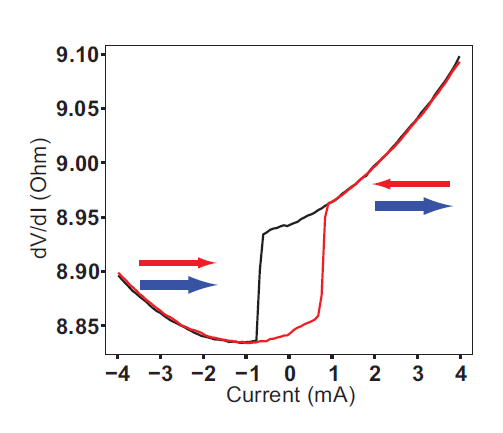
\includegraphics[width=0.5\textwidth]{fig/DC.PNG}
\label{DC}
\caption{Differential resistance with respect to dc current. Arrows indicate magnetic state to be either parallel and anti-parallel.}

\end{figure}

The critical switching current $I_c$ is defined as the current required to achieve switching at zero temperature(no thermal excitations)  . Above $I_c$, the spin torque is stronger than the damping torque and drives the free layer moment to switch direction.[Fig] illustrate the switching process. The switching proceeds via a precessional motion of the magnetization with increasing amplitude\cite{subswitch}. The switching time is defined as the following :


\begin{figure}[!ht]
\centering
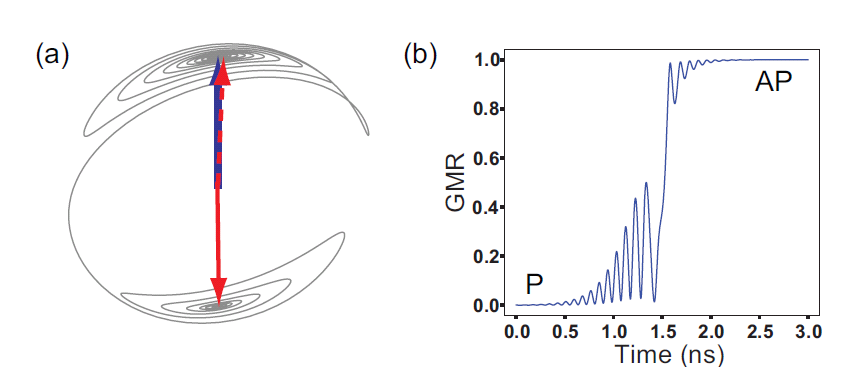
\includegraphics[width=1.0\textwidth]{fig/switching.PNG}
\label{Switching}
\caption{An example of a simulated spin transfer switching event.(a)Switching trajectory. Dotted lines show initial state of free layer. Solid line shows the switching (b) Normalized resistance value as a function of time}
\end{figure}

\begin{equation}
t_s \propto \frac{1}{I-I_c}
\end{equation}

Now if the applied current is smaller than the critical current, the spin torque is not strong enough to drive the free layer moment to directly overcome the energy barrier to achieve switching but only to excite magnetic precession at small amplitudes. At finite temperatures, switching can still occur due to thermal excitations. This thermal-assisted magnetization reversal can be described by the Neel-Brown relaxation time:
\begin{equation}
P(t) = 1 - exp(-t/\tau)
\end{equation}
where t is the observation time, and $\tau$ is the relaxation time which is given by
\begin{equation}
\tau = \frac{1}{f_0}\exp{E_b/k_B T}
\end{equation}
Here $f_0$ is the attempt frequency, $E_b$ is the energy barrier and T is the temperature. Thermal assisted switching can be modeled by a fluctuating field with a Gaussian stochastic process. The relaxation time $\tau$ can be modified as the following:

\begin{equation}
\tau = \frac{1}{f_0}\exp [\frac{E_b}{k_B T}(1 - \frac{I}{I_c})]
\end{equation}


\section{Ferromagnetic Resonance}
We start with the cordinate system that the place $y=0$ is subjected to a d.c. field $H_z$ and a weak microwave field $H_x$. The magnetization $\boldsymbol{M}$ and the angular momentum density $\boldsymbol{J}$ are related by $\boldsymbol{M} = \gamma \boldsymbol{J}$\cite{Kittel1947}\cite{Kittel}, where $\gamma$ is the gyromagnetic ratio. The equation of motion $\frac{\partial J}{\partial t} = \big[\boldsymbol{M} \times \boldsymbol{H}]$ can be written as 
\begin{equation}
    \label{eq:Mmotion}
    \frac{\partial \boldsymbol{M}}{\partial t} = \gamma \big[\boldsymbol{M} \times \boldsymbol{H}]
\end{equation}
If we want to solve for the general resonance condition for a ellipsoid with major axis parallel to the x, y, z axes of the coordinate system, we first have the demagnetization factor: $N_x$,$N_y$ and $N_z$. The effective values of the magnetic field components are
\begin{equation}
\label{eq:MvsT}
\begin{aligned}
{H_x}^i &= H_x - N_x M_x \\
{H_y}^i &=  - N_y M_y \\
{H_z}^i &= H_z - N_z M_z \\
\end{aligned}
\end{equation}

The values ${H_x}^i$  ${H_y}^i$ and ${H_z}^i$ should be used when substituting $H$ in Eq.\ref{eq:Mmotion}. Now we can decompose Eq.\ref{eq:Mmotion} into 

\begin{equation}
\label{eq:MvsT}
\begin{aligned}
\partial M_x \char`\/ \partial t &= \gamma\big[H_z + (N_y - N_z) M_z] M_y   \\
\partial M_y \char`\/ \partial t &= \gamma\big[M_z H_x - (N_x - Nz)M_x M_z - MxHz]   \\
\partial M_z \char`\/ \partial t &\approx 0
\end{aligned}
\end{equation}

If we solve these equations with time dependent $\exp{i \omega t}$, the susceptibility $\chi_x = M_x / H_x$ is given by 

\begin{equation}
    \label{eq:suscept}
    \chi_x = \frac{\chi_0}{1 - (\omega / \omega_0)^2}
\end{equation}

where
\begin{equation}
    \label{eq:chi0}
    \chi_0 = \frac{M_z}{H_z + (N_x - Nz)Mz}
\end{equation}
and the resonance frequency is given by 
\begin{equation}
    \label{eq:resonance}
    \omega_0 = \gamma \big\{ \big[Hz+(N_y - N_z)M_z] \times \big[Hz+(N_x - N_z)M_z]          \big\}^\frac{1}{2}
\end{equation}

From Eq.\ref{eq:resonance} we can have some special cases:
\begin{enumerate}
  \item Plane ($N_x = N_z = 0$;$N_y = 4 \pi$)
  \begin{equation}
      \omega_0 = \gamma (B_z H_z)^\frac{1}{2}
  \end{equation}
  \item Sphere ($N_x = N_y = N_z = 4\pi/3$)
  \begin{equation}
      \omega_0 = \gamma H_z
  \end{equation}
  \item Infinite Circular Cylinder ($N_x = N_y = 2\pi$;$N_z = 0 $)
  \begin{equation}
      \omega_0 = \gamma (H_z+2\pi Mz)
  \end{equation}
\end{enumerate}
It is often that the ferromagnetic crystals energies depends on the relative magnetization orientations and in order to minimize the total energy, the magnetizations would align with the easy axis. This is called the anisotropy energy. If the anisotropy is uniaxial, the first-order magnetic anisotropy can be written as 
\begin{equation}
    f = K_1 {\sin{\theta}}^2
\end{equation}
where f refers to unit volume of material. $\theta$ is the angle between the magnetizations and the easy axis of the crystal. $K_1$ is the first-order anisotropy constant. To account for the effect on resonance conditions, it is easier to consider the effect in terms of an equivalent magnetic field. The equivalent field $H^e$ is defined as
\begin{equation}
    \partial f \char`\/ \partial \theta = M_s \times H^e
\end{equation}
It should be noted that the direction of effective field $H^e$ is still arbitrary and without lose any generality, we can express the effective field in terms of effective demagnetizing factor $N^e$ as
\begin{equation}
    \begin{aligned}
        {H_x}^e &= - {N_x}^e M_x \\
        {H_y}^e &= - {N_y}^e M_y \\
    \end{aligned}
\end{equation}
The resonance condition from Eq.\ref{eq:resonance} can now be modified as 
\begin{equation}
    \label{eq:resonanceKu}
    \omega_0 = \gamma \big\{ \big[Hz+(N_y + {N_y}^e - N_z)M_z] \times \big[Hz+(N_x + {N_x}^e - N_z)M_z]          \big\}^\frac{1}{2}
\end{equation}
I
\section{Spin-torque Ferromagnetic Resonance}

As we mentioned above, when the spin transfer torque is small, the magnetization will not reverse however experience a persistent precession. By applying AC current, excited magnetic precession can be detected by measuring a mixing DC voltage from the product of the resistance oscillation and the ac current. This Spin-transfer Ferromagnetic Resonance (ST-FMR) \cite{Sankey2006}\cite{Tulapurkar2005} is similar to the traditional ferromagnetic resonance, but can be performed in much smaller devices. The ST-FMR technique can be used to characterize important material properties such as voltage-controlled-anisotropy\cite{VCMA1}\cite{Jian}\cite{Wang2012}, magnetic damping\cite{PRLdamping}, field-like torque\cite{Sankey2008} along with the spectrum of magnetic excitations of the MTJ\cite{excitation1}\cite{excitation2}, which is not important for understanding basis physic phenomena like spin-tunnel process but also essential for characterizing and optimizing the MTJs for future applications. In Chapter 3, I will describe an improved technique to measure Spin-torque Ferromagnetic Resonance with field modulations.









%\chapter{Field-Modulated Spin-torque Ferromagnetic Resonance}

\section{Spin-torque Ferromagnetic Resonance}

Ferromagnetic resonance (FMR) is the main technique to study dynamical properties
of magnetic materials. However, “conventional FMR detection methods lack the sensitivity
to measure individual sub-100-nm-scale devices that are of interest for fundamental
physics studies and for a broad range of memory and signal-processing applications”\cite{Sankey2006}.

Sankey and Tulapurkar et al. demonstrated that they can excite precession not by applying
an ac magnetic field as is done in other forms of FMR, but by using the ac spin-transfer
torque from a spin-polarized ac current.When an alternating current is applied to the
sample\cite{Sankey2006}\cite{Tulapurkar2005}, spin transfer torque induces magnetization dynamics, leading to a changing sample resistance from the sample magnetoresistance. Alternating current and resistance get mixed and give rise to a direct voltage, which can be measured using lock-in technique. By
sweeping the frequency of the applied alternating current, a peak in the direct voltage
generated by the sample can be observed when the applied frequency matches the
resonance frequency of the sample. This technique is called spin-torque ferromagnetic
resonance\cite{Sankey2006} and has been widely used to understand magnetization dynamics induced by
spin transfer torque. Analysis of the resonance frequencies, amplitudes, linewidths, and
line shapes as a function of microwave power, dc current, and magnetic field provide
detailed new information about the exchange, damping\cite{FMR_damping}\cite{FMR_damping2}, and spin transfer torques that
govern the dynamics in magnetic nanostructures\cite{Sankey2006}.

When the spin polarized current is applied near the resonance frequency, it can drive the precession of magnetization by effectively pushing and pulling the
magnetization (depending on the instantaneous polarity of the RF current) in phase with its
natural precession. In the case of MTJs, the fixed layer acts as a spin filter which polarizes the current passing through the free layer in the direction of the fixed layer’s magnetization. In this discussion, it is assumed that the fixed layer magnetization is ideal and completely locked in place. This oscillation of the free layer magnetization will also produce an oscillation of the device resistance due to the varying relative angle between fixed and free layer
magnetizations. The time-dependent
resistance can be expressed as the expansion \cite{Sankey2006}:
\begin{equation}\label{eq:RvsT}
R(t) = R_{0} + \Delta R(t) = R_{0} + Re(\sum_n \Delta R_{nf} e^{in\pi ft}) 
\end{equation}

When the $\Delta R_{nf}$ can be can be complex. Since the fixed layer is supposed to be stationary, the resistance thus oscillates as the magnetization of the free layer m,which is the solution of the LLGS equation. The mixing voltage signal being measured can be composed of rather complex form, however, it is possible to write the voltage as
\begin{equation}\label{eq:FMR}
V_{mix} = V_{s}S(\omega) + V_{a}A(\omega)
\end{equation}
Where $\omega$ is the driven frequency and $V_{s}$ and $V_{a}$ are functions of the spin-torque vector and other magnetic parameters. In this case, the fitting can be simplified as only four fitting parameters. In order to study magnetic information such as anisotropy field and Gilbert damping parameter, one can measure the spectrum and fit fro resonance frequency and linewidth as a function of applied field. The theoretical model used here is given by the Kittel equation\cite{Kittel}.
\begin{equation}\label{eq:Kittel}
f_{res} = \gamma(H_{k} \pm |H_{dip}| + H_{ext})
\end{equation}
Here $f_{res}$ is the resonance frequency extracted from fitting the curve. $H_{dip}$ is the center of hysteresis loop and $H_{ext}$ is the external magnetic field. The Gilbert damping parameter, given the easy axis approximation, is 
\begin{equation}\label{eq:damping}
\alpha = \frac{\Delta f_{res}}{f_{res}}
\end{equation}
It should be noticed that in this Equation \ref{eq:damping}, the linewidth $\Delta f_{res}$ is the half-width-at-half-maximum(HWHM).


\section{Experimental Technique}

However, this frequency-domain ST-FMR method suffers from frequency-dependent non-magnetic background signals due to non-linearities and impedance mismatches within the microwave circuit. For example, measurements of MTJ with collinear free and pinned layer magnetizations (the STT-MRAM geometry) are challenging with this conventional ST-FMR technique because magnetic signals are typically weaker than the frequency-dependent non-magnetic background signal. Indeed, in the ideal case, device structures with a single perpendicular uniaxial anisotropy axis and preserved rotational symmetry around the axis should create no spin transfer torque and thus would not resonant at FMR frequencies\cite{chris}. On the other hand, measuring ST-FMR at collinear geometry is important. When the magnetizations of free layers are not parallel to, but instead lags behind the external field direction, the linewidth from FMR spectra would be broadened by this magnetic dragging effect\cite{dragging}. Applying external magnetic field in the easy-axis direction would be convenient for quantitative spin wave mode analysis.  For example, measurements of MTJ with collinear free and pinned layer magnetizations (the STT-MRAM geometry) are challenging with the rectification ST-FMR because magnetic signals are typically weak. Fig.\ref{fig:Amp} shows a typical spectrum measured by conventional ST-FMR with amplitude modulations. Despite the excitations of several spin wave modes, the spectrum has changing background and lots of standing wave from the circuit, thus it would be very hard to quantitatively fit to extract resonance frequency and linewidth.



\begin{figure}[h!]
\centering
    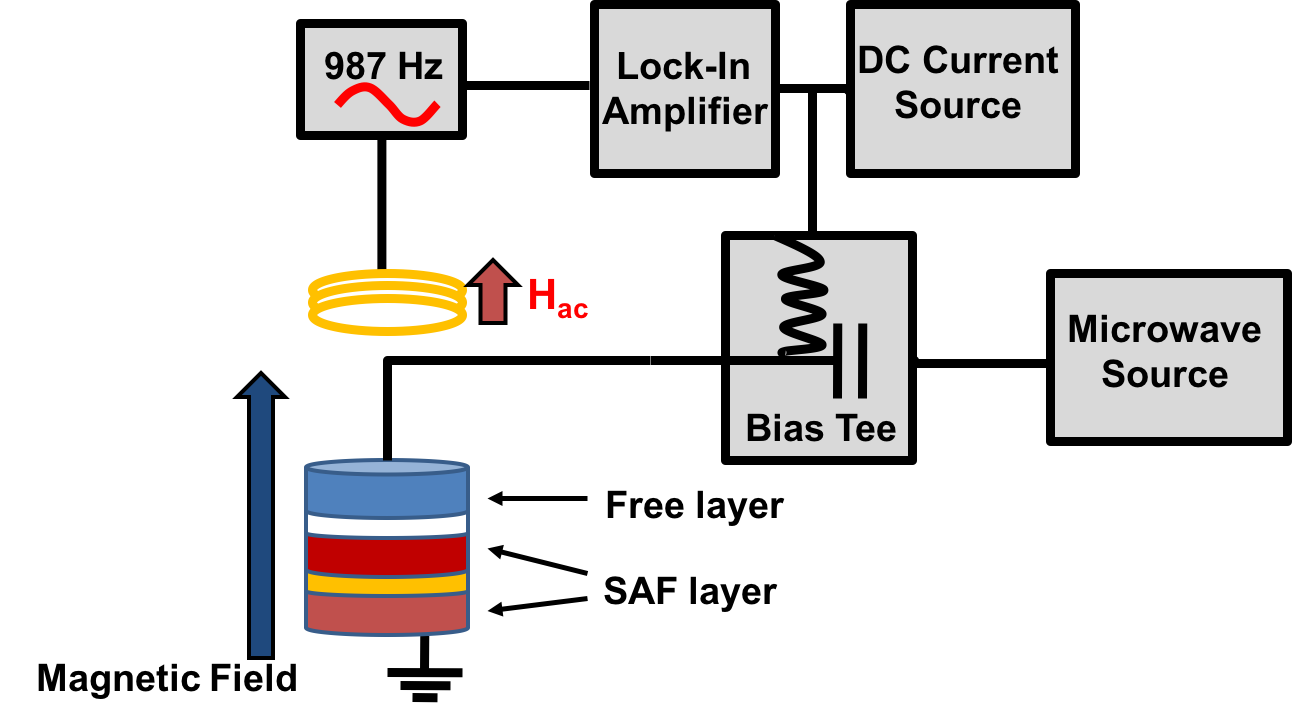
\includegraphics[width=0.8\textwidth]{fig/FieldMod/set_up.png}
    \caption{Sketch of our field-modulation set-up.}
    \label{fig:FMR_set_up}
\end{figure}





\begin{figure}[!ht]
\centering
\subfigure{\label{fig:Amp}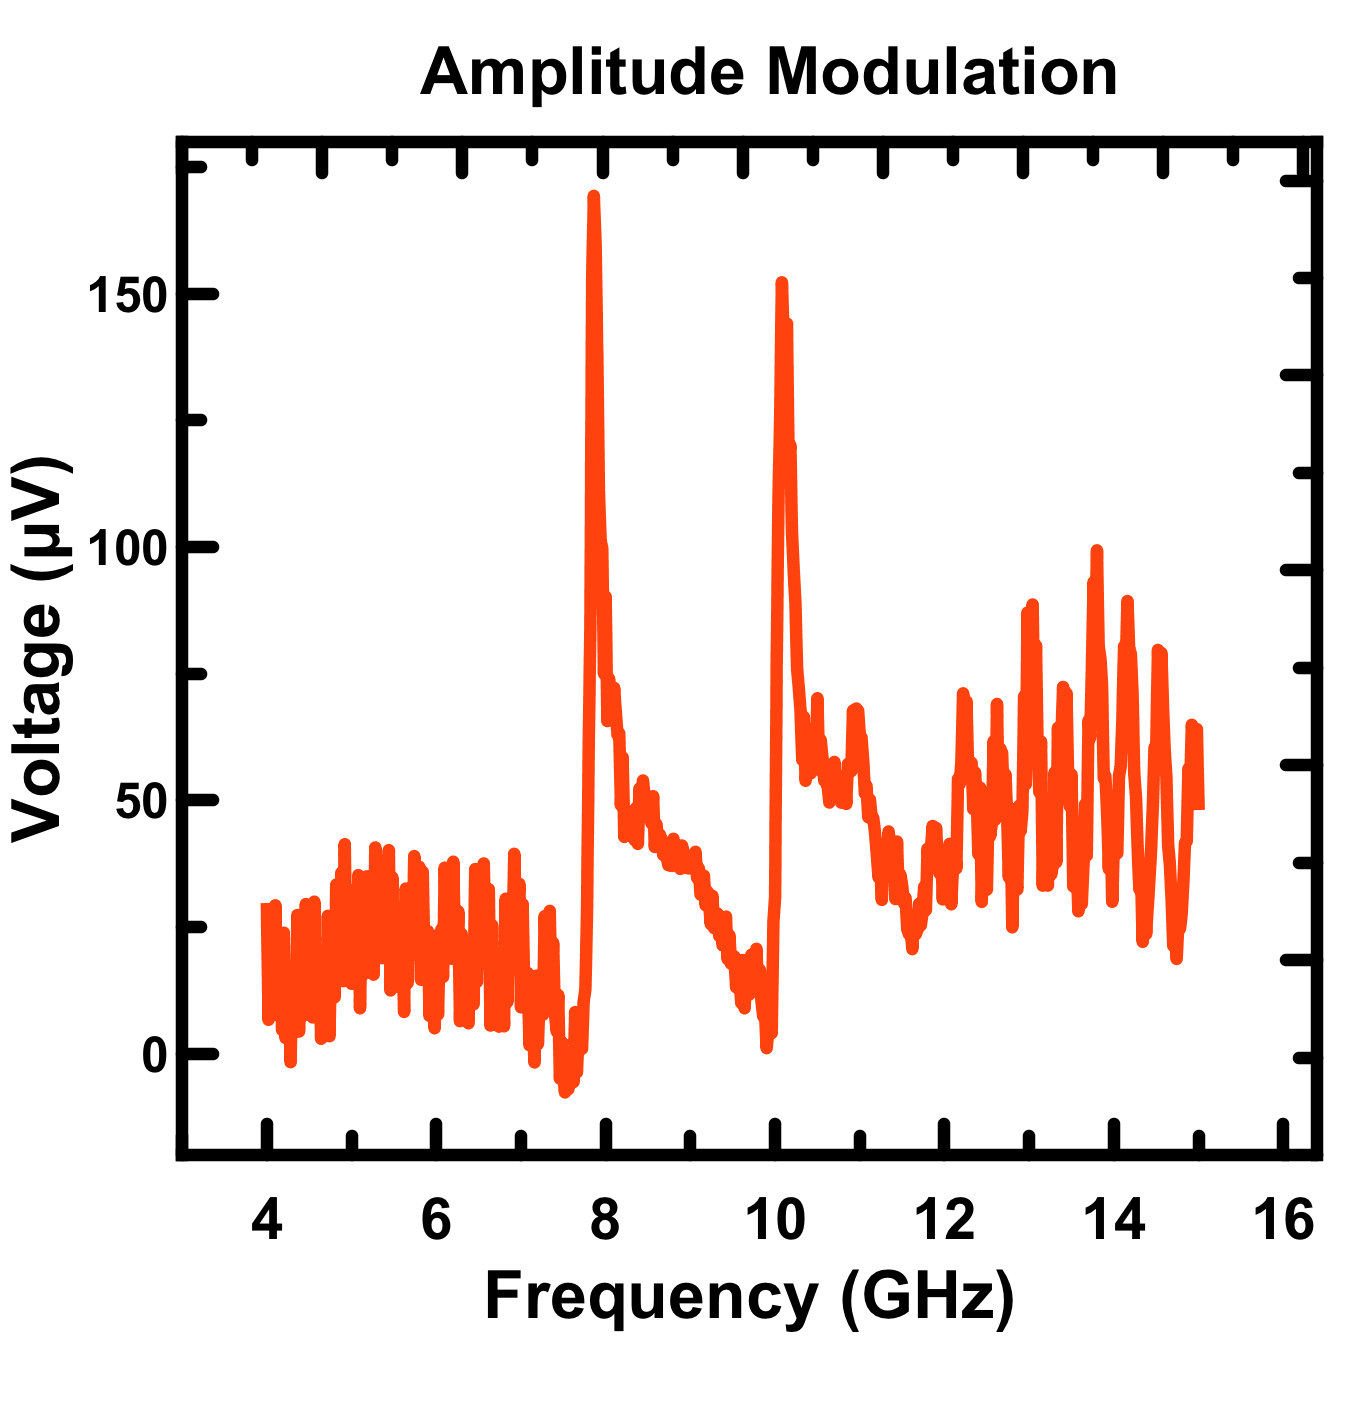
\includegraphics[width=70mm]{fig/FieldMod/AmpMod.png}}
\subfigure{\label{fig:Field}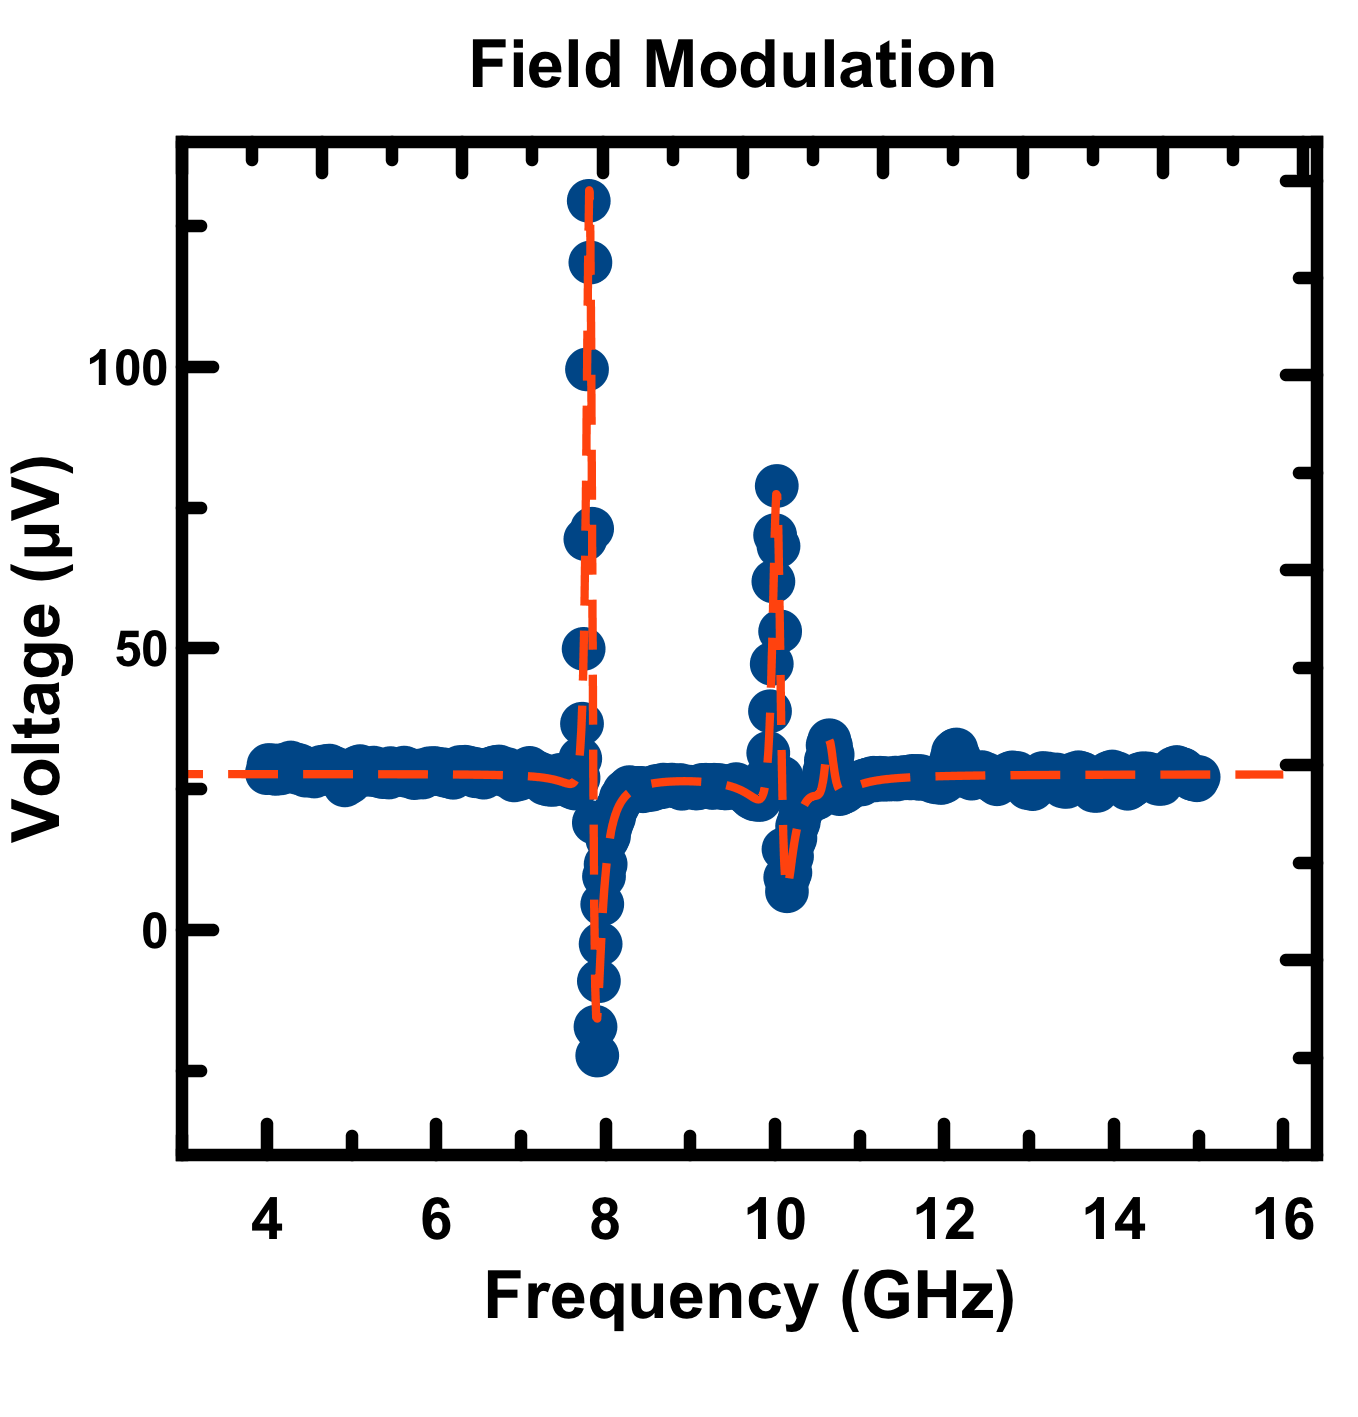
\includegraphics[width=70mm]{fig/FieldMod/FieldMod.png}}
\caption{(a) Typical ST-FMR spectrum taken with conventional amplitude modulation.(b) ST-FMR spectrum taken with field modulation at the same sample.}
\end{figure}





To solve this problem, We make ST-FMR measurement with field modulation technique\cite{FieldMod}. A modulation coil is placed just above the sample as shown in Fig.\ref{fig:FMR_set_up}. We then apply kHz-range sinusodal current of a few Amperes in the coil and generate a few Oersteds alternating magnetic field. The modulation field from the coil is perpendicular to the nanopillar. A continuous microwave current is applied to the sample via a bias tee, and a rectified voltage generated by the sample is measured by a lock-in amplifier at the field modulation frequency. In this case, by sweeping the driving frequency, any non-magnetic background noise would be eliminated. Fig.\ref{fig:Field} shows a typical field-modulation spectrum taken at the same sample comparing with Fig.\ref{fig:Amp}(a). Now we have a much better flat baseline and the standing wave is greatly reduced from the signal.


\begin{figure}[!ht]
\centering
\subfigure{\label{fig:MR}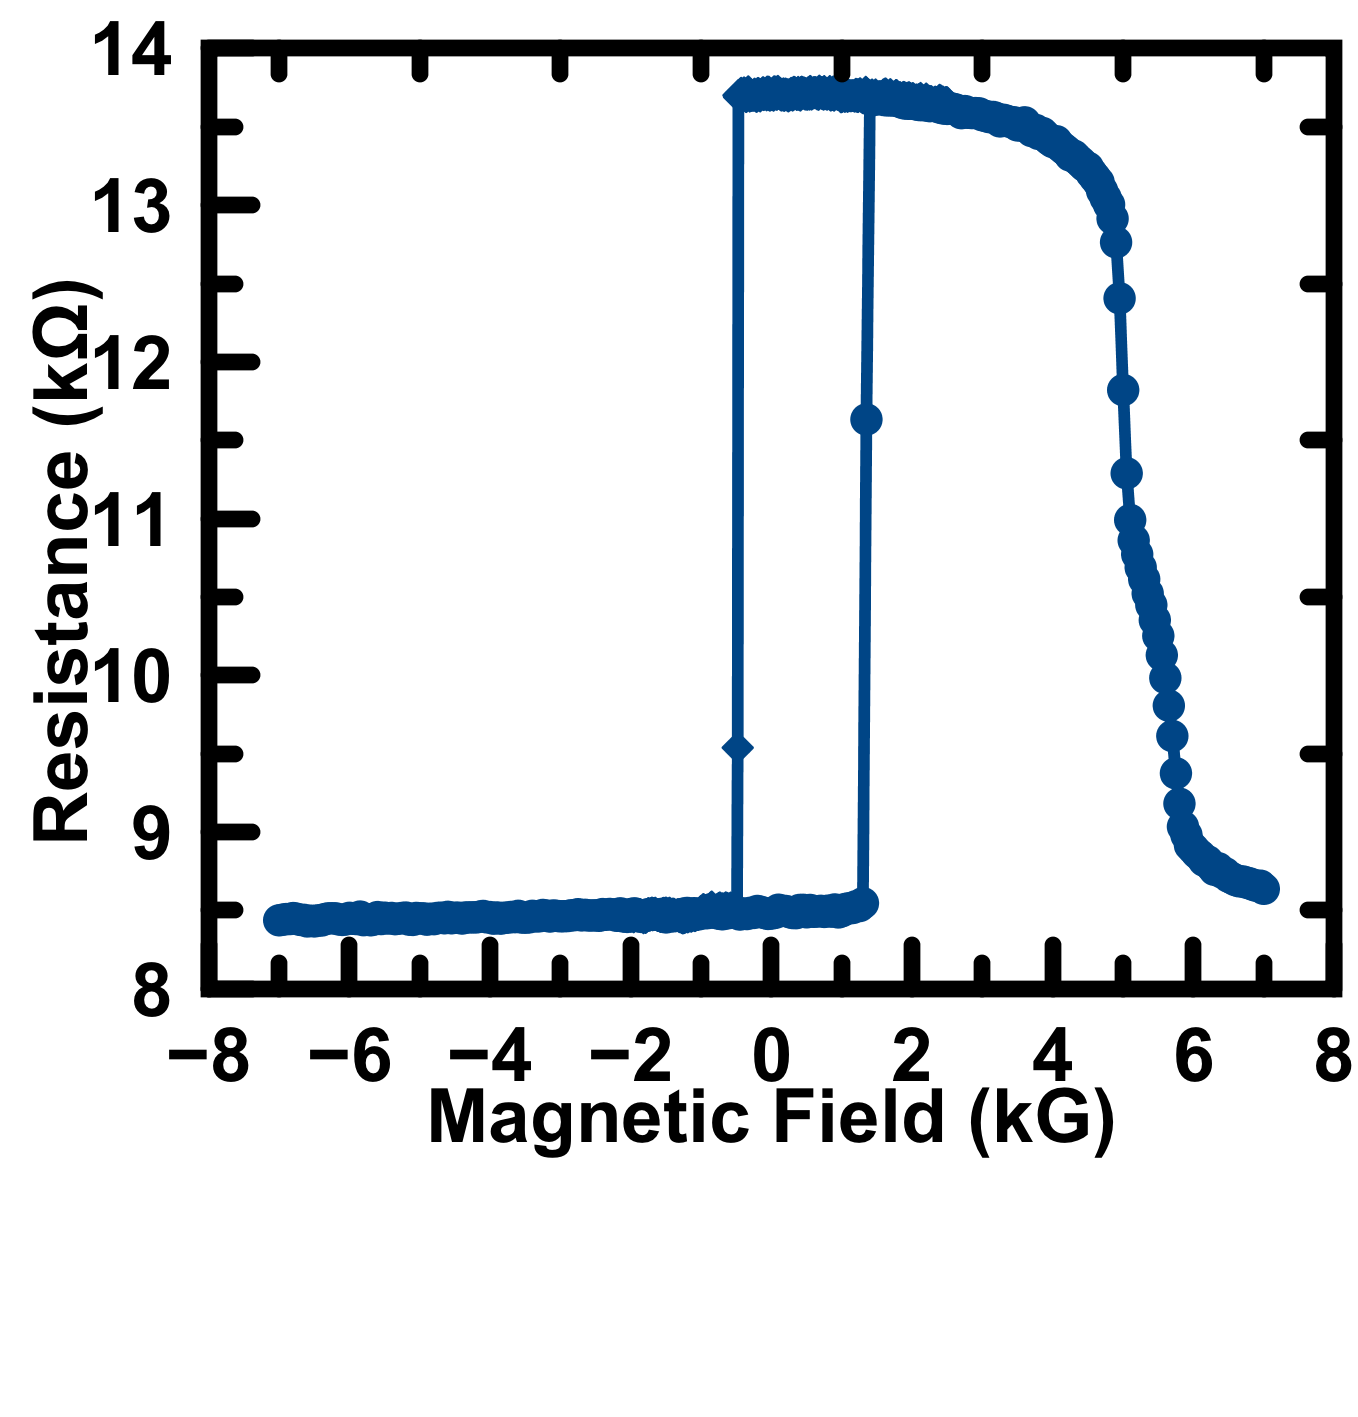
\includegraphics[width=70mm]{fig/FieldMod/MR.png}}
\subfigure{\label{fig:Spectrum}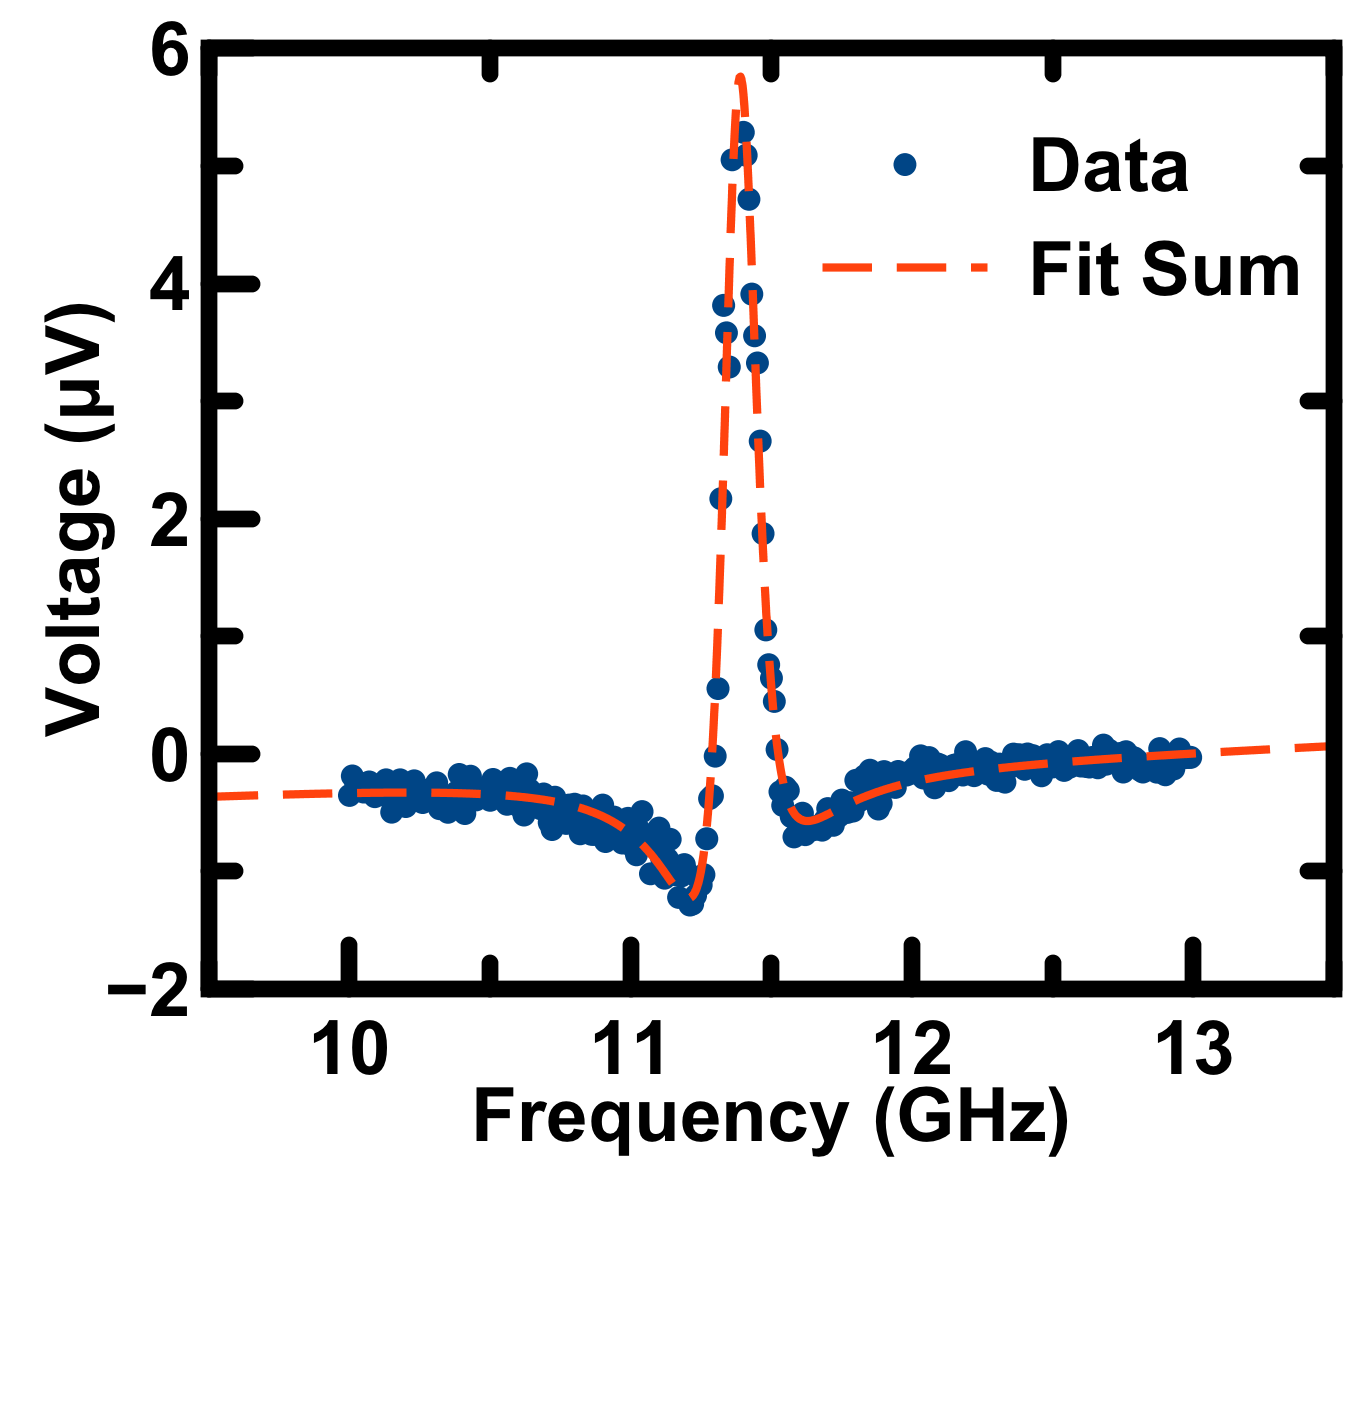
\includegraphics[width=70mm]{fig/FieldMod/Spectrum.png}}

\caption{(a)Magneto-resistance plot of the sample studied. SAFTop layer start to flop around 4.5kG. (b)Blue dot:Typical ST-FMR spectrum with only lowest-frequency mode. Red dash line: Fitted curve to extract resonance frequency and linewidth.}
\end{figure}

The MTJ nanopillar we have measured has a lateral size of 65*30nm with a stadium shape: approximately half-circular on both ends of a rectangular. The main functional layers structure of our sample are SAFBottom(1.67)/SAF spacer(0.41)/SAFTop(1.1)MgO(0.8)FreeLayer(2.4) multilayer(thickness in nm). Fig.\ref{fig:MR} shows the magneto-resistance plot with magnetic field applied perpendicular to the sample. Around 4.5kG, the resistance of the MTJ start to decrease and eventually switch back to low-resistance parallel state. This is due to the flopping of SAFTop layer\cite{Spinflop}. We identify 4.5kG to be the breakdown field and will use it for later discussion.Fig.\ref{fig:Spectrum} shows the ST-FMR spectrum focusing on the lowest-frequency mode. We are now going to derive the mathematical equation to extract resonance frequency and linewidth from the curve.



\section{Gilbert Damping Evaluation}

As we discussed in the previous chapter, the line shape $V_{mix}(f)$  without field modulation is a sum of symmetric $S(f)$ and antisymmetric $A(f)$ Lorentzians $V_{mix}(f) = V_{s}S(f) + V_{a}A(f)$, where $S(f) = \frac{1}{1+(f-f_{r})^{2}/ \sigma_{r}^{2}}$, $A(f) = \frac{(f-f_{r})/\sigma_{r}}{1+(f-f_{r})^{2}/ \sigma_{r}^{2}}$, $f_{r}$ is the resonance frequency and $\sigma_{r}$ is the linewidth. When the modulation field is small, the RMS voltage signal  $\tilde{V}_{mix}(f)$ measured by the lock-in amplifier is proportional to the first derivative of the rectified voltage  $V_{mix}(f)$ with respect to the modulated variable-the external magnetic field $B$.


\begin{equation}
\begin{aligned}
  \tilde{V}_{mix}(f) = & B_{m}\frac{dV_{mix}(f)}{dB} = B_{m}[\frac{dV_{s}}{dB}S(f) + \frac{dV_{s}}{dB}A(f) \\ 
  & + \frac{1}{\sigma_{r}}\frac{d\sigma_r}{dB} 
  \times (2 V_{s} A^{2}(f) + V_{a}[2A^{3}(f)/S(f) - A(f)]) \\
 & + \frac{1}{\sigma_r}\frac{df_{r}}{dB}(2V_{s}S(f)A(f) + V_{a}[A^{2}(f) - S^{2}(f)])]  
\end{aligned}
\end{equation}

Here $B_{m}$ is the RMS amplitude of the modulation field, and the last term proportional to $df_{r}/dB$ is usually dominant. If $V_{s}$ and $V_{a}$ are weak functions of magnetic field then the symmetric part of $\tilde{V}_{mix}(f)$ is proportional to $V_{a}$ and the anti symmetric part is proportional to $V_{f}$.


\begin{figure}[!ht]
\centering
\subfigure{\label{fig:Free}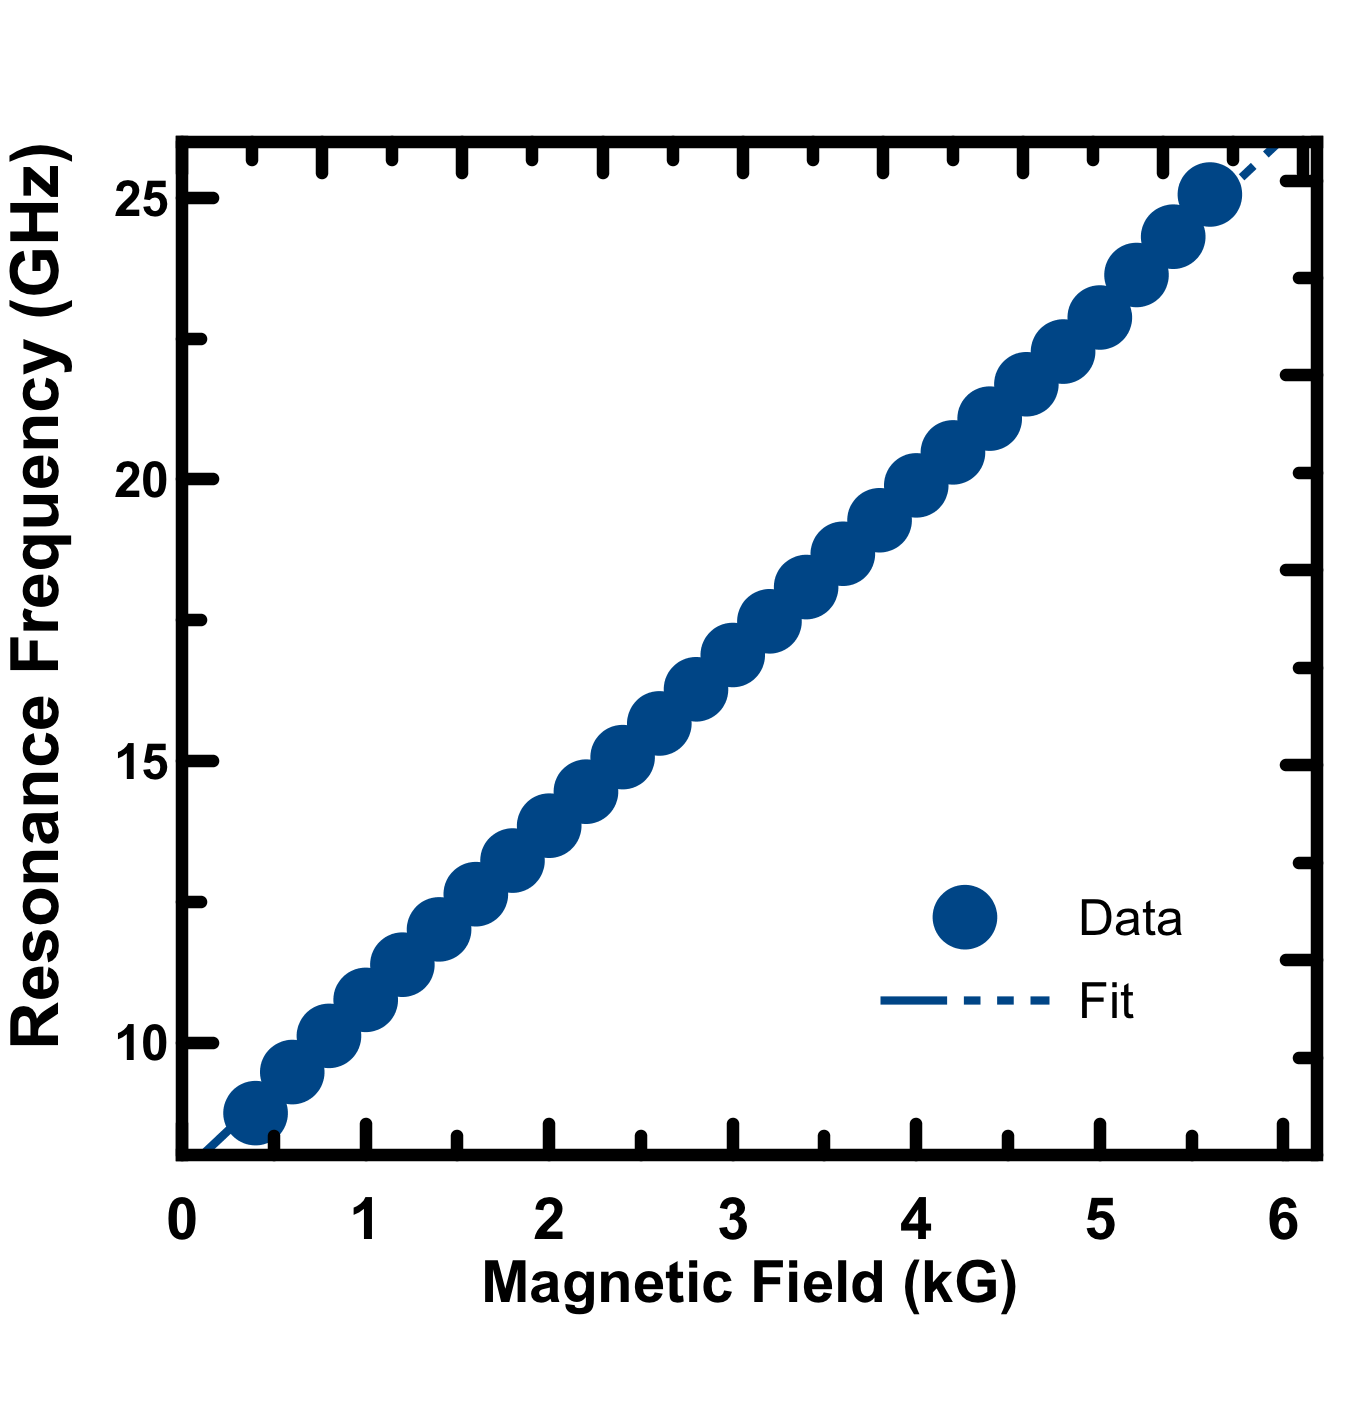
\includegraphics[width=75mm]{fig/FieldMod/Res_Field.png}}
\subfigure{\label{fig:LW}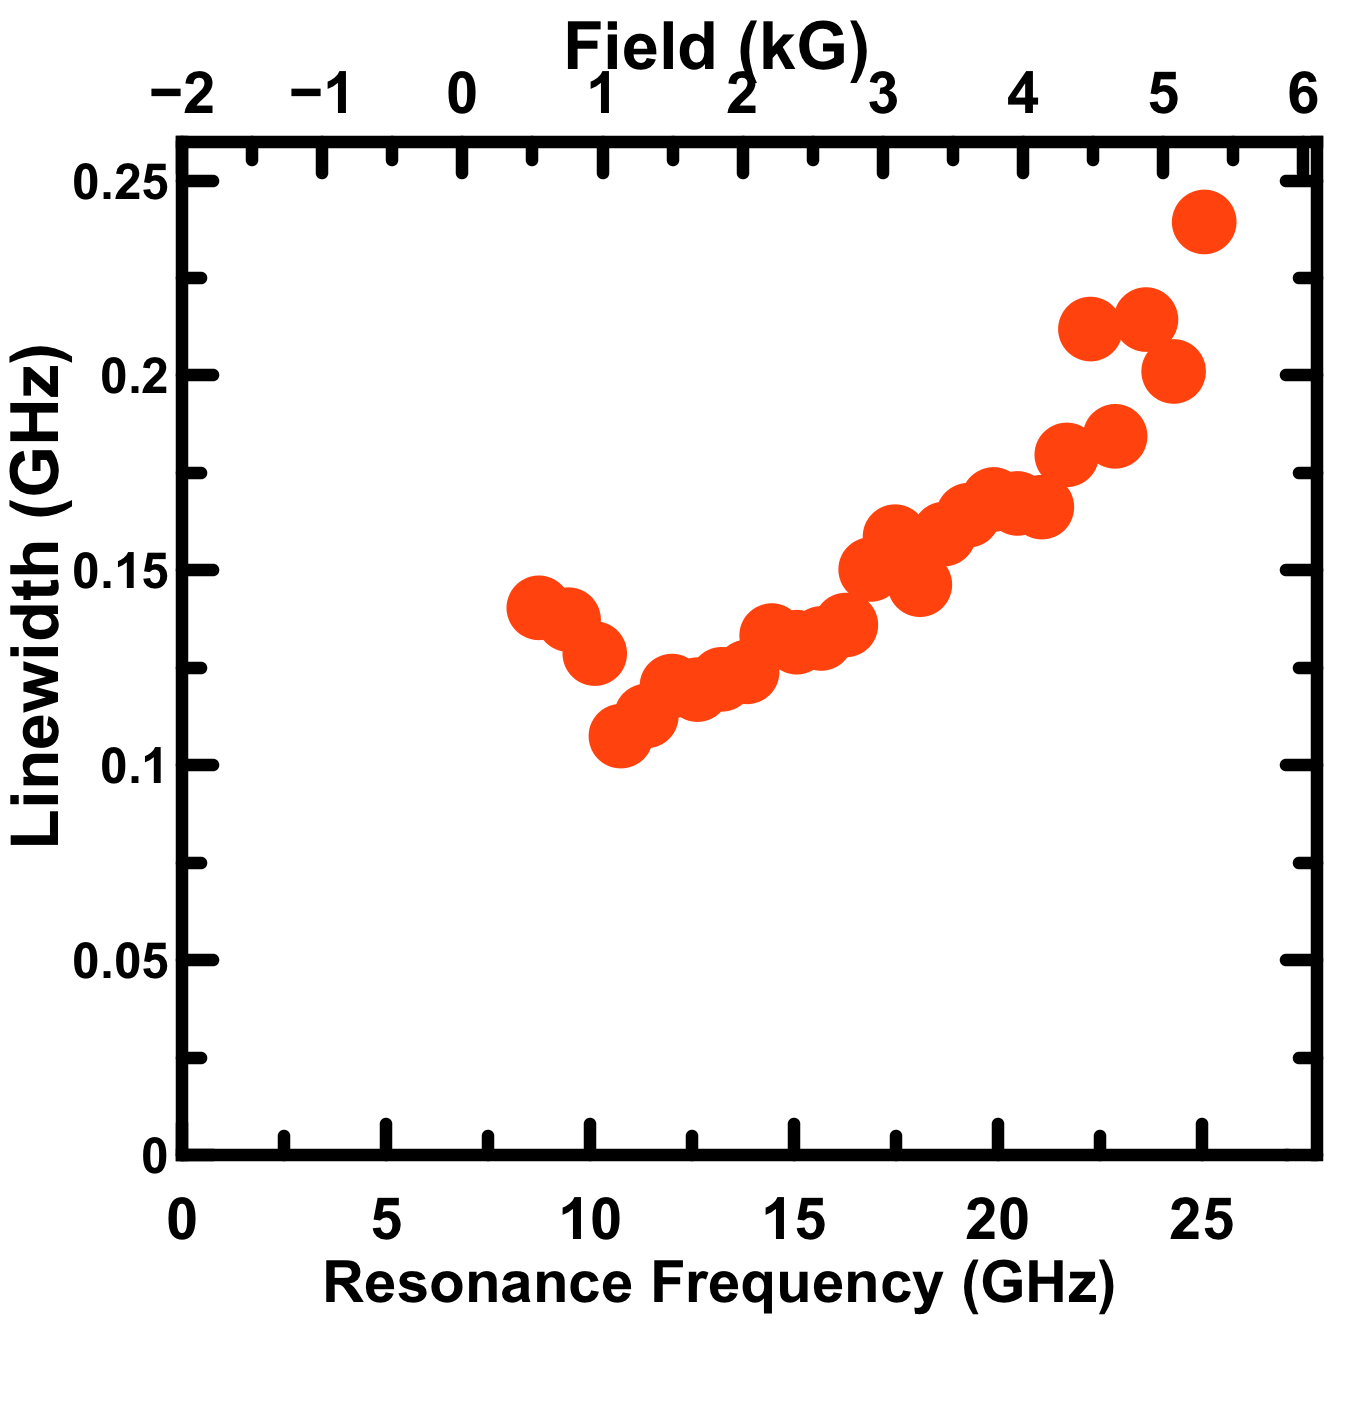
\includegraphics[width=75mm]{fig/FieldMod/Original_LW.png}}
\caption{(a) Fitted resonance frequency plotted against external magnetic field (b)Fitted linewidth plotted as a function of resonance frequency.}
\end{figure}

Fig.\ref{fig:Free} shows the fitted resonance frequency of the quasi-uniform modes respect to the external magnetic field. As we expect from Kittel equation, there is a good linear relation. Making an easy axis approximation, the Kittle equation is 
\begin{equation}
f = \gamma(H_{k} \pm |H_{dip}| + H_{ext})
\end{equation}
Here $H_{dip}$ is the center of hysteresis loop and $H_{ext}$ is the external magnetic field. The quasi-uniform mode frequency at zero field gives magnetic anisotropy field of the free layer ($H_{k}$ = 2.5 kG). 

Next we try to fit for the damping parameter. Precision measurements of the spectral linewidth of the quasi-uniform mode required some improvements of our ST-FMR setup. We found that standing waves in the microwave measurement circuit can introduce significant errors into the measured line width. In order to alleviate the standing wave problem, we introduced a significant length (1.5 – 2 meters) of a microwave cable between the sample and the bias tee used in the ST-FMR setup. This additional length acted as a microwave attenuator that does not generate significant signal reflection (adiabatic absorptive attenuator). Fig\ref{fig:cable} illustrates the degree of improvement of the ST-FMR signal quality offered by the cable attenuator – the spectral peak splitting artifact is completely eliminated and reliable measurements of the spectral linewidth become possible.

\begin{figure}[!ht]
  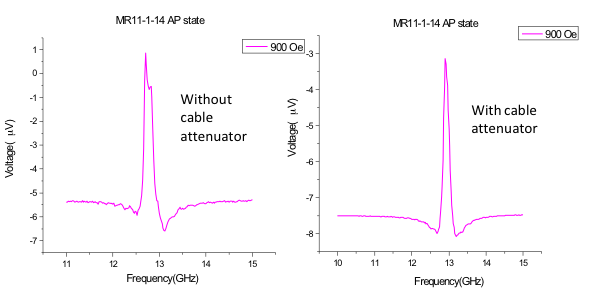
\includegraphics[width=0.8\textwidth]{fig/FieldMod/Improve-measure.png}
  \centering
  \caption{ST-FMR spectrum measured without a long attenuating cable attached to the sample (left) is significantly distorted by standing waves in the microwave circuit. (right) The same spectrum measured with a long attenuating cable eliminates the standing wave artifacts. }
  \label{fig:cable}
\end{figure}






Previous work has been shown that Gilbert damping parameter can be determined from the linewidth from the FMR signal\cite{Bias}. Fig.\ref{fig:LW} shows the linewidth plotted as a function of resonance frequency. We would expect to observe a linear relation if only considering Gilbert damping contribution. From our data,however,we can observe obvious two regions which deviate from a simple linear fitting. Firstly, at low frequency around 10GHz, the linewidth was clearly broadened and was larger than other region. Secondly, at higher frequency above 20GHz, the linewidth has more noise in terms of relative fluctuations. Moreover, if we try to fit the linewidth data and extrapolate to zero frequency, we found there is a large non-zero intercept. It is not clear whether this non-zero intercept is due to some inhomogeneous broadening in our sample or some other mechanism. There exist different mechanism responsible for possible linewidth broadening\cite{3-Magon}.

To fully understand the magnetic dynamics excited in the magnetic tunnel junctions, we make the full ST-FMR measurement and shows the 2D contour plot of the results in Fig.\ref{fig:2D}. At lower magnetic field(0~2kG), we can mainly observe three free layer modes. These three modes are parallel to each other and the lowest frequency Q mode is the quasi-uniform mode, which has been used to determine the anisotropy constant. Two higher order mode labeled as F1 and F2 are distinct from this 2D contour plot although they are hard to distinguish from single spectrum.
Starting from 2kG, at lower frequency, there is another mode appearing in the contour plot. This mode,labeled as S mode, has a different dispersion relation: the resonance frequency decreases with increasing magnetic field. This mode can be identified as acoustic mode generating from the SAF layer. The important feature here is that, if we extrapolate the S mode into lower magnetic field, the S mode will be coupled with Q mode around 10GHz at zero field.  

\begin{figure}[!ht]
  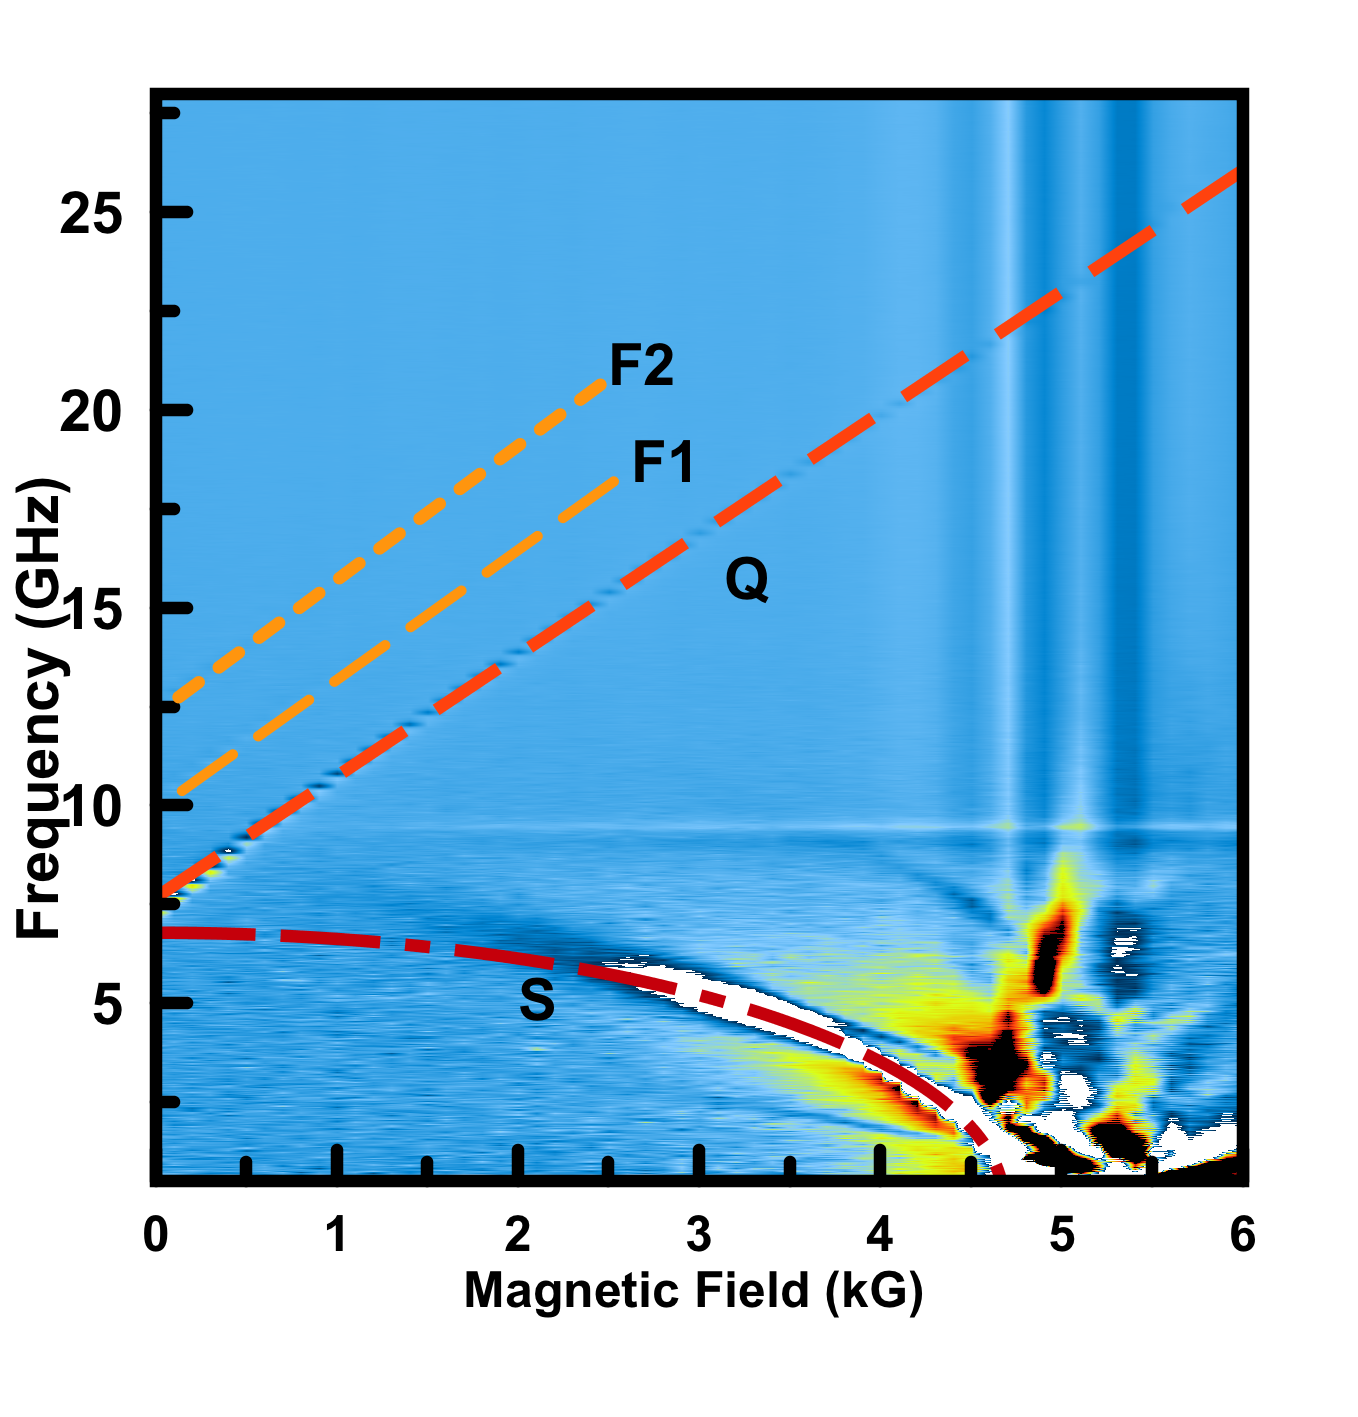
\includegraphics[width=0.8\textwidth]{fig/FieldMod/contour.png}
  \centering
  \caption{ST-FMR spectra measured as a function of out-of-plane magnetic field. Q labels the quasi-uniform mode of the free layer while F2 and F3 are the higher order spin wave modes of the free layer. S labels the acoustic SAF mode. }
  \label{fig:2D}
\end{figure}


When we have the resonant coupling between these two modes, the linewidth would be broadened by this resonant coupling mechanism. This is exactly what we have found from Fig.\ref{fig:2D} in the lower frequency region.

In the 2D contour plot, around 4kG magnetic field, as we can see from Fig.\ref{fig:d}, the SAF layer becomes unstable and enter the spin-flop region. In this region, because of unstable SAF layer, the stray field from SAF layer acting on the free layer is also very unstable and produce large magnetic noise during the ST-FMR measurement. As a result, we find there are more fluctuations in the linewidth data as we see from Fig.\ref{fig:LW} around 20GHz.

As we have learned from the 2D contour plot, in order to reliably fit for the damping parameter in the free layer, we need to first exclude the resonant coupling region in the lower frequency, in which the linewidth was broadened by the interaction between free and SAF layer. We also need to avoid the high frequency region. In Fig.\ref{fig:LW_FIT} we only include the linewidth data from 10GHz to 20GHz and determine the Gilbert damping to be 0.007 from the slope.
 
\begin{figure}[h]
  \centering
  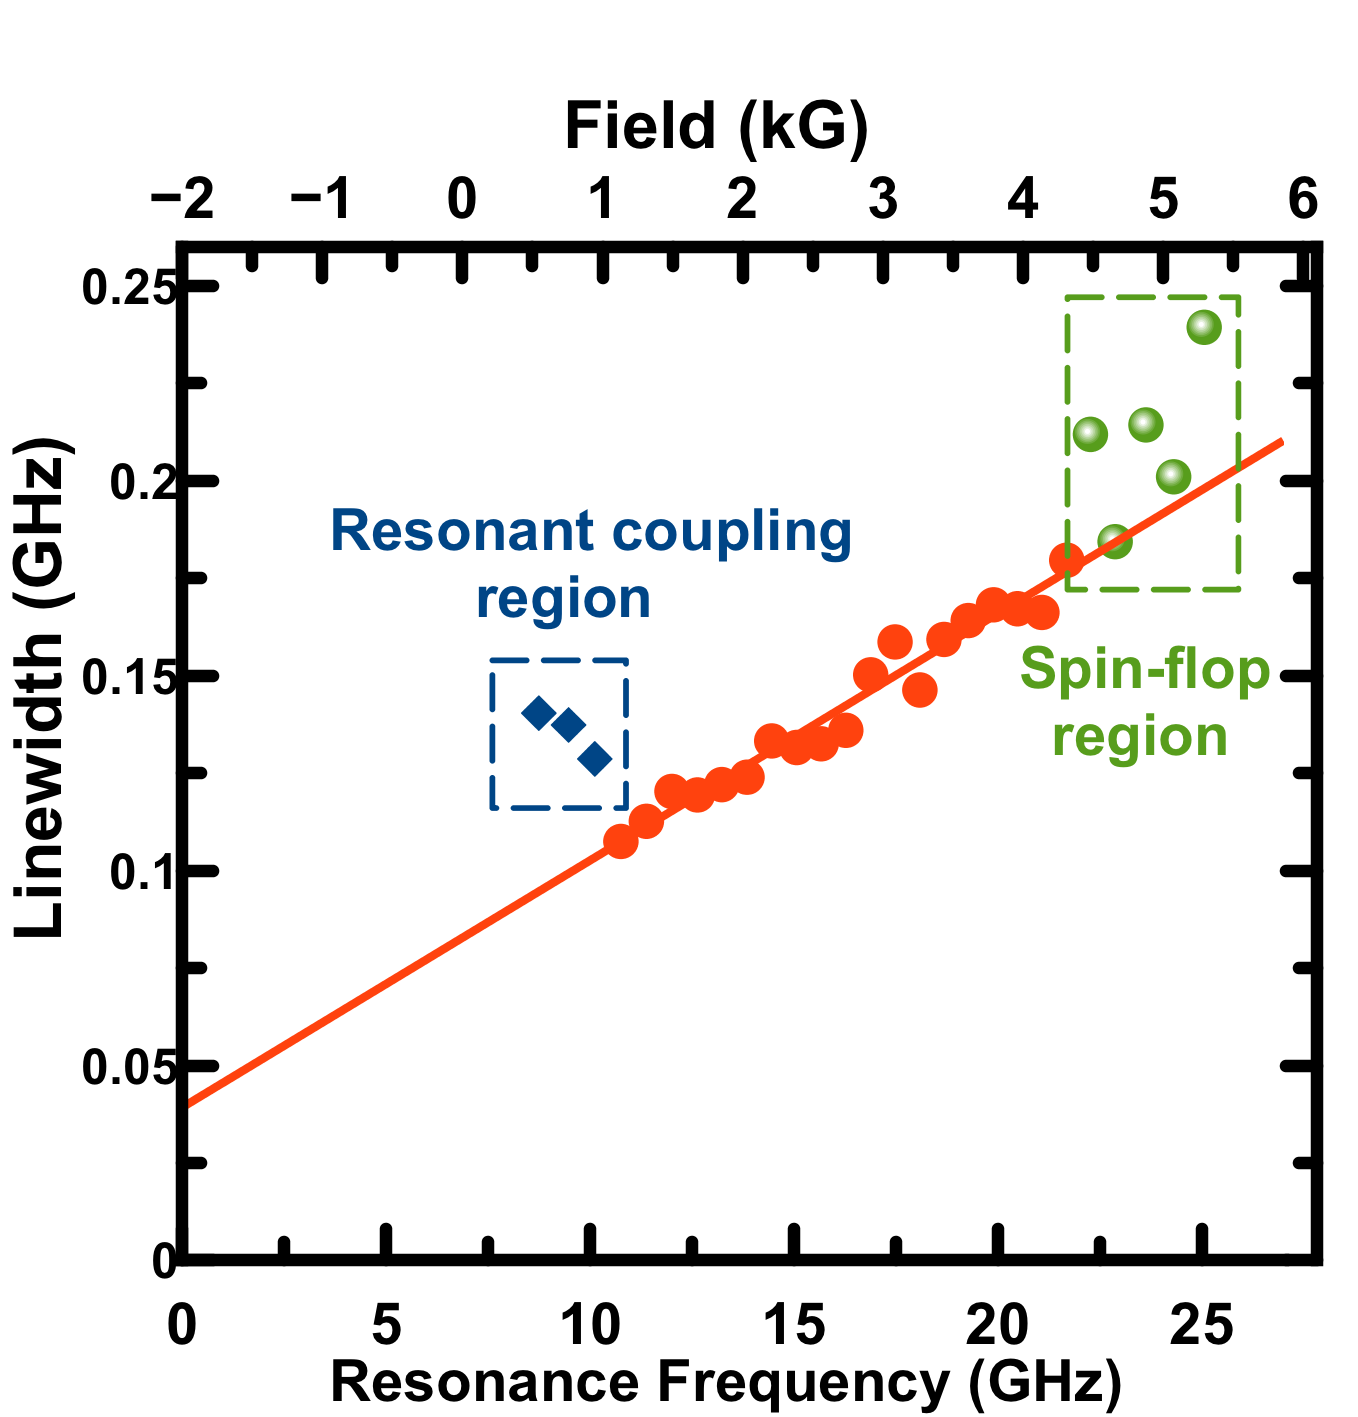
\includegraphics[width=0.8\textwidth]{fig/FieldMod/LW_PLOT.png}
  \caption{Spectral linewidth of the free layer quasi-uniform mode versus frequency of the mode. Line is the best fit to the data outside of the SAF spin flop and SAF resonant coupling regions.}
  \label{fig:LW_FIT}
\end{figure}

Here the intercept $\Delta f_0$ is linewidth at zero resonance frequency, which is often due to inhomogeneous effects such as the dispersion in effective anisotropy field from the distributions of demagnetization field and stray field\cite{inhom}. From the fitting of the slope, we obtain a low Gilbert damping value around 0.006, which is consistent with other measured Gilbert damping value for the CoFeB-based free layer in similar work\cite{STFMR_1}. Such a small value of Gilbert damping is essential for lowering critical switching voltage as we previously discussed. The critical switching voltage given by Eq.\ref{eq:criticalV} is 0.85 V. From the intercept at zero resonance frequency, we obtained the intercept $\Delta f_0$ around 0.0392 GHz. We would like to further investigate the non-zero intercept and the inhomogeneity in the free layer of the MTJs by micromagnetic simulations.








\section{Continous wave Micromagnetic Simulations}

To understand the linewidth and nature of non-intercept intercept we observed, we perform continuous wave micromagnetic simulations of magnetization dynamics using OOMMF software\cite{OOMMF}. To fully account the magnetic dynamics in all layers, we employ a three-dimensional with three ferromagnetic layers: free, SAF top and SAF bottom. We use material parameters obtained from independent measurements and/or their accepted literature values. The cell size used is 0.25 nm, which is comparable to the grain size observed in the CoFeB system\cite{grain}. 

\begin{figure}[h]
  \centering
  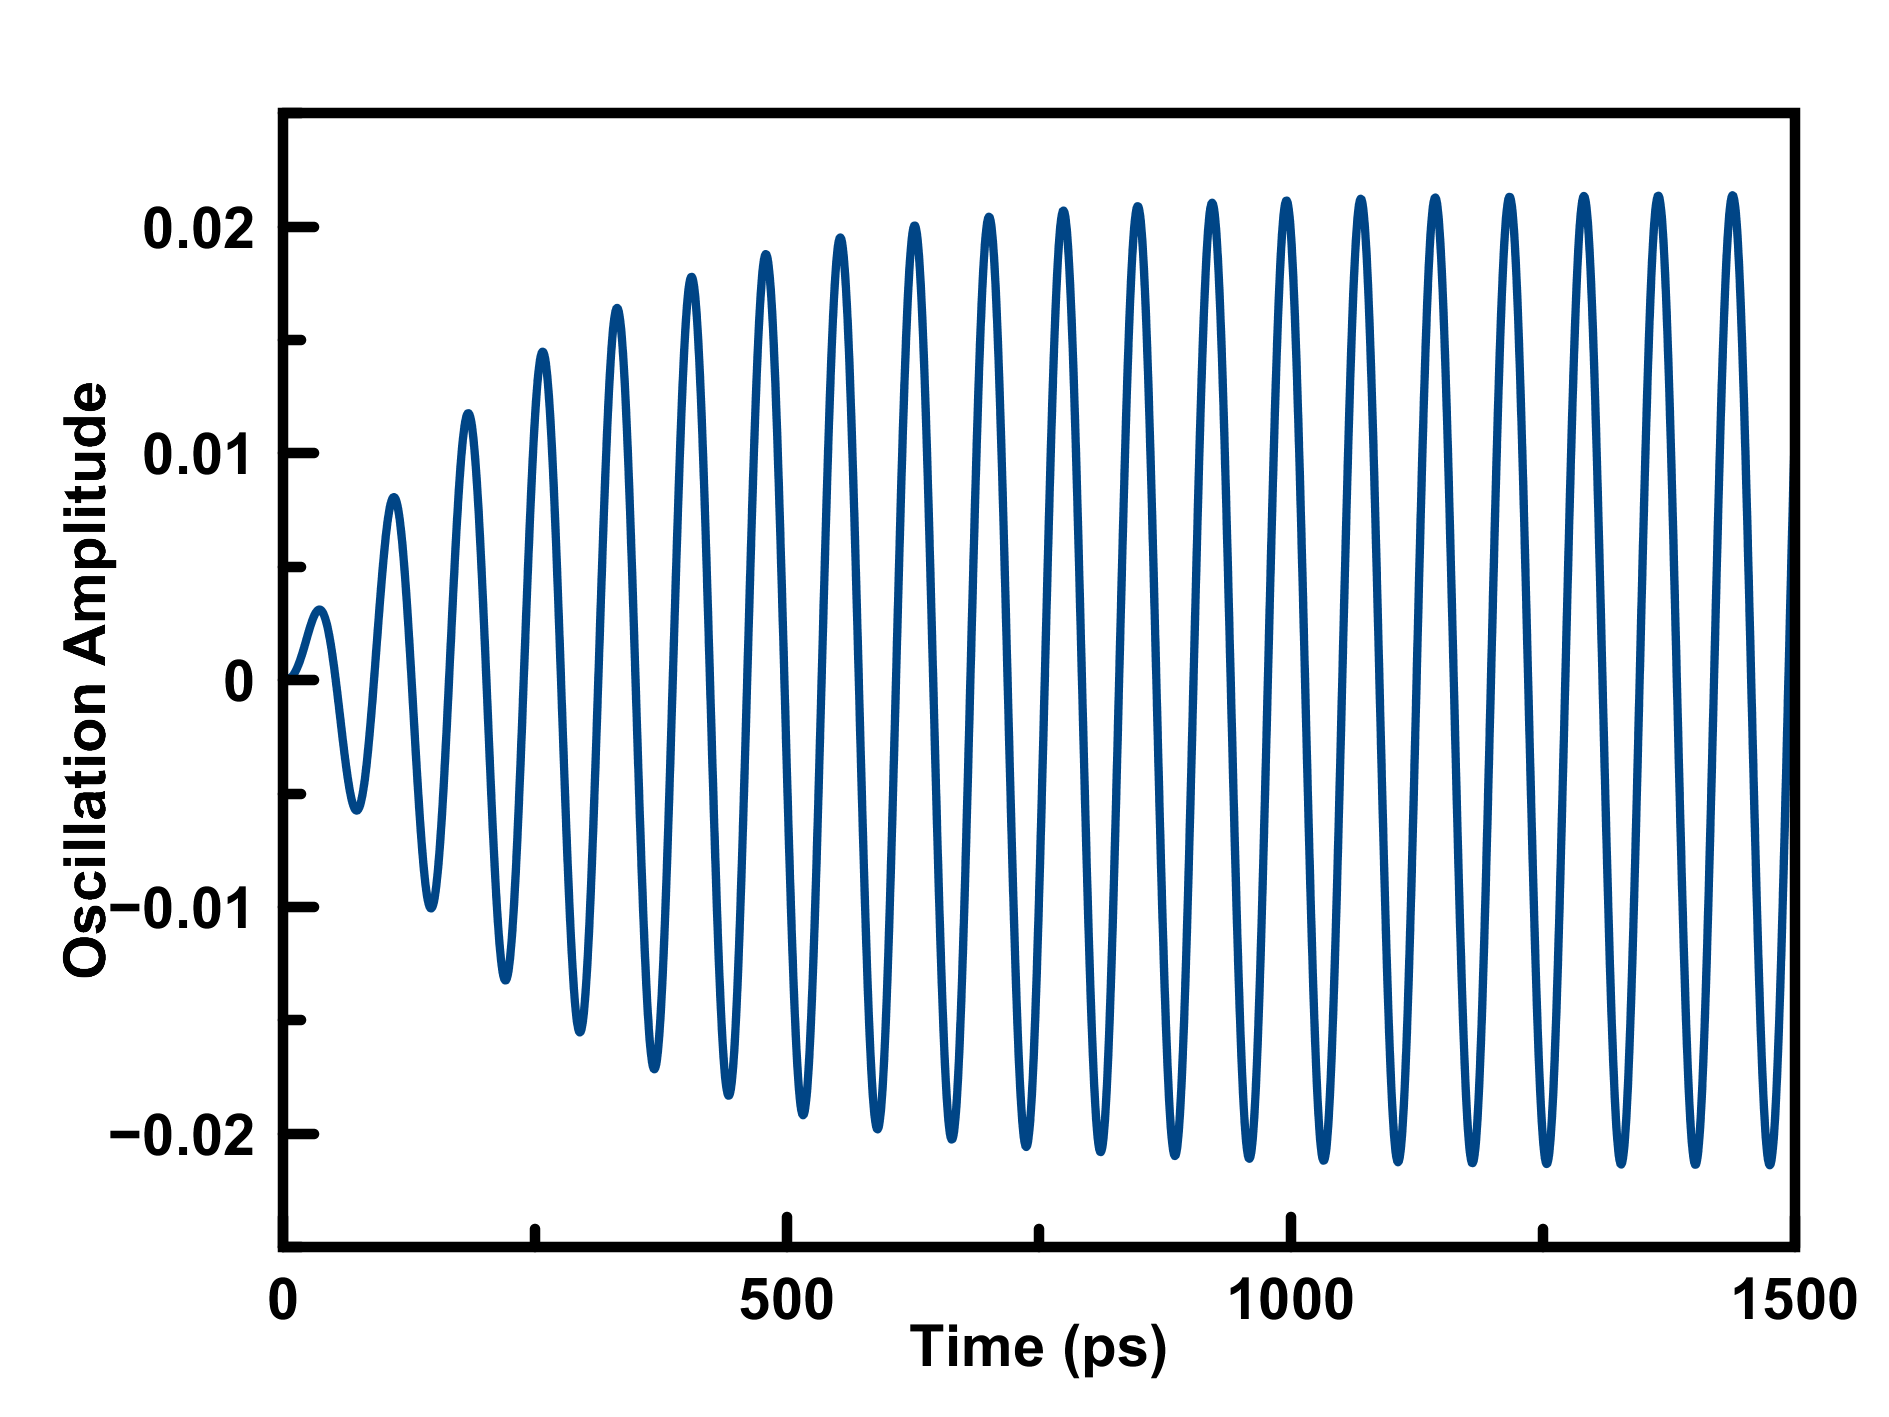
\includegraphics[width=0.6\textwidth]{fig/Time_oscillation.png}
  \caption{Spectral linewidth of the free layer quasi-uniform mode versus frequency of the mode. Line is the best fit to the data outside of the SAF spin flop and SAF resonant coupling regions.}
  \label{fig:timeOscilation}
\end{figure}

In the simulations, the spin wave dynamics is excited by a combined pulse of spin-torque and Oersted field, both resulting from a sine-wave-driven current. During the simulation process, we first relax the system under static magnetic field to reach the ground state. Then the magnetization is excited by sine-wave drive and oscillate with increasing amplitude. After a certain period of transient time, the magnetization will precess steadily and enter dynamic equilibrium. To illustrate this process, we can plot the magnetization as a function of simulation time as shown in Fig.\ref{fig:timeOscilation}. The magnetization first undergoes a period of transient time and then enter a steady oscillations, which yields a certain value of oscillation amplitude and phase. For each driven frequency, we can determine corresponding amplitude of the oscillation at a constant magnetic field. The blue dot from Fig.\ref{fig:Sim_spectrum} show the oscillation amplitude of the in-plane component of magnetization as a function of applied  frequency at 2000 Oe field, which shows a typical Lorentzian curve as expected\cite{Tulapurkar2005}. From the simulation, We can adjust the perpendicular uniaxial anisotropy in order to reproduce the same experimental resonance frequency(7.54 GHz) at zero magnetic fields. The fitted uniaxial anisotropy  is $4.05 \times 10^5 J/ m^3$. Compared with the magnetic anisotropy field we measured from field-modulated ST-FMR methods, we can also calculate the perpendicular uniaxial anisotropy field from the following equation \cite{Ohno2010}

\begin{equation}\label{eq:hk}
H_k = 2 K_u /M_ s - 4 \pi M_s . 
\end{equation}


Here $H_k$ is the effective magnetic anisotropy, $K_u$ is the uniaxial perpendicular magnetic anisotropy and $M_s$ is the saturation magnetization. The PMA calculated from experimental value is $4.73 \times 10^5 J/ m^3$, which has around 15\% deviation from micromagnetic simulated value. This discrepancy in the magnetic anisotropy shows the deviations between the macrospin Kittel equation and the simulated micromagnetic model.  


\begin{figure*}[t]
\centering     
\subfigure{\label{fig:uniform_spectrum}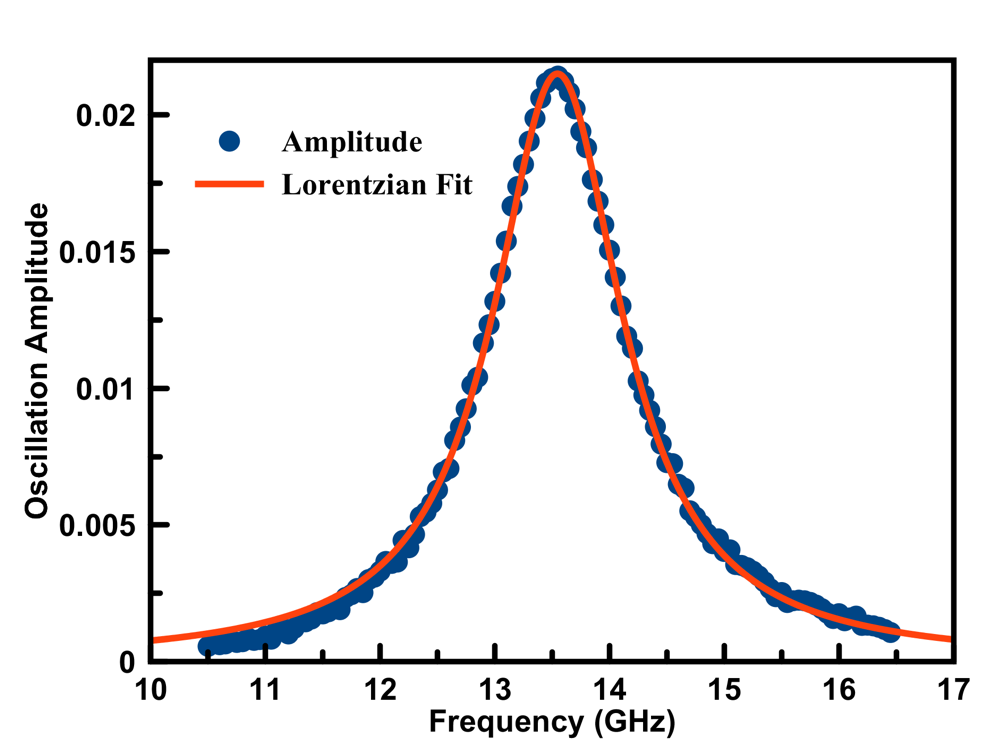
\includegraphics[width=70mm]{fig/CW_sim/uniform_spectrum.png}}
\subfigure{\label{fig:uniform_mode_profile}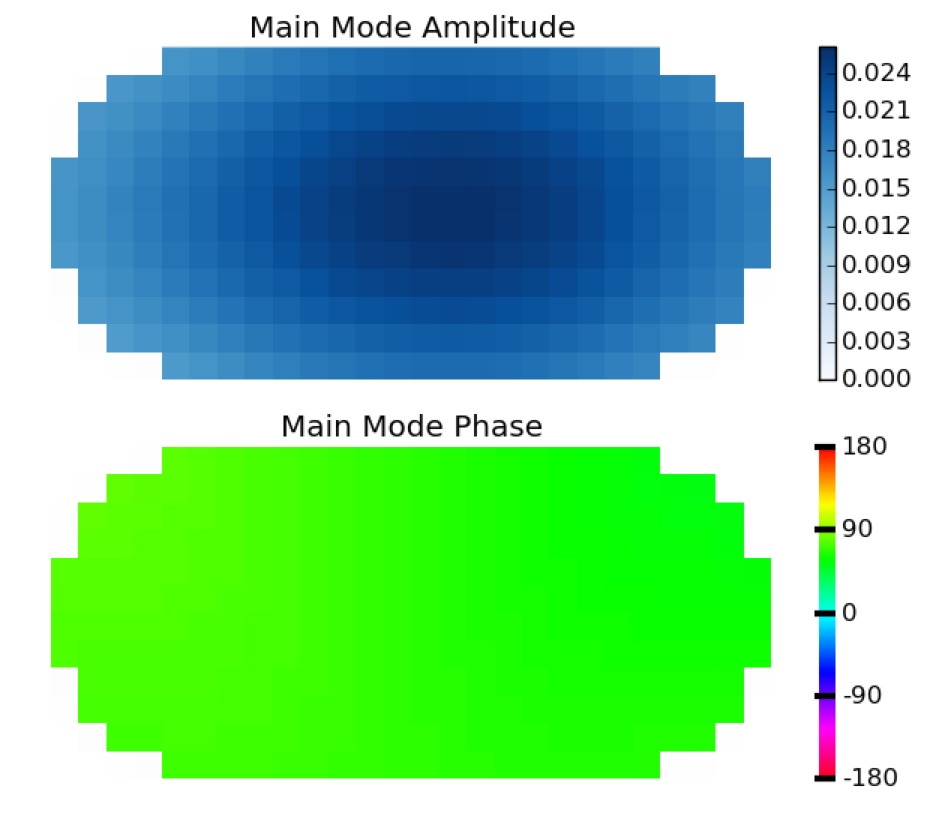
\includegraphics[width=70mm]{fig/CW_sim/mode_profile_1.png}}
\caption{(a)Blue dot: Simulated amplitude versus driven frequency. Red line: Fitted Lorentizan curve. (b)Spatial profile of mode amplitude(Top) and phase(Bottom) of the mode excited in the continuous wave. The amplitude and phase are both uniform across the device, indicating a quasi-uniform eigenmode. }
\end{figure*}


Let us now focus the simulated linewidth from this continuous wave simulations. In this type of simulation, we adopt the Gilbert damping value of 0.05 to avoid longer relaxation and simulation time. By simulating the spectrum at the different magnetic field, we can also fit for the resonance frequency and linewidth as we have done experimentally in Fig.\ref{fig:LW}. The blue dot and dashed line in Fig.\ref{fig:uniform_lw} shows such data from this simulation. The fitted  Gilbert damping constant $\alpha$ is 0.05 with an intercept at zero frequency $\Delta f_0$ 0.002, which shows that at this perfectly uniform model, the inhomogeneous broadening should be really weak and the $\Delta f_0$ should be close to zero. We find that this type of finite cell simulation does not introduce a large non-zero intercept at zero frequency as we observed from the experiment.

\begin{figure}[h]
  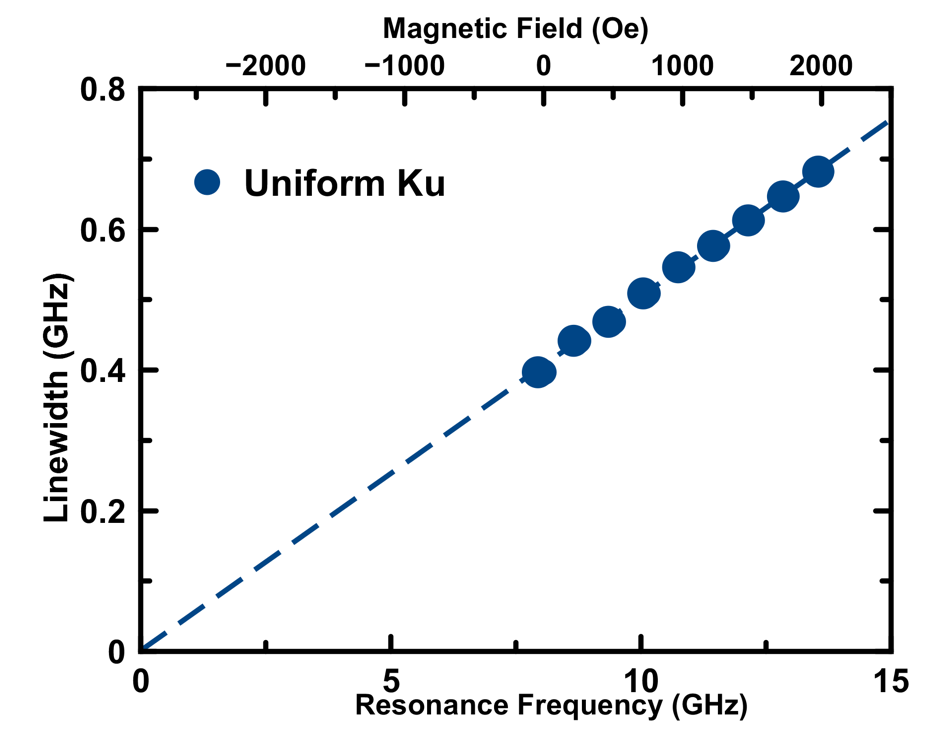
\includegraphics[width=0.6\textwidth]{fig/CW_sim/uniform_LW.png}
  \centering
  \caption{ST-FMR spectra measured as a function of out-of-plane magnetic field. Q labels the quasi-uniform mode of the free layer while F2 and F3 are the higher order spin wave modes of the free layer. S labels the acoustic SAF mode. }
  \label{fig:uniform_lw}
\end{figure}

In the next step of the micromagnetic simulation, we introduce a random anisotropy field that varies spatially. The perpendicular uniaxial anisotropy value at the micromagnetic cell is drawn uniformly from the minimum and the maximum value, which are $3.55 \times 10^5 J/ m^3 $ and  $4.55 \times 10^5 J/ m^3 $ respectively. This variation in the perpendicular uniaxial anisotropy corresponding to the effective magnetic anisotropy to range from in-plane direction 0.1 kG to perpendicular direction 0.21 kG in the simulations(assuming uniform magnetizations across the free layer). We can then repeat the simulation procedure as described above. The red dot and fitted curve at Fig. \ref{fig:random_spectrum} shows the amplitude versus frequency response with this anisotropy fluctuations. Now we still have a Lorentzian curve with some extra noise, which is due to the randomness of anisotropy introduced in the free layer. We can still look at the mode amplitude and phase, as shown in Fig.\ref{fig:random_mode_profile}. Compared with Fig.\ref{fig:uniform_mode_profile} we start to some deviations from uniform excitations, with nodes along the edges. Fig.\ref{fig:Hk_dist} shows the spatial distributions of the random anisotropy across the sample. We can also plot the linewidth as a function of resonance frequency as shown in the green dot in Fig.\ref{fig:CW_lw_summary}. The fitted Gilbert damping value is 0.051 with a intercept -0.0027 GHz. From here we can conclude that only introducing random fluctuations of anisotropy does not reproduce the experimental intercept value.




In the final step of the simulation, we decrease the exchange constant between each grain from 20 pJ/m to  5 pJ/m. We can also plot the linewidth versus frequency as it is shown in the red dot from Fig.\ref{fig:CW_lw_summary}. The slope of this green line gives a Gilbert damping value of 0.04733, which is slightly different from the input damping value. Most importantly, the intercept  at zero frequency $\Delta f_0$ is broadened to  0.043. This value is indeed close to our experimentally determined $\Delta f_0$, 0.0392.  

\begin{figure*}[t]
\centering     
\subfigure{\label{fig:random_spectrum}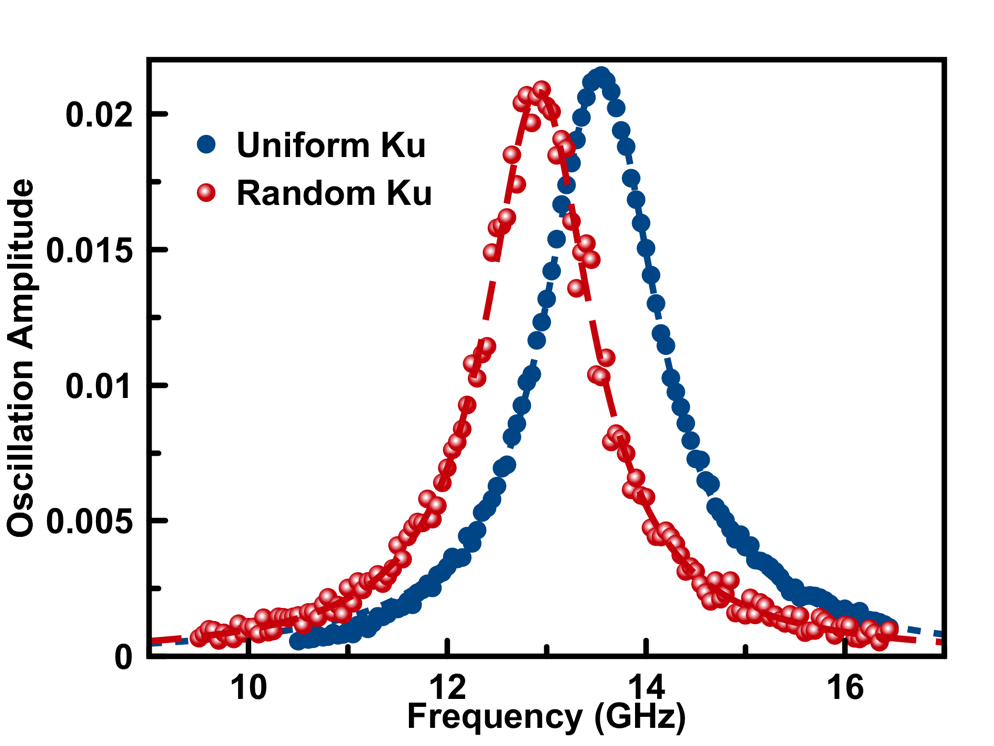
\includegraphics[width=50mm]{fig/CW_sim/random_spectrum.png}}
\subfigure{\label{fig:random_mode_profile}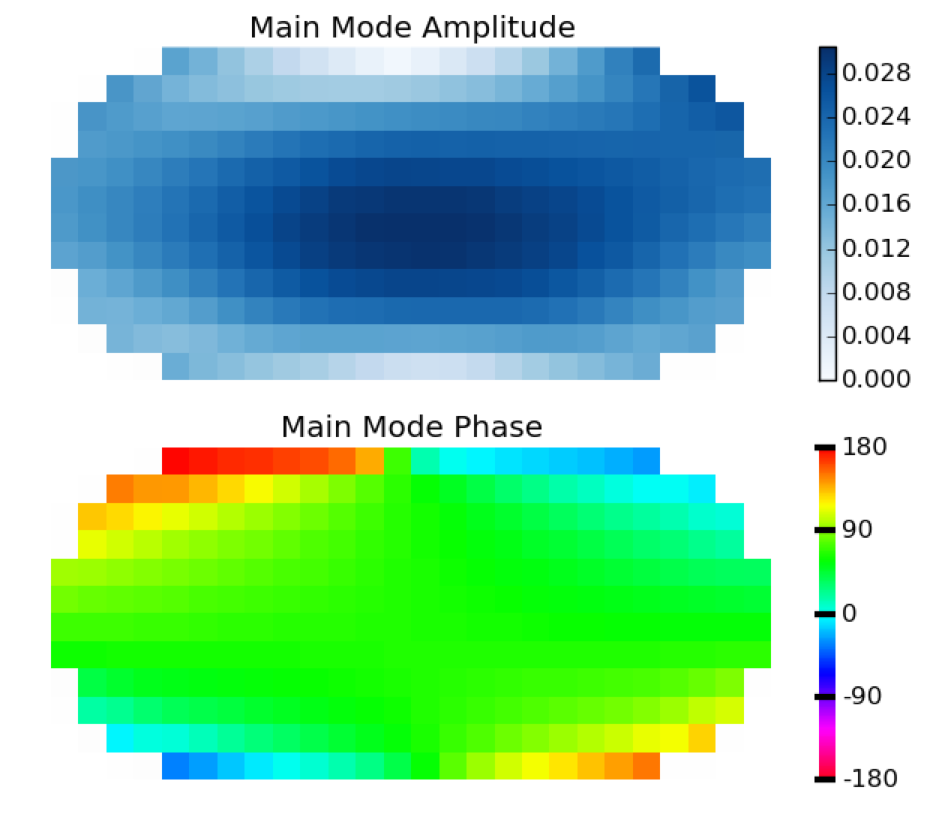
\includegraphics[width=50mm]{fig/CW_sim/mode_profile_2.png}}
\subfigure{\label{fig:Hk_dist}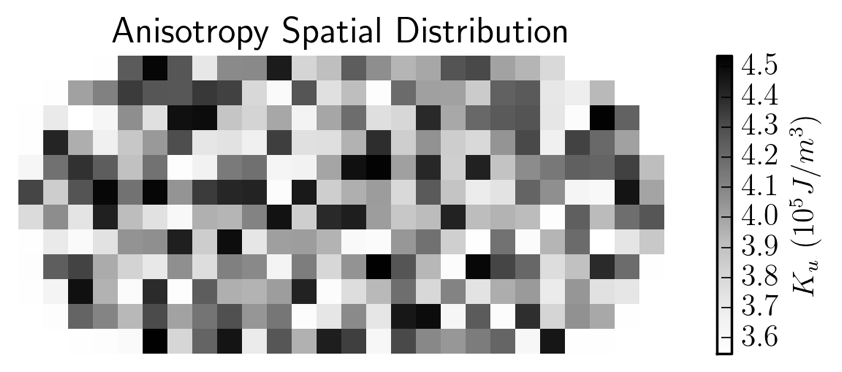
\includegraphics[width=50mm]{fig/CW_sim/Kudist.png}}
\caption{(a).Simulated spectrum with random magnetic anisotropy(in red dot) compared with spectrum with uniform magnetic anisotropy(blue dot) (b) Top: Spatial profile of the mode amplitude excited. Bottom: Spatial profile of the mode phase. (c)Spatial distributions of the magnetic anisotropy when introducing the random distributed magnetic anisotropy in OOMMF.}
\end{figure*}


In fact, since the CoFeB free layer is composed of grains, each with slightly different anisotropy, with strong exchange coupling inside of the grain and weaker exchange coupling among the grains\cite{grain}. In our simulation, by introducing random anisotropy field and decreasing the exchange stiffness with micromagnetic cell size close to the typical grain size of the CoFe crystals, we are reproducing the locally variant anisotropy field among the free layer, which contributes to the non-zero intercept $\Delta f_0$ we observed from previous ST-FMR measurement. Thus, we can qualitatively quantify the degree of random fluctuations of the magnetic anisotropy in the free layer of the MTJs.  



\begin{figure}[h!]
  \centering
  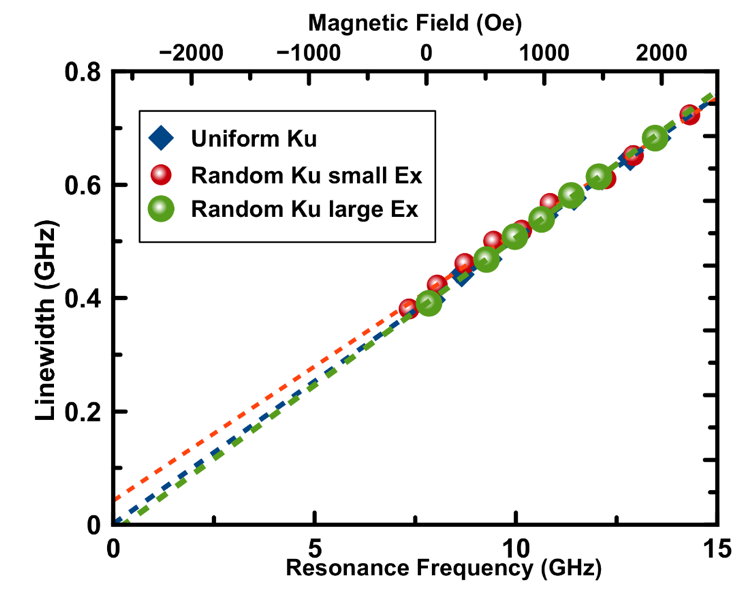
\includegraphics[width=0.8\textwidth]{fig/CW_sim/LW_summary.png}
  \caption{Summary of simulated linewidth plotted versus resonance frequency with different material parameters. From the plot only random magnetic anisotropy combined with small exchange stiffness leads to a significant linewidth intercept at zero resonance frequency.}
  \label{fig:CW_lw_summary}
\end{figure}


\begin{table}[h!]
\centering
 \begin{tabular}{||c c c||} 
 \hline
  & Gilbert damping $\alpha$  & Intercept $\Delta f_0$\\ [2.0ex] 
 \hline\hline
 Uniform
Uniform  & 0.05 & 0.0016$\pm$0.0064  \\ 
 \hline
 Random Ku with small Ex  & 0.047 & 0.043 $\pm$0.013 \\
 \hline
 Random Ku with large Ex  & 0.051 & -0.0027$\pm$0.0088  \\
 \hline
\end{tabular}
\caption{Table to test captions and labels}
\label{table:summary_LW}
\end{table}

We can summarize the simulation results from Table\ref{table:summary_LW}. It is clear that only combining low exchange stiffness with random fluctuations of magnetic anisotropy would lead to linewidth broadening at zero resonance frequency.

\newpage
\section{Micromagnetic Simulations}
In order to fully understand the magnetic dynamics being excited in the Magnetic Tunnel Junctions, we perform micromagnetic simulations using OOMMF package\cite{OOMMF}. To fully account for all magnetic interactions in the MTJ, we use a three dimensional model with three main functional layers: free layer, SAF top and SAF bottom layer. In the simulation, spin wave dynamics is excited by a combined pulse of ST and Oersted field, both resulting from a sinc-shaped spatially uniform current pulse with the amplitude $J_{C}\frac{\sin(2\pi f_{c} t^{'})}{2\pi f_{c}t^{'}} $ with the amplitude the cut-off frequency around 20 GHz, and the time variable $t_{0}$ 500 ps. The need to combine the excitation from Spin torque and Oersted field is to include the uniform and non-uniform spin wave modes in the MTJs\cite{Modes}.
The spatial profile of the Oersted field is assumed to be that of a long wire with elliptical cross section. The direction of the ST vector acting on the free layer is determined by the magnetization orientation of the SAF top layer.Spectrum of spin wave eigenmodes is obtained via the Fast-Fourier-transform (FFT) of the time dependent in-plane component of the MTJ net magnetic moment. 




\begin{figure}[!ht]
\centering
\subfigure{\label{fig:MR18}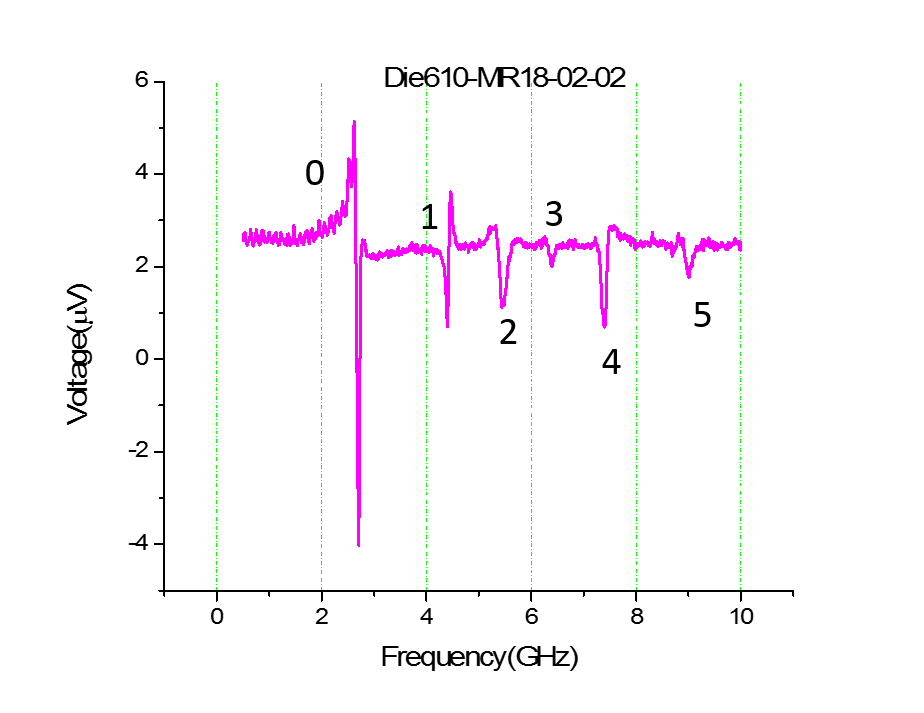
\includegraphics[width=75mm]{fig/MR18.png}}
\subfigure{\label{fig:Simulation}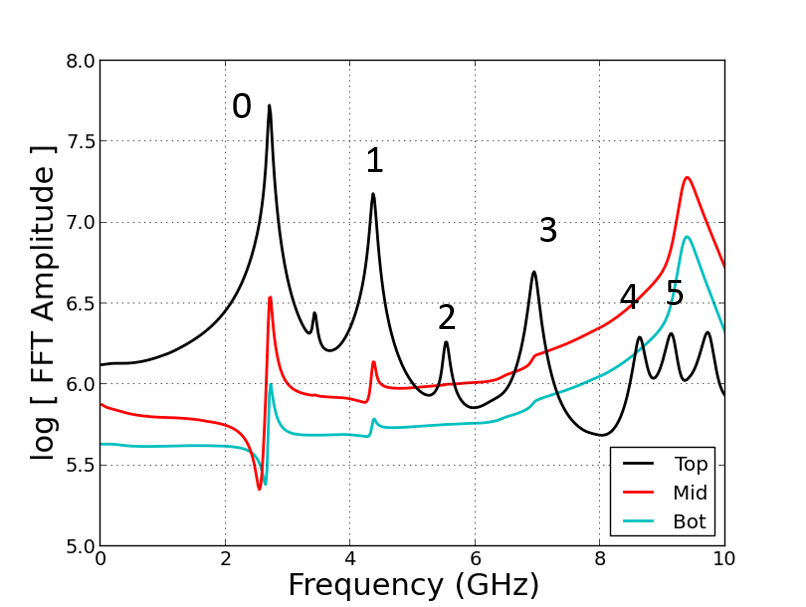
\includegraphics[width=75mm]{fig/simulation.png}}
\caption{(a) ST-FMR spectrum of a 30 nm by 150 nm stadium-shaped STT-MRAM element. Several spin wave eignemode resonances are seen in the spectrum. (b)Fitted spectrum from micromagnetic simluations.}
\end{figure}

Fig.\ref{fig:MR18} shows a typical ST-FMR spectrum from our measurement. For this sample, we can identify five spin wave modes. The zero mode is the uniform excitation and we have already used this mode to fit for magnetic anisotropy and Gilbert damping value. The other four modes are non-uniform modes excited along the edges. On the left, Fig.\ref{fig:Simulation} shows the simulated spectrum from our micromagnetic calculations. As we discussed before, we perform the Fast-Fourier-transform on the in-plane component of the MTJ net magnetic moment and plot it against driven frequency. The top layer is the free layer and the middle(bottom) is the SAFTop(SAFBottom) layer. As we can see from the plot, the amplitude of the top layer is definitely much larger than the other layers, meaning the excitation of the MTJs is dominant by the free layer. The peaks in the spectrum are corresponding to the spin wave modes we observe from the experiment. By tuning the material parameter such as magnetic anisotropy and exchange constant, we can match the frequency position of the first zero mode and the second mode. So firstly, from micromagnetic simulations, we can determine the magnetic anisotropy to be $3.13*10^5 J/m^3$ and exchange stiffness constant to be around $5*10^{-12} J/m$.

Next we would like to understand the nature of the modes we excited. To do this, we perform the spatial mapping of the mode amplitude and plot it in Fig.\ref{fig:mode}. Starting from the top left, we list the model profile for all the five modes. As expected, the first mode is uniform excitation so the amplitude of this mode is uniform. The second mode has two nodes along the short axis. So we label it as Mode(2,0). Then we have modes from Mode(3,0) and Mode(4,0) which have three or four nodes along the short axis. The last mode has one node along the long axis, so it is labeled as Mode(0,1).





\begin{figure}[h!]
  \centering
  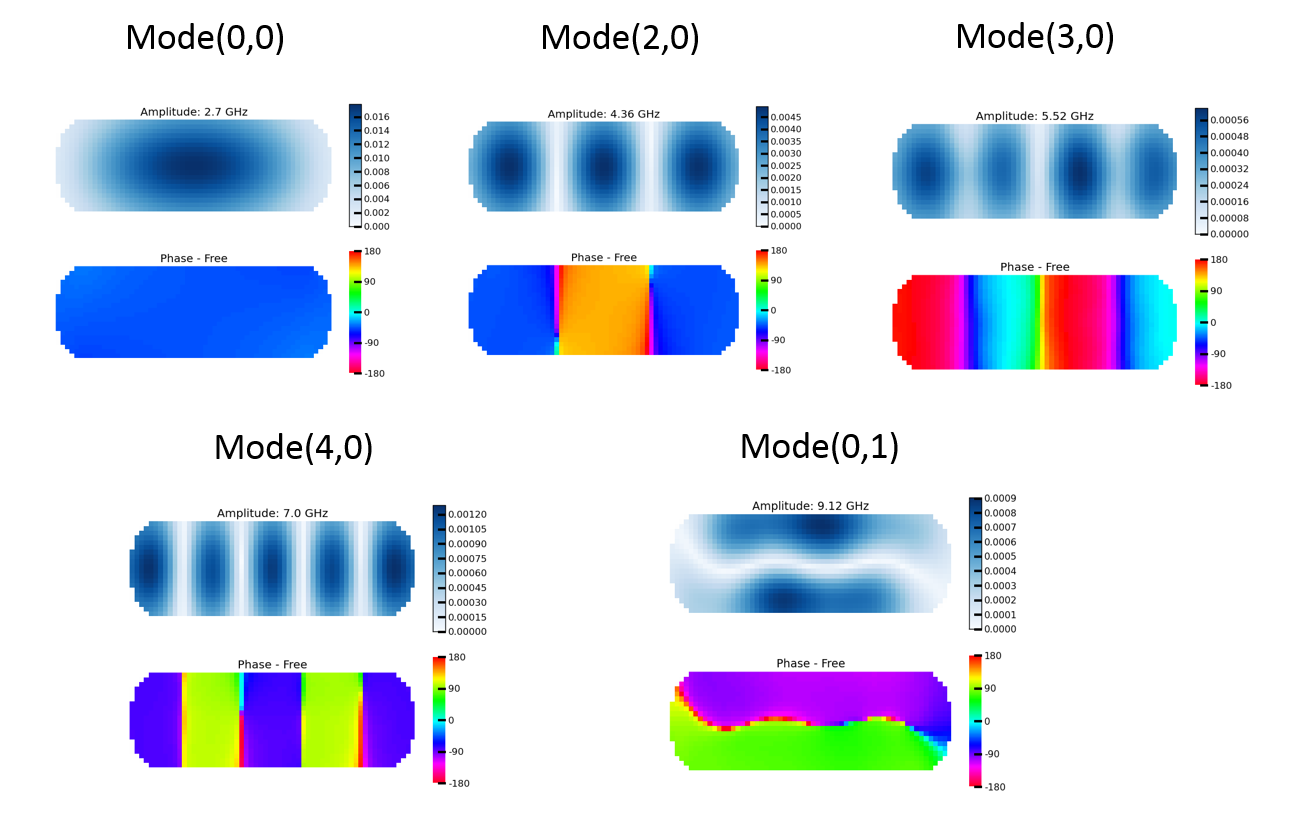
\includegraphics[width=1.0\textwidth]{fig/Mode_pic.png}
   \caption{Spatial mapping of modes excited in the micromagnetic simulations. }
  \label{fig:mode}
\end{figure}

After that, we find that no matter how we tune the magnetic anisotropy and exchange constant, the latter three modes can not be matched very well from experiment and simulations. So we have to consider another possibilities. One thing to consider is magnetic edge damage of the MTJ element. Such modifications are unavoidable in the STT-MRAM fabrication process due to etching of the element, and they are predicted to have significant impact on current-driven switching of the free layer. We tested several micromagnetic models of the magnetic edge damage and found how these models modify the frequencies of spin wave eignemodes. We then compared the  model’s predictions to our measurments of spin wave spectra by spin torque ferromagnetic resonance. This comparison allowed us to determine which model best describes the experimental data. More specifically, we have tested three models of the magnetic edge damage: 

-	Magnetic dilution model. In this model, saturation magnetization and exchange stiffness of the free layer of STT-MRAM are reduced in the edge region.
-	STT-MRAM shape distortion model. In this model, the MTJ nanopillar shape is distorted with respect to its nominal shape.
-	Anisotropy reduction model. In this model, magnetic shape anisotropy is reduced near the sample edges.

Fig.\ref{fig:edge_damage} shows the results by exploiting edge damage model in the simulation. From this plot we find that this mode cannot adequately describe the experimentally observed spectrum of spin wave eignemodes in STT-MRAM samples we experimentally studied. Compared with the edge anisotropy model in Fig.\ref{fig:edge_ani}, now we have a much better agreement between experiment and simulations. We, therefore, conclude that the major impact of the STT-MRAM edge on magnetic properties of the device is reduction of perpendicular magnetic anisotropy near the device edge. This reduction can result in nucleation of current-driven magnetization reversal near the sample edges  Comparison of ST-FMR measurements of spin wave mode frequencies can quantify the degree of magnetic anisotropy reduction near the sample edges. We discuss how this can be accomplished in the next paragraph. 

\begin{figure}[!ht]
\centering
\subfigure{\label{fig:edge_damage}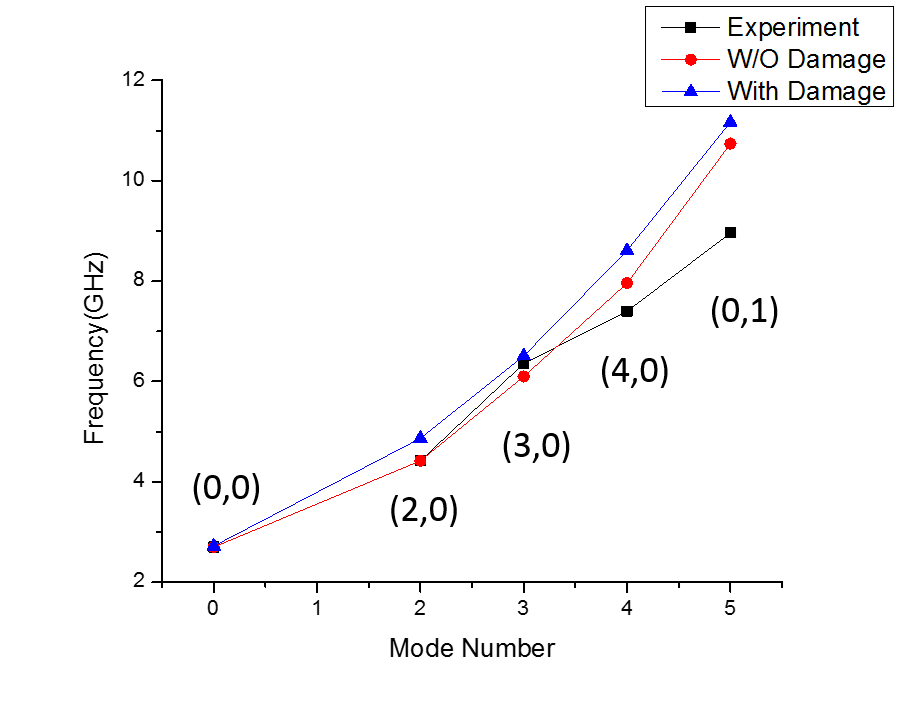
\includegraphics[width=80mm]{fig/edge_damage.png}}
\subfigure{\label{fig:edge_ani}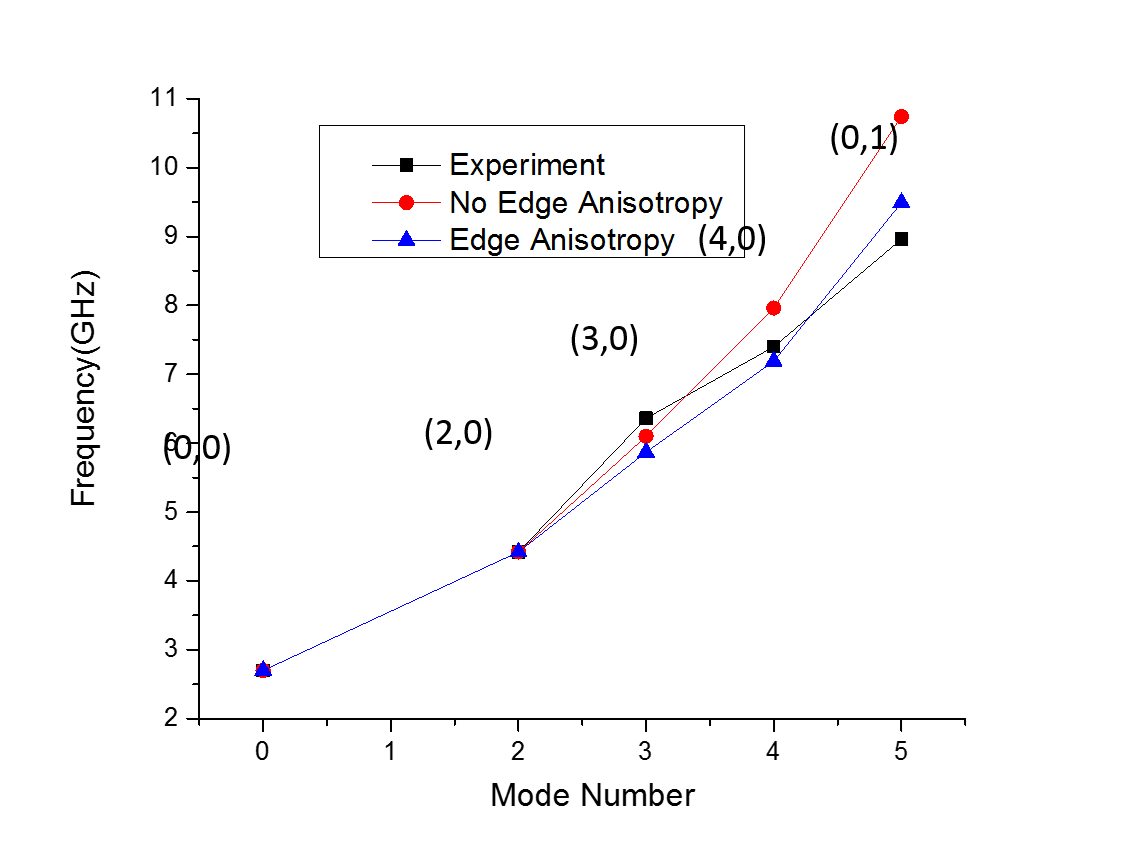
\includegraphics[width=80mm]{fig/edge_ani.png}}
\caption{(a) ST-FMR spectrum of a 30 nm by 150 nm stadium-shaped STT-MRAM element. Several spin wave eignemode resonances are seen in the spectrum. (b)Fitted spectrum from micromagnetic simluations.}
\end{figure}

From fitting the first and second mode frequencies, we already have a confidence value of magnetic anisotropy and exchange constant. Then we employ the models of spatially non-uniform parameters of the free layer. The blue symbols in the left panel of Fig.\ref{fig:edge_damage} show results of the simulations for the magnetic edge dilution model. In this model, both the saturation magnetization and the exchange constant of the free layer are gradually reduced from their bulk values to zero at the free layer edge. The distance over which this reduction takes place was chosen to be in the 2.5 nm to 7.5 nm range (typical material damage depths due to various types of etching). It is clear from Fig.\ref{fig:edge_damage} that the magnetic dilution model does not improve the agreement between theory and experiment. We have also found that shape distortions of the free layer do not reproduce the experimental results well. In contrast, reduction of magnetic anisotropy from  $3.13*10^5 J/m^3$ in the free layer interior to $3.03*10^5 J/m^3$ at the free layer edge over a distance of 2.5 nm gives a much better agreement with the experimental data as shown by blue symbols in the Fig.\ref{fig:edge_ani}. This type of fitting allows us to obtain the exchange stiffness constant of the free layer, its perpendicular magnetic anisotropy value and the magnitude of reduction of the perpendicular anisotropy at the sample edge.















\section{Circular STT-MRAM Devices with Broken Symmetry}

While stadium-shaped or rectangular samples are convenient for studies of the edge damage due to their particularly simple spin mode structure, studies of circular STT-MRAM samples are important because this shape is the primary candidate for STT-MRAM. We performed ST-FMR measurements of circular STT-MRAM samples and measured their spin wave spectra as a function of the nanopillar diameter. Fig.\ref{fig:circularmode} shows two examples of such spectra for STT-MRAM cells with diameters of 250 nm and 80 nm measured as a function of out-of-plane magnetic field. A large number of modes are observed for the 250 nm sample due to the relatively weak geometric confinement of spin waves in the large structure. For these larger devices, it would be relatively hard to identify all the modes excited. While you can still fit for some of the spin-wave modes, the frequency spacings between each mode is relatively small, which makes further quantitatively analysis.
 
 \begin{figure}[h!]
  \centering
  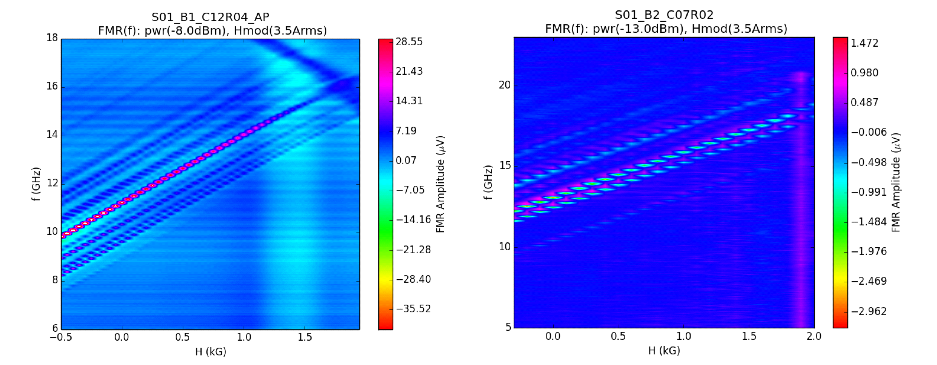
\includegraphics[width=1\textwidth]{fig/FieldMod/ap-p.png}
   \caption{ST-FMR spectra of circular STT-MRAM cells with 250 nm diameter (left) and 80 nm diameter (right) measured as a function of the out-of-plane magnetic field applied to the nanopillar.}
  \label{fig:apandp}
\end{figure}

When we move to much smaller devices, fewer spin wave modes with larger inter-mode frequency gaps are seen for the 80 nm sample. The spin wave mode structure in circular STT-MRAM samples is qualitatively different from that in the stadium-shaped samples. The modes are characterized by two indexes: n = (0, 1, 2…) and L = (0,1)\cite{excitation2}. The index n gives the number of spin wave nodes in the radial direction, while the index L describes azimuthal phase variation of the mode. Spatial profiles of the three lowest-frequency modes in a perfectly circular sample with 60 nm diameter are shown in Fig. \ref{fig:circularmode}. The first mode(labelled as (0,0)) is the lowest-frequency quasi-uniform mode. The second mode(labelled as (0,1)) is the first higher-order mode, it has larger amplitude at the edges and a node at the center. The last mode in \ref{fig:circularmode} is labelled as (1,0), which has a node along the edges of the device. This is the case when we have a perfect circular shape MRAM sample.
 
\begin{figure}[h!]
  \centering
  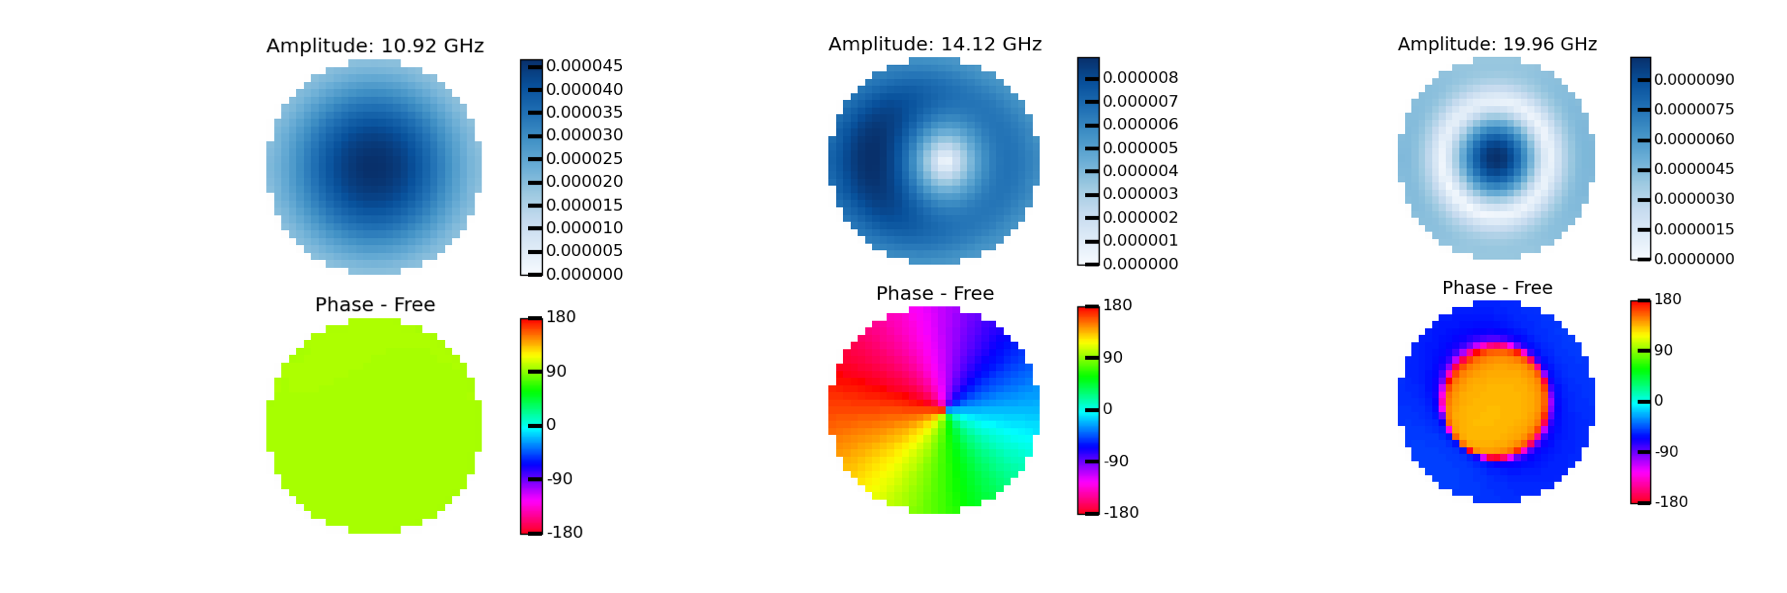
\includegraphics[width=0.8\textwidth]{fig/FieldMod/mode-profile.png}
   \caption{Three lowest-frequency spin wave eigenmodes of the free layer of a circular STT-MRAM sample with 60 nm diameter. The top image shows the spatial map of the amplitude of the mode while the bottom image shows the spatial map of the spin wave mode’s phase}
  \label{fig:circularmode}
\end{figure}


However, in our experimental data, we find the frequency of the second higher-order mode(label as mode(0,1)) is considerably larger than micromagnetic simulations. To  confirm this finding, we measured more than ten MRAM devices with the same nominal dimension. The ST-FMR spectra of all circular samples we studied exhibit one common feature: the lowest frequency (quasi-uniform) mode always appears as a singlet while the two higher frequency modes appear as a doublet with relatively small inter-mode frequency splitting (~ 1GHz). Furthermore, we find there is a distribution of all the three modes frequencies. Fig.\ref{fig:stat1} summarizes the experimental results, which shows the statistics of the mode frequencies at zero field for different modes. We find that the distribution is somewhat skewed towards lower frequencies. We also notice that there is a clear visibly larger spread for the (1,0) and (0,1) modes compared to the (0,0) mode. This is because the (1,0) and (0,1) mode frequencies are also affected by random in-plane anisotropy fluctuations due to e.g. elliptical shape distortions.


\begin{figure*}[h!]
\centering     
\subfigure{\label{fig:stat1}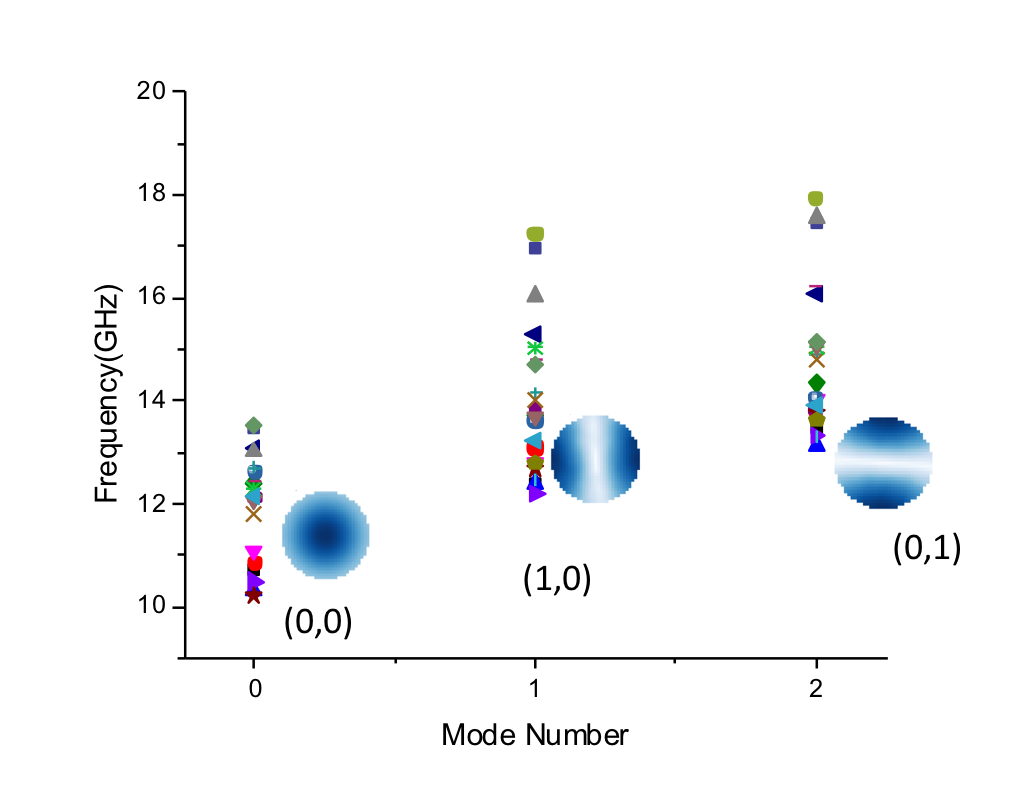
\includegraphics[width=80mm]{fig/broken/stastic-1.png}}
\subfigure{\label{fig:stat2}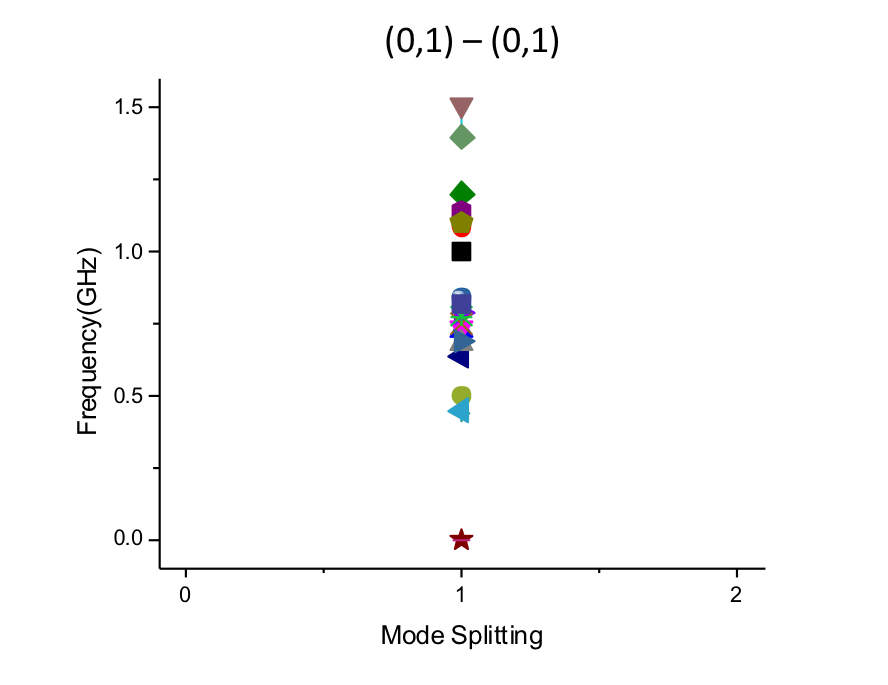
\includegraphics[width=80mm]{fig/broken/stastic-2.png}}
\caption{(a) Statistics of the mode frequencies at zero field for different modes. (b) Statistics of mode splitting between the (1,0) and (0,1) modes for 80 nm samples.
}
\end{figure*}


\begin{figure*}[h!]
\centering     
\subfigure{\label{fig:freq10}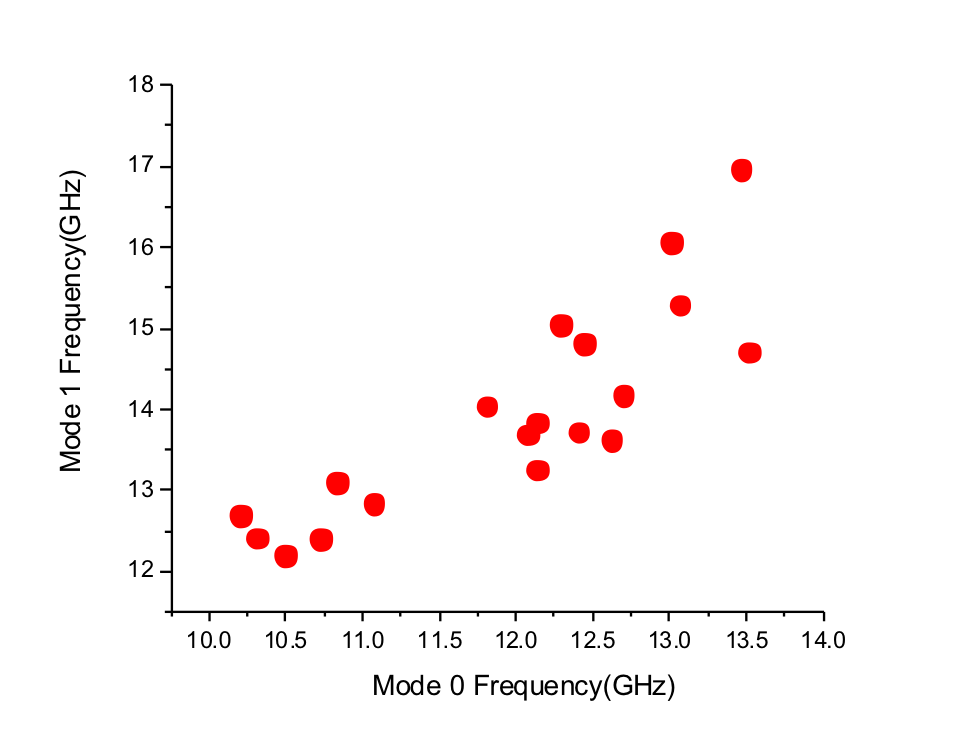
\includegraphics[width=80mm]{fig/broken/freq1-0.png}}
\subfigure{\label{fig:freq20}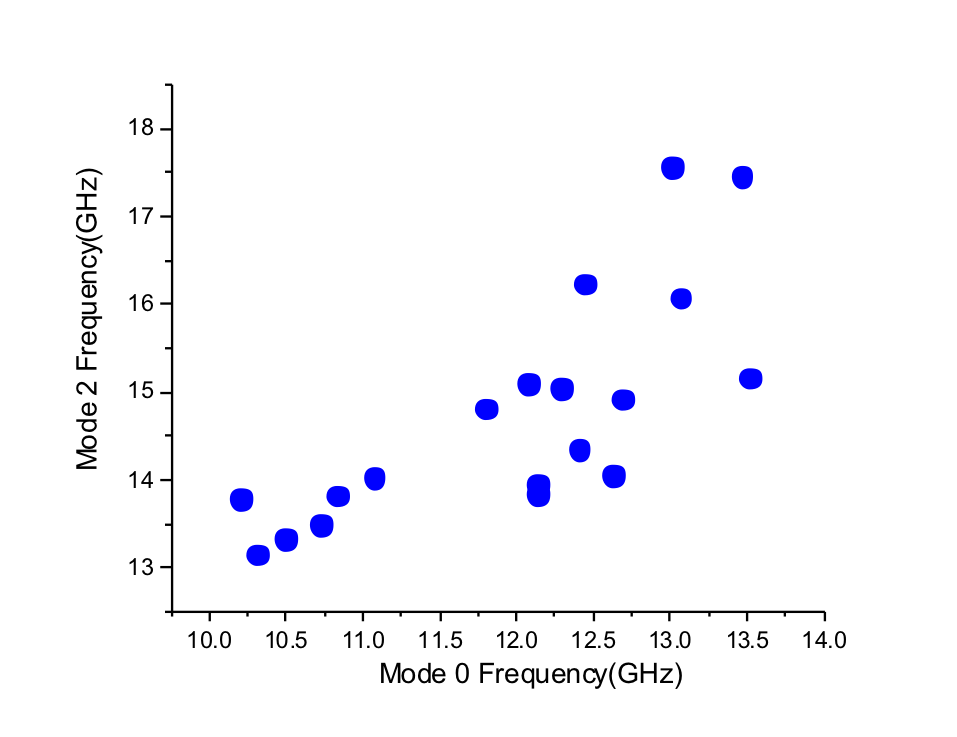
\includegraphics[width=80mm]{fig/broken/freq2-0.png}}
\caption{Statistics of mode splitting for 80 nm sample. (a):Frequency of the Mode 1 versus frequency of the Mode 0. (b):Frequency of the Mode 2 versus frequency of the Mode 0}
\end{figure*}



The (0,0) mode frequencies can be used to quantify the average anisotropy field and the anisotropy field distribution. It is also interesting to compare the distributions of the main modes as a function of the device dimensions. Fig.\ref{fig:freq10} shows the frequency of the Mode 1 versus frequency of the Mode 0 and Fig.\ref{fig:freq20} shows the frequency of the Mode 2 versus frequency of the Mode 0. We can find a clear linear correlation between the quasi-uniform and the higher order mode frequencies, which reveals sample-to-sample perpendicular anisotropy fluctuations but fairly sample-independent exchange energy of the free layer. Since the exchange energy is closely related with sample dimensions, this also shows that the device geometries do not have large variations.


As we mentioned earlier, micromagnetic simulations of circular devices do not match with experimental data. Fig.\ref{fig:exp_spectrum} ST-FMR spectrum of spin wave eignemodes in a circular 60 nm diameter MTJ nanopillar measured at 1 kG out-of-plane field. There are five modes are visible at low frequency and we are concentrating on the lowest three spin-wave modes. Fig.\ref{fig:spectrum_60} shows a simulated spectrum for a 60 nm STT-MRAM element. Vertical dashed lines indicate measured mode positions. Experimentally the frequency spacing between mode 1 and mode 2 is less than 1 GHz. However, the spacing in the micromagnetic simulations is quite large.


\begin{figure*}[h!]
\centering     
\subfigure{\label{fig:exp_spectrum}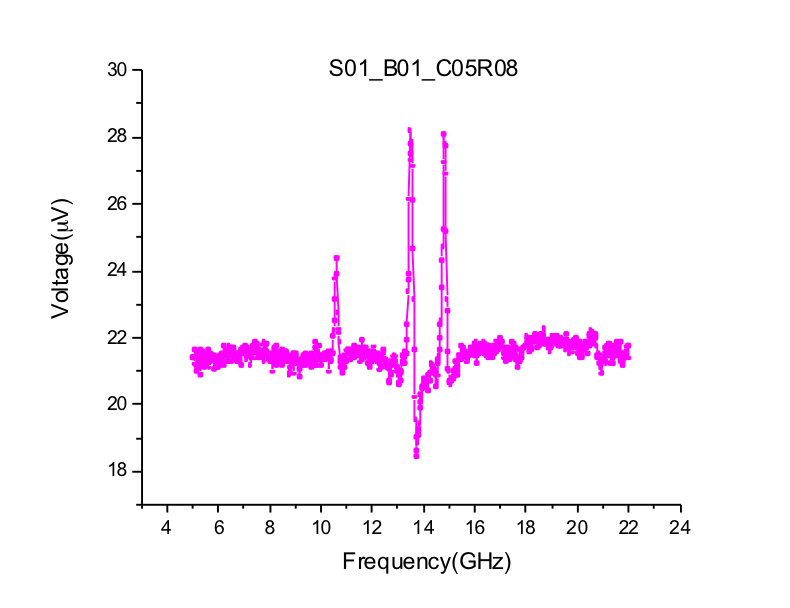
\includegraphics[width=80mm]{fig/broken/exp_spectrum.png}}
\subfigure{\label{fig:spectrum_60}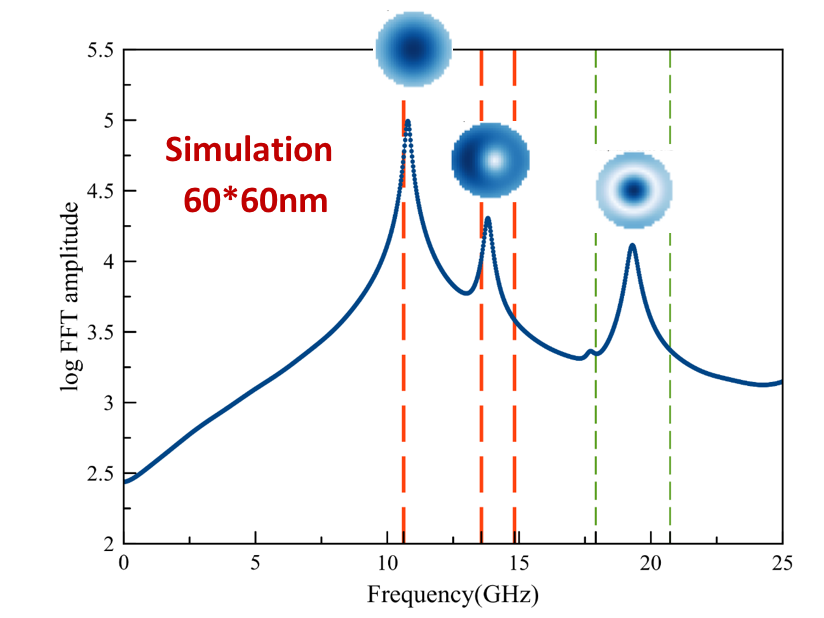
\includegraphics[width=80mm]{fig/broken/spec_60nm.png}}
\caption{(a) ST-FMR spectrum of spin wave eignemodes in a circular 60 nm diameter MTJ nanopillar measured at 1 kG out-of-plane field. (b)Simulated ST-FMR spectrum of a 60 nm circular STT-MRAM element. Vertical dashed lines indicate measured mode positions. Micromagnetic simulated mode profiles are shown next to each mode.}
\end{figure*}


The mode structures and discrepancy can be explained if the perfect circular symmetry of the system is broken. There are several candidates for this broken symmetry and the most possible one is the elliptical distortion of the nanopillar shape. During the fabrication of the STT-MRAM elements, certain processes, such as edge etching, are prone to cause device actual dimension to deviate from perfect circular shape.Such symmetry breaking has little effect on the quasi-uniform (n=0,L=0) mode, but it splits the (n=0,L=1) mode into two modes with a single node along either the short or the long axis of the ellipse. We then examine the effect of the shape distortion on the excited spin wave mode structure via micromagnetic simulations.  In the simulations, we replace the perfect circular shape by an ellipse with varying eccentricity. By varying eccentricity, we influence the degree of the spin wave mode splitting. Fig.\ref{fig:spectrum_68_52} shows a spectrum with device dimension 68 nm * 52 nm. The mode (0,1) split into two modes as we expect. Fig.\ref{fig:spectrum_64_56} shows a spectrum with device dimension 64 nm * 56 nm. As we can compare between those two spectrums, the first-order mode splits into two modes and the frequency gap between those two modes is increasing with increased eccentricity. For devices with larger eccentricity the mode gap is larger, which indicates the mode gap is closely related with shape deviations from perfect circular.

\begin{figure*}[h!]
\centering     
\subfigure{\label{fig:spectrum_64_56}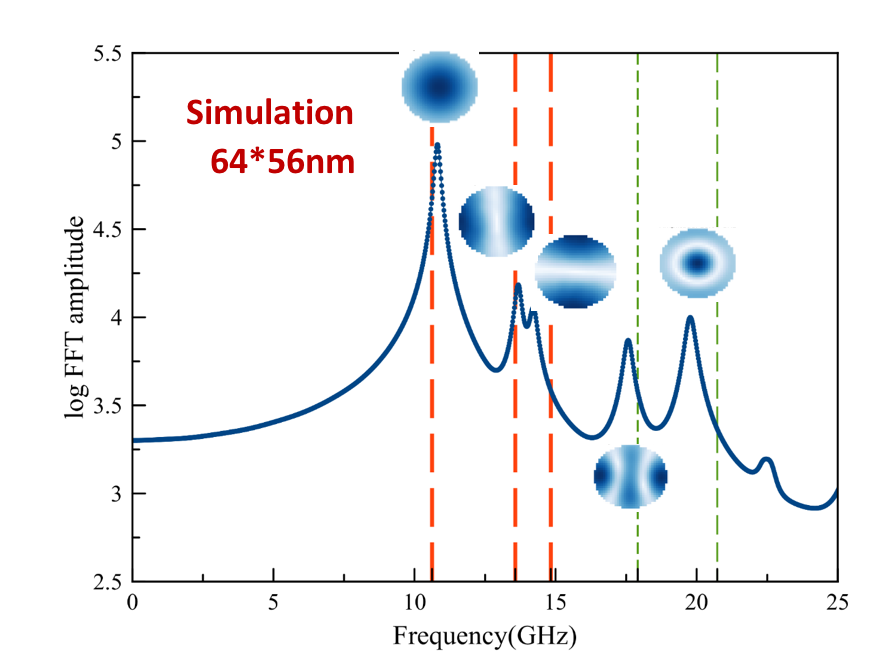
\includegraphics[width=50mm]{fig/broken/spec_64_56nm.png}}
\subfigure{\label{fig:spectrum_68_52}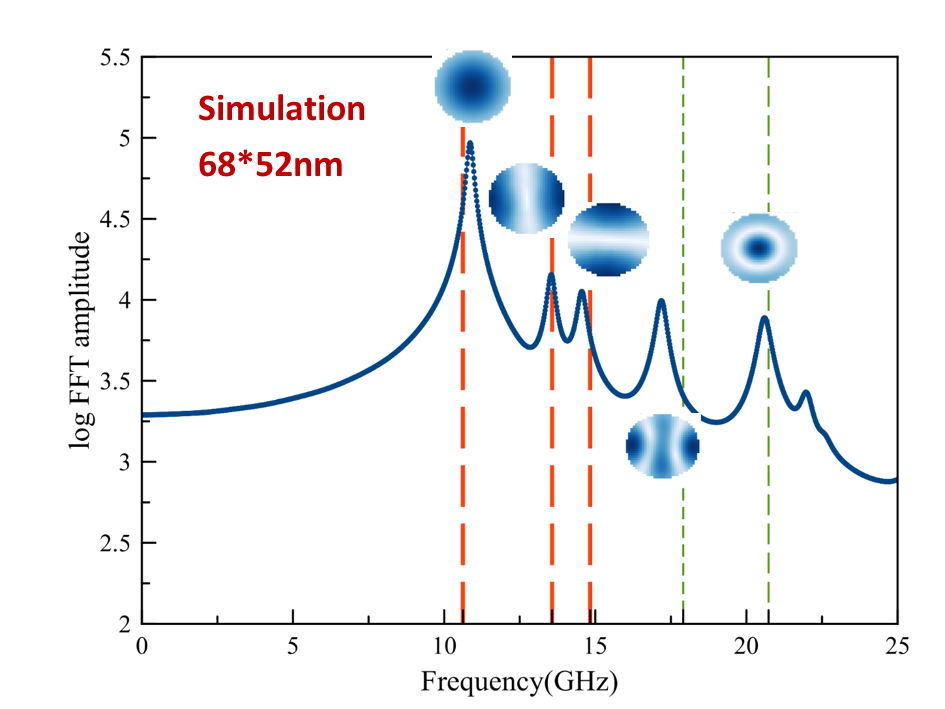
\includegraphics[width=50mm]{fig/broken/spec_68_52nm.png}}
\subfigure{\label{fig:eccentricity}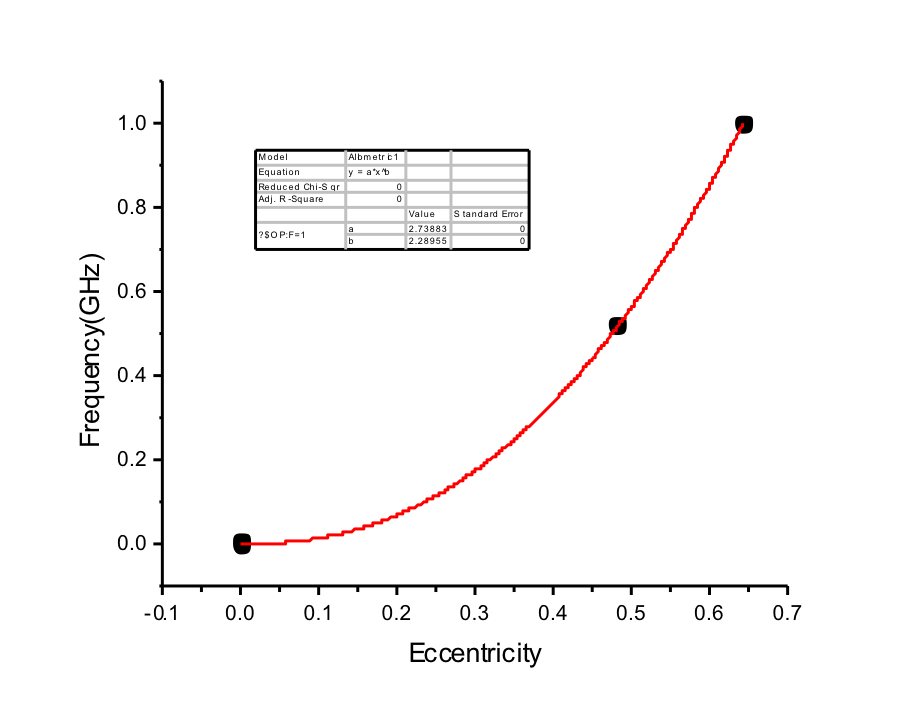
\includegraphics[width=50mm]{fig/broken/ecc.png}}
\caption{ST-FMR spectrum of spin wave eignemodes in a circular 60 nm diameter MTJ nanopillar measured at 1 kG out-of-plane field. Five modes are visible at low frequency. (b)Simulated ST-FMR spectrum of a 5268 nm2 elliptical STT-MRAM element. Vertical dashed lines indicate measured mode positions. Micromagnetic simulated mode profiles are shown next to each mode.  (right) Simulated splitting (frequency gap) of (n=0,L=+1) mode plotted versus eccentricity}
\end{figure*}


With that in mind, Fig.\ref{fig:spectrum_64_56} shows the best micromagnetic fit to the experimental spectrum for a circular 60 nm MTJ nanopillar shown in Fig.\ref{fig:exp_spectrum}. The vertical dashed lines indicate the measured mode frequencies. The simulated mode frequencies agree well with the experimental results suggesting that the mode splitting observed in the experiment arises from MTJ shape distortions. The micromagnetic fitting gives the value of the perpendicular anisotropy (Ku = $4.3*10^5 J/m^3 $) and exchange stiffness constant (A = $6.01*10^{-12}$ J/m) of the free layer.  Furthermore, Fig.\ref{fig:eccentricity} shows simulated splitting (frequency gap) of (n=0,L=+1) mode plotted versus eccentricity. This enables us to establish a correlation between the measured frequency gap and the degree of shape distortion, which is difficult to measure directly.






\begin{figure}[h!]
  \centering
  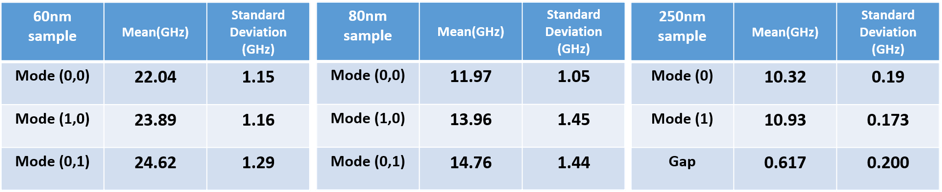
\includegraphics[width=0.8\textwidth]{fig/broken/stastic-mode.png}
   \caption{Three lowest-frequency spin wave eigenmodes of the free layer of a circular STT-MRAM sample with 60 nm diameter. The top image shows the spatial map of the amplitude of the mode while the bottom image shows the spatial map of the spin wave mode’s phase}
  \label{fig:statmod1}
\end{figure}


We then study the mode splitting as a function of the nanopillar diameter. More than 15 devices of each MTJ diameter were measured to obtain reliable statistical distributions of the mode frequencies.  First, we find that the 250 nm devices do not show splitting of the (n=0,L=+1) mode. This supports the picture of splitting of this mode due to deviations from the perfectly circular shape (little process-induced ellipticity is expected for these large circular devices). Second, for the larger 250 nm devices, standard deviation of the frequency distribution is much smaller than that for the 60 nm and 80 nm devices. We can then conclude that low-energy mode frequencies are sensitive to the average anisotropy over the free layer area. In the larger devices, averaging over a larger number of crystallographic grains and results in a tighter distribution of the free layer anisotropy values.







\newpage

\section{Possible Origin of WER Correlation with ST-FMR}

We also collected preliminary data suggesting a correlation between ST-FMR spectra of circular MTJ nanopillars with write error rates of the devices.  Fig.\ref{fig:WERSTFMR} shows ST-FMR spectrum of spin wave eignemodes in a circular 40 nm diameter MTJ nanopillar as a function of out-of-plane magnetic field. This sample shows anomalous WER behavior (ballooning).

\begin{figure}[h!]
  \centering
  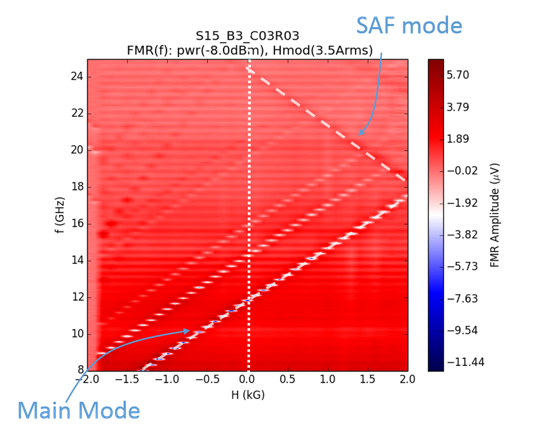
\includegraphics[width=0.6\textwidth]{fig/FieldMod/FMR-WER.png}
   \caption{ST-FMR spectrum of spin wave eignemodes in a circular 40 nm diameter MTJ nanopillar with known anomalous WER behavior measured as a function of out-of-plane magnetic field. The SAF spin wave mode and the quasi-uniform free layer mode are labeled by dashed lines in the figure.}
  \label{fig:WERSTFMR}
\end{figure}


For this device, the frequency of the SAF mode in zero field is nearly twice the resonance frequency of the quasi-uniform mode of the free layer. This frequency coincidence condition suggests that a nonlinear three-magnon process (confluence of two magnons of the quasi-uniform mode into a single SAF mode magnon) should be resonant for this device in zero field. Such non-linear resonant scattering channel can drain energy an angular momentum supplied by spin torque t the free layer and impede the free layer switching process. Therefore, this nonlinear scattering process is suspected origin of the anomalous WER behavior. For all devices studied so far, we find that MTJs exhibiting anomalous WER do satisfy this nonlinear resonant scattering (frequency coincidence) condition, while all devices with normal WER do not satisfy the nonlinear resonant scattering condition.




\section{Field Modulated Mag-noise Measurement}



We have developed a novel method of experimental characterization of the spectrum of spin wave eigenmodes of individual STT-MRAM elements. This method is magnetic noise spectroscopy with magnetic field modulation. Previous work\cite{MagnoisePRL}\cite{Magnoise} has demonstrated that even by applying a small DC current which is considerably smaller than the critical switching current, there will be a significant influence of spin transfer torque on thermally activated ferromagnetic resonance excitations. However it has not been showed that the Magnoise measurement can be applied to the Magnetic Tunnel Junctions(MTJs) with perpendicular magnetic anisotropy(PMA). We are also interested in applying the field modulation technique as we did from the ST-FMR measurement.


Fig.\ref{fig:magnoise-setup} shows the experimental setup for measuring magnetic noise with magnetic field modulation, in which a microwave-frequency noise emitted by the STT-MRAM at a finite bias current is measured via a lock-in detection

\begin{figure}[!ht]
  \centering
  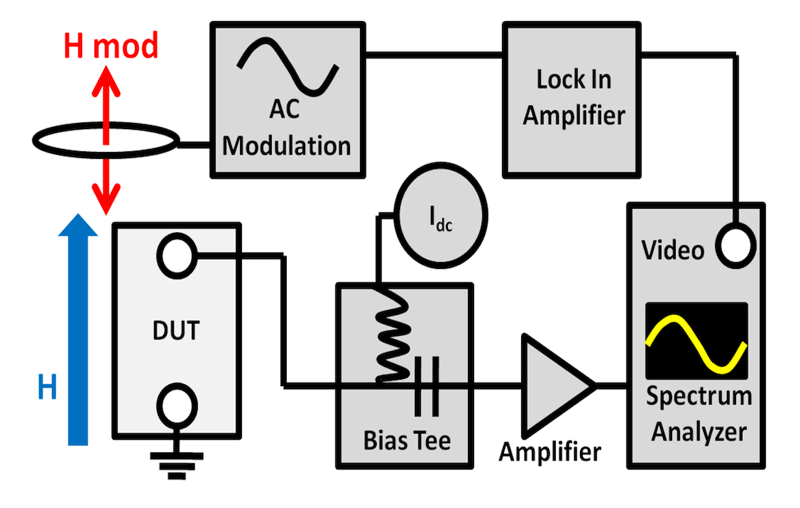
\includegraphics[width=0.6\textwidth]{fig/magnoise/Picture1.png}
   \caption{Set-up for Magnoise measurement}
  \label{fig:magnoise-setup}
\end{figure}

technique. The microwave noise is emitted at the frequencies of spin wave eigenmodes of the sample, with the most prominent features arising from spin wave eigenmodes of the free layer. The different between the Magnoise measurement and the ST-FMR measurement is that, other than using a microwave generator to send a ac current into the MTJs, the MTJs are excited by a DC current and the spectrum analyzer is used to detect the ac signal at the resonance frequency.

\begin{figure}[!ht]
  \centering
  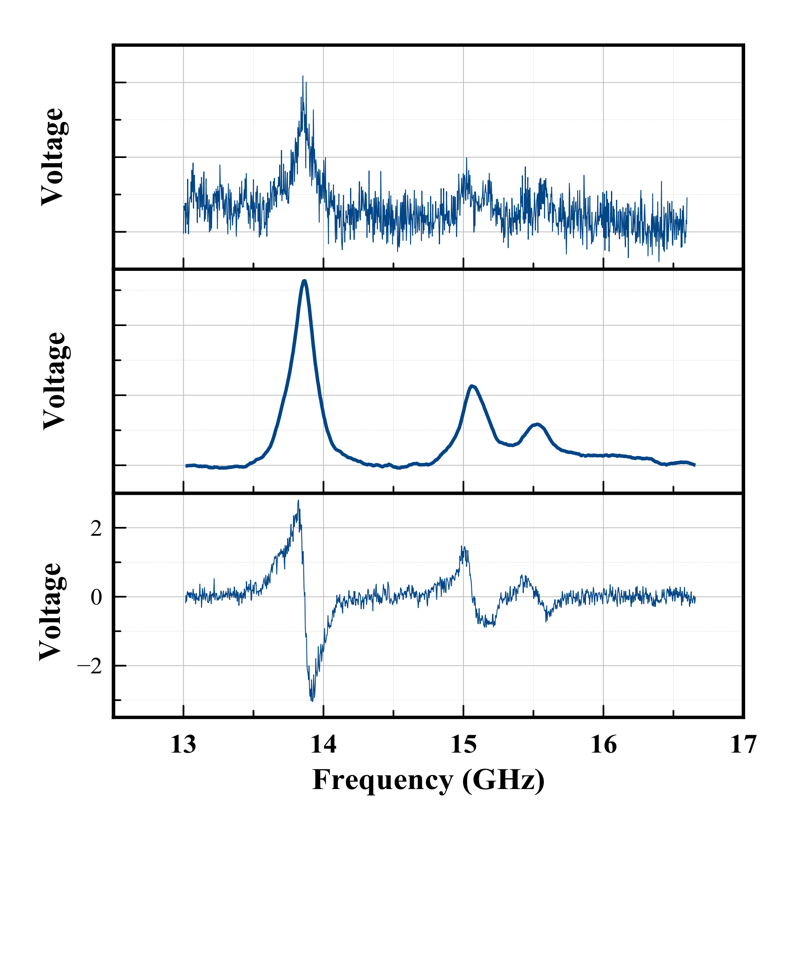
\includegraphics[width=0.6\textwidth]{fig/magnoise/magnoise-data.png}
   \caption{Summary of the magnoise measurement. Top: Raw spectrum taken without the field modulation. Middle: Integration of the spectrum taken with the field modulation. Bottom: Raw spectrum taken with the field modulation technique.}
  \label{fig:magnoisedata}
\end{figure}


The top panel of Fig.\ref{fig:magnoisedata} shows the magnetic noise spectrum measured by conventional technique without magnetic field modulation. The conventional method only allows us to reliably measure the frequency of the quasi-uniform spin wave mode. The linewidth of the main mode is hard to fit accurately. We can also only measure the main mode and do not have enough resolution to accurately fit for the higher order modes. In contrast, the data obtained with magnetic field modulation shown below allow us to detect not only the resonant frequencies but also the spectral linewidth of several spin wave modes of the device. This is enabled by the superior signal-to-noise factor of our technique with magnetic field modulation. The bottom panel of Fig.\ref{fig:magnoisedata} shows the same spectrum taken with field modulation technique. The signal-to-noise ratio is much improved and the higher-order modes can be resolved. To illustrate the nature of our field-modulation technique, in the middle panel of the Fig.\ref{fig:magnoisedata} we plot the integration of the bottom spectrum from the Fig.\ref{fig:magnoisedata}. The integrated spectrum resembles the raw spectrum taken without field-modulation technique with all the excited modes coincide with each other. We can conclude that the field-modulation technique only improves the signal-to-noise ratio without distorting the spectrum. The data obtained with magnetic field modulation is of high enough quality to enable determination of the Gilbert damping, magnetic anisotropy and exchange stiffness constant of the free layer. 


Now we would like to benchmark between the magnoise noise method and ST-FMR on a typical STT-MRAM cell. Fig.\ref{fig:noiseMR} shows the magnetoresistive curve of the MTJ sample explored in this study. This device has TMR ratio around 180 percent and the coercive field close to 2 kG. Fig.\ref{fig:noiseFMR2D} shows the ST-FMR spectrum of this device at the AP state with three spin-wave modes excited. 

\begin{figure}[!ht]
\centering
\subfigure{\label{fig:noiseMR}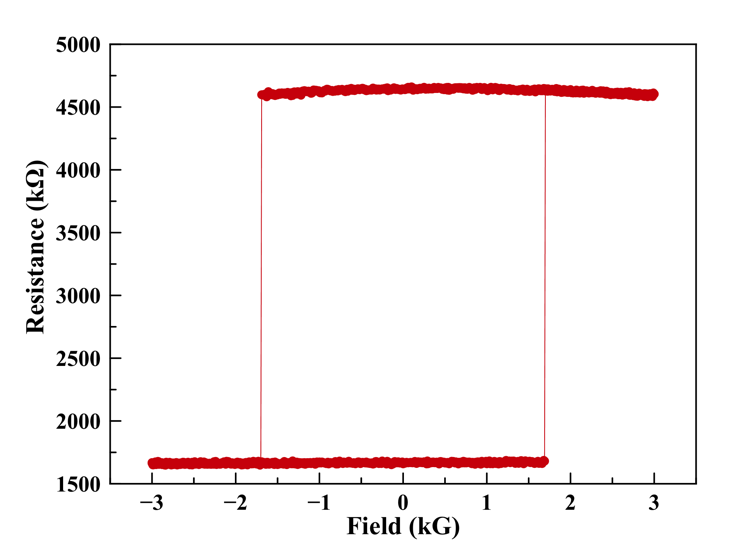
\includegraphics[width=75mm]{fig/magnoise/noiseMR}}
\subfigure{\label{fig:noiseFMR2D}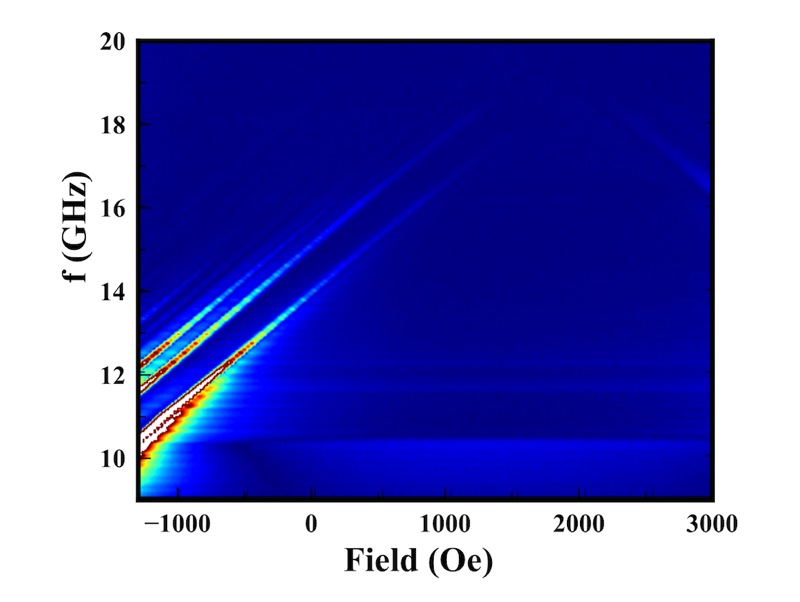
\includegraphics[width=75mm]{fig/magnoise/noiseFMR2D}}
\caption{(a) The magnetoresistive curve of the studied sample with the TMR ratio around 180 \% and the coercive field close to 2 kG. (b) measured ST-FMR 2D spectrum of this device. Three spin-wave modes are visible.}
\end{figure}

One major feature of the magnoise measurement is to allow large dc bias into the MTJ and study the bias-dependent shift of resonance field and linewidth. Fig.\ref{fig:magnoise-2D} shows dc-dependent spectrum taken from the magnoise measurement. Fig.\ref{fig:magnoise-2D}(a) shows the direct measurement of the bias-dependent magnoise measurement. Fig.\ref{fig:magnoise-2D}(b) shows the integration of the raw spectrum under dc-bias. Three spin wave modes are visible as labelled. 

\begin{figure}[!ht]
  \centering
  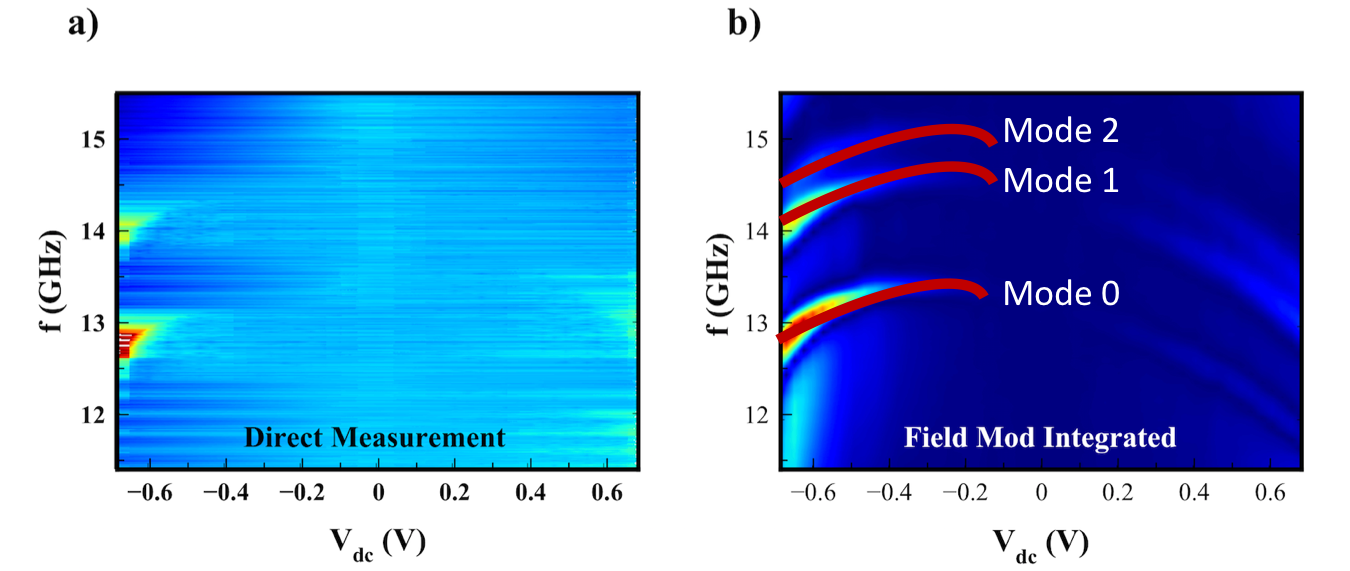
\includegraphics[width=1.0\textwidth]{fig/magnoise/magnoise2D.png}
   \caption{(a) Direct measurement of the bias-dependent magnoise measurement. (b) Integration of the raw spectrum under dc-bias. Three spin wave modes are visible as labelled. }
  \label{fig:magnoise-2D}
\end{figure}

Now we can directly compare the bias-dependent measurement and main mode fitting using these two techniques. Fig.\ref{fig:FMRfreq} shows the frequency-domain ST-FMR measurement and Fig.\ref{fig:Noisefreq} shows the frequency-domain magnoise measurement. We fit both the resonance frequency on the top panel and the linewidth on the bottom panel. When at the AP state, negative dc bias is the anti-damping spin-torque and can switch the MTJ from the AP state to the P state. There are several observations from the comparisons. First of all, ST-FMR can still measure the data with small(even zero) dc bias while the magnoise measurement is not feasible without large dc bias.

\begin{figure}[!ht]
\centering
\subfigure{\label{fig:FMRfreq}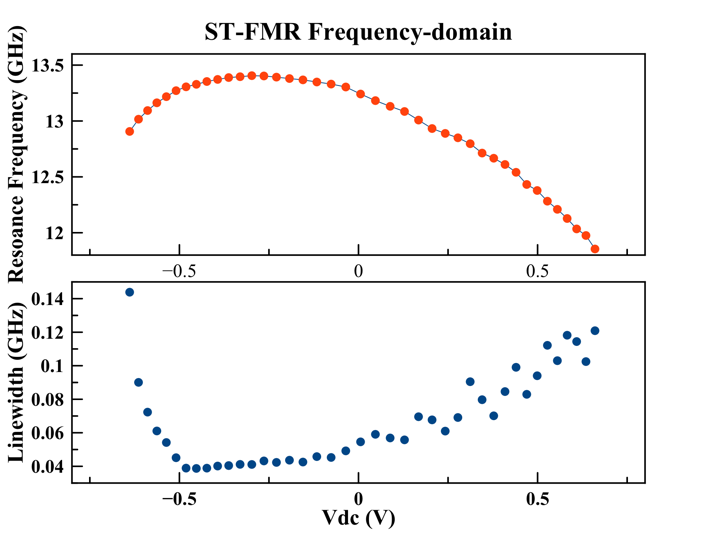
\includegraphics[width=75mm]{fig/magnoise/STFMR-freq.png}}
\subfigure{\label{fig:Noisefreq}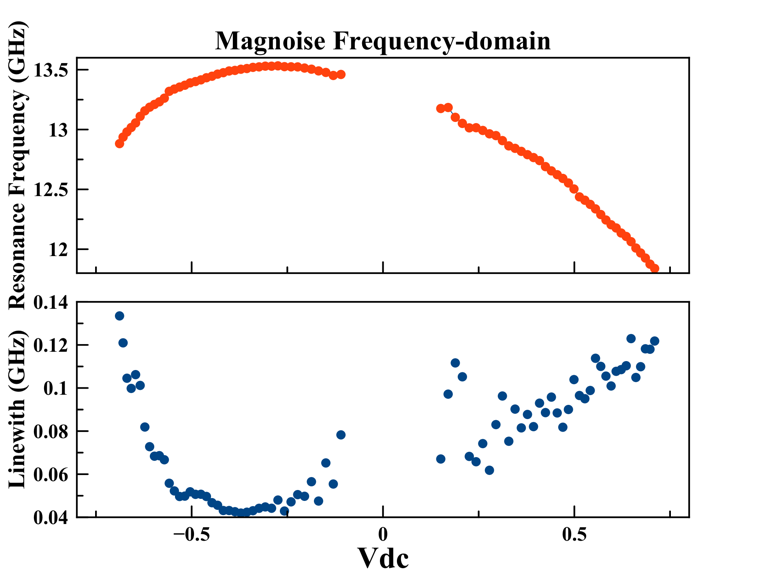
\includegraphics[width=75mm]{fig/magnoise/noise-freq}}
\caption{(a) ST-FMR data on the frequency domain as a function of dc bias voltage (b) Magnoise data on the frequency domain as a function of dc bias voltage}
\end{figure}

Secondly, the quantitate value between those two measurements are quite close to each other. This is a important sanity check since the measurement resonance frequency and linewidth should only be determined by intrinsic material properties of the MTJ we studied, not by the experimental methods utilized. For example, the linewidth in both measurement goes to large value when approaching bigger negative dc bias(close to MTJ switching).


\begin{figure}[!ht]
\centering
\subfigure{\label{fig:FMRfield}\includegraphics[width=75mm]{fig/magnoise/FMR-field}}
\subfigure{\label{fig:Noisefield}\includegraphics[width=75mm]{fig/magnoise/noise-field}}
\caption{(a) ST-FMR data on the field domain as a function of dc bias voltage (b) Magnoise data on the field domain as a function of dc bias voltage}
\end{figure}


Thirdly, we find that the ST-FMR measurement has better signal-to-noise ratio. It is better expressed in the linewidth measurement under larger positive dc bias where the ST-FMR data has less fluctuations. To better compare the ST-FMR and the magnoise measurement, we also make field-domain dc-bias using these two methods. Fig.\ref{fig:FMRfield} shows the field-domain data from the ST-FMR and Fig.\ref{fig:Noisefield} shows the field-domain data from the magnoise noise measurement. The linewidth data shows a considerably larger fluctuations from the magnoise noise measurement at the positive bias current while the ST-FMR still shows a good linear relation.

In summary, the main feature of the magnetic noise method is that it allows measurement of the spin wave spectrum faster than the ST-FMR method.  Therefore, this method can be used for rapid screening of magneto-dynamic properties of STT-MRAM cells. However, by compared with the ST-FMR methods in both frequency-domain and field-domain, we find that the ST-FMR usually yields better signal-to-noise ratio spectrum.



\clearpage

\section{In-plane ST-FMR measurement and Mode identification}

While the Spin-torque Ferromagnetic Resonance(ST-FMR) technique is a powerful tool of detecting the spin-wave eigenmodes within the free layer of the Magnetic Tunnel Junctions(MTJs), one needs to be careful about the "modes" excited in the experimental spectrum. There are two main concerns here. First of all, it is important to excite all the spin wave modes of the free layer, from the lowest-frequency quasi-uniform mode to higher modes. Due to different excitation mechanism, either the quasi-uniform mode or some of the higher order modes are possible to be weak in the ST-FMR signal. Mislabelling the modes makes further analysis impossible. 
 Furthermore, as we have seen from the previous chapter, exchange coupling between the free layer and the SAF layer, if not dominant, does exist within the MTJs. Most of the time, we are mainly interested in the free layer dynamic properties and we do not wish to have SAF layer modes mixed with the free layer modes. These two problems are better explained in the following example.

\begin{figure}[!ht]
\centering
\subfigure{\label{fig:S6AP}\includegraphics[width=75mm]{fig/in-plane/S6-B3-R6-C13-AP-STATE}}
\subfigure{\label{fig:S6P}\includegraphics[width=75mm]{fig/in-plane/S6-B3-R6-C13-P-STATE}}
\caption{2D contour plot of ST-FMR spectrum taken at AP state(left) and P state(right). Both AP and P state has four lowest obvious spin-wave modes but with different mode spacings.}
\end{figure}

When we have a big MTJ device and the density of spin-wave modes is large due to later confinement, it is more difficult to identify all the modes excited in the spectrum. Fig.\ref{fig:S6AP} shows a ST-FMR 2D contour plot of a $120*60  nm^2$ device. At least we can identify four obvious spin-wave modes from this spectrum with lowest two modes very close to each other. If we focus on one constant-field vertical line, we can see the first mode and the second mode are very close to each other while the amplitude of the first mode is much smaller than the second one. If we look at the 2D ST-FMR contour plot at the parallel state shown in the Fig.\ref{fig:S6P}, it would not make the spin-wave modes identification easier. At the parallel state we also have identified four spin-wave modes with a decent larger gap between the first mode and the second. However we know that the mode spacings are determined by the exchange stiffness of the free layer and there should not be such a obvious difference between the AP and P state. There are generally(which is not necessarily present in the current case) two problems when measuring the MTJ at the parallel state. First of all, the ST-FMR signal is proportional to the absolute value of resistance oscillations under the ac current drive, which is less dominant in the parallel state. This means the parallel state has less signal amplitude compared with the AP state, especially for the quasi-uniform mode. Another problem is that, at the parallel state, since the SAF top layer is parallel to the free layer, it might be possible to excite the SAF modes close to the free layer mode.


\begin{figure}[!ht]
\centering
\subfigure{\label{fig:S6APDC}\includegraphics[width=75mm]{fig/in-plane/ap-dc}}
\subfigure{\label{fig:S6PDC}\includegraphics[width=75mm]{fig/in-plane/p-dc}}
\caption{Bias dependent ST-FMR spectrum taken at the constant driven frequency 16 GHz for both AP state(left) and P state(right). All the spin-wave modes have the same curvature versus bias.}
\end{figure}

The first type of measurements we can make to ensure we excite the free layer spin-wave modes only is to perform DC bias-dependent ST-FMR for both AP and P state. Because of the different spin torque polarity, the free layer and the SAF layer modes should have different curvature when applying the non-zero finite bias current. As we discussed in the previous section, the study of the linewidth as a function of dc bias can also be utilized to fit for the critical voltage of the MTJs. In Fig.\ref{fig:S6APDC} and Fig.\ref{fig:S6PDC} we have the bias dependent ST-FMR scan at the fix frequency 16 GHz for both AP and P state. What we find is that all the modes we observed at the previous ST-FMR 2D field dispersion contour plot have shown the same curvature under finite bias. This curvature is often determined by the combination of the voltage-controlled magnetic anisotropy and ohmic heating effect.


\begin{figure}[!ht]
\centering
\subfigure{\label{fig:S6APOUT}\includegraphics[width=75mm]{fig/in-plane/S6-B3-R6-C13-AP-STATE}}
\subfigure{\label{fig:S6APIN}\includegraphics[width=75mm]{fig/in-plane/S6-B3-R6-C13-inplane}}
\caption{2D contour plot of ST-FMR spectrum taken at AP state with out-of-plane field applied(left) and in-plane field(right). Both spectrum has four lowest spin-wave modes with different relative amplitude.}
\end{figure}

So far we can conclude that all the spin-wave modes we saw in the out-of-plane ST-FMR measurements are from the free layer. Now we need to identify all the modes without missing some of the modes. We then perform ST-FMR measurement applying the in-plane magnetic field. When we apply the in-plane magnetic field to this MTJ with perpendicular magnetic anisotropy, we will create misalignment between the free layer and the fixed layer by introducing the hard axis magnetic field. From the Fig.\ref{fig:S6APIN} we see such a 2D spectrum with in-plane magnetic field applied at the AP state. In this measurement, the quasi-uniform mode has the largest amplitude compared with other modes due to introduced misalignment. It is also clear that the amplitude of the quasi-uniform mode decrease as the magnetic field decrease. When approaching zero magnetic field, the uniform mode almost becomes invisible. This also help us understand why under perpendicular magnetic field, the main mode is hard to excite. In the next step, we can fit for the modes we excited in the in-plane spectrum and compare with the out-of-plane data. Here for better comparison, we also show the out-of-plane spectrum for the AP state in the Fig.\ref{fig:S6APOUT}. From both the spectrum we can at lease identify four spin-wave modes and we can fit four of them at zero magnetic field(out-of-plane or in-plane). 


\begin{table}[h!]
\centering
\begin{tabular}{||c c c||} 
 \hline
 Experiment & Out-of-Plane & In-Plane\\ [0.5ex] 
 \hline\hline
 Mode 0 (GHz) & 15.63 & 15.42\\ 
 \hline
 Mode 1 (GHz) & 16.33 & 16.23\\
 \hline
 Mode 2 (GHz) & 18.28 & 18.28\\
 \hline
 Mode 3 (GHz) & 19.22 & 19.12 \\ [1ex] 
 \hline
\end{tabular}
\caption{Comparisons between four lowest spin-wave modes at AP state at zero magnetic field with different magnetic field direction(easy-axis out-of-plane and hard-axis in-plane) applied.}
\label{table:APtoP}
\end{table}

The table \ref{table:APtoP} summarizes the mode fitting results. Within certain deviations, it can be seen from the above results that we have good agreements between out-of-plane and in-plane measurements. Moreover, since in-plane hard-axis measurements are able to excite all the spin-wave modes, we can now be confident about our out-of-plane measurement without missing the free layer modes.

%\chapter{Time-domain measurement of spin-torque switching in MTJs}

As we have discussed in the previous chapter, magnetization switchin induced by spin-tranfer torque is both useful for understanding the fundamental physics of magnetic dynamics and for applications in magnetic random access memory(MRAM). Measurements in the time domain can provide the most direct information about the switching process. However, the majority of previous time-resolved studies of spin-torque switching required averaging over many events, which would hide individual switching variations. Here we report a single-shot time resolved time-domain measurement similar to the technique developed by Cui.et.al \cite{Cui}. We have shown that the sensitivity of single-shot resistant measurements have been greatly improved and both prior to switching and during spin-torque switching have been resolved. 

\section{Experimental Setup}
Previously, the sketch of time-domain measurement is shown\ref{fig:time_set}. The general idea is the following: by send the pulse into the magnetic tunnel junctions, the transmitted the signal will depend on the resistance of the device. 

\begin{figure}[h]
  \centering
  \includegraphics[width=0.6\textwidth]{fig/time_set.png}
  \caption{Original time-domain setup}
  \label{fig:time_set}
\end{figure}

If there is magnetic state switching happening during the duration of this pulse, we could be able to resolve it by recording the time-domain signal using a Time scope. This method is very straightforward, however, it is not practical in most cases. To illustrate that, let us calculate the transmitted signal.
 If we apply the voltage pulse$V_{inc}$, the transmitted signal will be given as

\begin{equation}
\label{orgi}
V(t) = \frac{V_{inc}}{1+G_S(t)Z_0/2}
\end{equation}
where $G_S(t) = 1/ R_S(T)$ is the sample conductance(the reciprocal resistance), $Z_0=50 \Omega$ is the probe impedance. Typically the resistance of the devices is around several thousands ohms, so we have a very strong impedance mismatching here. We can expand the time-dependent voltage signal with respect to a reference, if we use the parallel state conductance $G_P$ as the reference value, and write $G_S(t)$ as $G_S(t) = G_P + \Delta G(t)$, since $\Delta G(t) Z_0$ is usually much less than 1, we can expand Equation \ref{orgi} as the following:
\begin{equation}
\label{deltaequ}
V(t) = \frac{1}{1+G_PZ_0/2}V_{inc} + \frac{Z_0/2}{(1+G_PZ_0/2)^2}V_{inc} \Delta G(t)
\end{equation}

The first term in Equation\ref{deltaequ} is related to the resistance mismatch between the device and RF probe. The second term is coming from the resistance change associated with magnetic dynamics. If we would like to monitor the device resistance, we should expect the second term to be large, at least well above the noise level. However, as we point out, because of the impedance mismatching, the second term would be really smaller, usually around several mill volts. This requires lots of averaging to improve the signal to noise ratio and thereby hide each single switching event.

To improve our signal to noise ratio, we adapt improved measurement set-up shown in Fig.\ref{fig:time_domain}. As usual, we apply the pulse from a pulse generator. This time, however, we split the into two identical copies. The first copy goes into the device and induce magnetic switching. The second pulse will go through a pulse inverter and it will flip the polarity. What is important here is to choose the pulse inverter so that it does not distort the waveform too much. After the first copy goes through the device, we use a power combiner to combine these two pulses in a way that these two copies should enter the power combiner at the same time. 

\begin{figure}[h]
  \centering
  \includegraphics[width=0.8\textwidth]{fig/time_domain}
  \caption{Improve time-domain set-up}
  \label{fig:time_domain}
\end{figure}

To accomplish that, we would like to carefully tune the time delay of there two lines so that they have been correctly synchronized. In the current set-up, we adjust the time delay by varying the microwave cable length in the circuit. After we combine these two pulses, we use an amplifier to amplify the signal and send it into the storage scope. In this process, the signal left after we combine these two pulses would only be the part depending on the magnetic state, where any other type of noise should be canceled out. This should greatly improve the signal-to-noise ratio.

Before we go to the experiment discussion, we would like to discuss another important source of noises in these type of experiments. Ideally, we want to amplify our voltage signal after the power combiner to be large enough. However, we also have to fight with the bit noise induced by the storage scope. We are using a 64-bit time scope, the bit noise in the measurement is proportional to the voltage resolution used in the time scope. So in order to reduce the bit noise, smaller voltage resolution should be adapted and the signal has to be small enough to fit in this small voltage resolution. Practically, after we amplify the voltage signal, we use proper attenuator(usually around -10 dB).

\section{Results and Discussion}

Now we have set-up correct time delay and pick appropriate attenuation in the circuit, we can send the pulse and observe the time dependent signal. Fig.\ref{fig:Total_sig} shows a typical signal we resolve from a switching. We first initialize the MTJ into anti-parallel state and send through a positive pulse. The polarity of positive pulse corresponds to damping for the anti-parallel state, so this positive pulse should not induce magnetic switching for anti-parallel state. We record the anti-parallel state signal as the background and label it as AP in Fig.\ref{fig:Total_sig}. 

\begin{figure}[h]
  \centering
  \includegraphics[width=0.8\textwidth]{fig/total_sig}
  \caption{A switching signal from time-domain measurement. Anti-parallel signal(blue), PtoAP signal(red) along with the voltage difference(Green)}
  \label{fig:Total_sig}
\end{figure}


Then, we initialize the MTJ into parallel state and re-send the positive voltage(which is anti-damping for parallel state). Then we record this signal from the time scope and label as P to AP in Fig.\ref{fig:APtoP}. One can clearly find that at the beginning of the pulse, AP and PtoAP signal are clearly separated. At the middle of the pulse, the PtoAP pulse suddenly shifts into AP signal, which is related to the magnetic state change in the MTJ. So we have observe a magnetic switching in time-domain. We can also subtract the background AP signal from the PtoAP and plot it labeled as Difference in Fig.\ref{fig:diff}. If we look at the Difference signal, we can see that at the beginning of the pulse, the difference is around 30 mV, then it drops to - 10 mV. So we can well separate the anti-parallel and parallel state.

\begin{figure}[!ht]
\centering
\subfigure{\label{fig:APtoP}\includegraphics[width=80mm]{fig/APtoP.png}}
\subfigure{\label{fig:diff}\includegraphics[width=80mm]{fig/diff.png}}
\caption{(a) Zoomed PtoAP signal(red) and AP state background(blue) (b)Zoomed voltage signal difference.}
\end{figure}

Now that we have greatly improved the voltage signal to separate two magnetic states, we can study individual switching event without perform averaging to reduce the noise. One thing we can study is the distribution of switching time. From Fig.\ref{fig:26} to Fig.\ref{fig:9} we show several traces from different switching events. Here we only demonstrate the different signals between two state. One can clear find that for different switching traces, we have different switching time, ranging from 2.6 ns, which is at the beginning of the pulse, to 9 ns, which is at the very end of the pulse. This indicates the random nature of this single shot-switching. More importantly, we can obtain a good statistics of switching time as a function of input parameters. Also we find that in Fig.\ref{fig:no} we find that at a fixed voltage, we can still have non-successful switching event, where we find that for this non-successful switching attempt, the system enters a large oscillation. This enables us to further study the different between successful and non-successful switching events. 




\begin{figure}[!ht]
\centering
\subfigure{\label{fig:26}\includegraphics[width=80mm]{fig/2_6.png}}
\subfigure{\label{fig:67}\includegraphics[width=80mm]{fig/6_7.png}}
\subfigure{\label{fig:9}\includegraphics[width=80mm]{fig/9.png}}
\subfigure{\label{fig:no}\includegraphics[width=80mm]{fig/no.png}}
\caption{Switching events for different individual events.(a)(b)(c) show switching events which switch at 2.6 ns, 6.7 ns and 9 ns respectively. (d) shows the non-switching event. }
\end{figure}

To further illustrate the random nature of magnetic switching in time-domain, we fix the applied voltage at 425 mV and study the distribution of the switching time as it is shown in Fig.\ref{fig:dist}. From other switching probability measurement, we already know that at 425 mV voltage, the device has a very switching probability. From this distribution we find that the switching time is unevenly distributed, it is centered around 4 ns and has a negative skewness. The distribution also gives a very small tail at high switching time, which means switching rarely happens at the tail of the pulse. We try to fit the switching count as a Gaussian function, which gives a good fitting result as it is shown in Fig.\ref{fig:dist}.



\begin{figure}[h]
  \centering
  \includegraphics[width=0.8\textwidth]{fig/dist.png}
  \caption{Distribution of switching time at constant voltage 425 mV.}
  \label{fig:dist}
\end{figure}

If we vary the applied voltage and also measure the switching time distribution as Fig.\ref{fig:dist}, we typically find that the the peak of the distribution and also the skewness are dependent on the applied voltage. For smaller applied voltage, the center of the switching time moves to higher time period and the skewness of the distribution becomes smaller. That indicates that for larger voltage we have more deterministic and fast switching. When the applied voltage is small and the switching probability is low, the switching behavior shows more randomness.








\chapter{Best Things about MTJs}


\section{Critical Voltage Measurement}




\section{Field Modulated Mag-noise Measurement}



The UCI group developed a novel method of experimental characterization of the spectrum of spin wave eigenmodes of individual STT-MRAM elements. This method is magnetic noise spectroscopy with magnetic field modulation. Figure 3(a) shows the experimental setup for measuring magnetic noise with magnetic field modulation, in which a microwave-frequency noise emitted by the STT-MRAM at a finite bias current is measured via a lock-in detection

\begin{figure}[!ht]
  \centering
  \includegraphics[width=0.6\textwidth]{fig/magnoise/Picture1.png}
   \caption{Set-up for Magnoise measurement}
  \label{fig:magnoise-setup}
\end{figure}

technique. The microwave noise is emitted at the frequencies of spin wave eigenmodes of the sample, with the most prominent features arising from spin wave eigenmodes of the free layer. The top panel of Figure 3(b) shows the magnetic noise spectrum measured by conventional technique without magnetic field modulation. The conventional method only allows us to reliably measure the frequency of the quasi-uniform spin wave mode. 






In contrast, the data obtained with magnetic field modulation shown below allow us to detect not only the resonant frequencies but also the spectral linewidth of several spin wave modes of the device. This is enabled by the superior signal-to-noise factor of our technique with magnetic field modulation. The data obtained with magnetic field modulation is of high enough quality to enable determination of the Gilbert damping, magnetic anisotropy and exchange stiffness constant of the free layer. The main feature of the magnetic noise method is that it allows measurement of the spin wave spectrum faster than the ST-FMR method.  Therefore, this method can be used for rapid screening of magneto-dynamic properties of STT-MRAM cells.




\begin{figure}[!ht]
  \centering
  \includegraphics[width=0.6\textwidth]{fig/magnoise/magnoise-data.png}
   \caption{Set-up for Magnoise measurement}
  \label{fig:magnoisedata}
\end{figure}


\begin{figure}[!ht]
\centering
\subfigure{\label{fig:noiseMR}\includegraphics[width=75mm]{fig/magnoise/noiseMR}}
\subfigure{\label{fig:noiseFMR2D}\includegraphics[width=75mm]{fig/magnoise/noiseFMR2D}}
\caption{(a) AP state simulation (b)P state simulations}
\end{figure}



\begin{figure}[!ht]
  \centering
  \includegraphics[width=1.0\textwidth]{fig/magnoise/magnoise2D.png}
   \caption{Set-up for Magnoise measurement}
  \label{fig:magnoise-2D}
\end{figure}



\begin{figure}[!ht]
\centering
\subfigure{\label{fig:FMRfreq}\includegraphics[width=75mm]{fig/magnoise/STFMR-freq.png}}
\subfigure{\label{fig:Noisefreq}\includegraphics[width=75mm]{fig/magnoise/noise-freq}}
\caption{(a) ST-FMR data on the frequency domain (b) Magnoise data on the frequency domain}
\end{figure}




\begin{figure}[!ht]
\centering
\subfigure{\label{fig:FMRfield}\includegraphics[width=75mm]{fig/magnoise/FMR-field}}
\subfigure{\label{fig:Noisefield}\includegraphics[width=75mm]{fig/magnoise/noise-field}}
\caption{(a) ST-FMR data on the field domain (b) Magnoise data on the field domain}
\end{figure}






\clearpage

\section{In-plane ST-FMR measurement and Mode identification}

While the Spin-torque Ferromagnetic Resonance(ST-FMR) technique is a powerful tool of detecting the spin-wave eigenmodes within the free layer of the Magnetic Tunnel Junctions(MTJs), one needs to be careful about the "modes" excited in the experimental spectrum. There are two main concerns here. First of all, it is important to excite all the spin wave modes of the free layer, from the lowest-frequency quasi-uniform mode to higher modes. Due to different excitation mechanism, either the quasi-uniform mode or some of the higher order modes are possible to be weak in the ST-FMR signal. Mislabelling the modes makes further analysis impossible. 
 Furthermore, as we have seen from the previous chapter, exchange coupling between the free layer and the SAF layer, if not dominant, does exist within the MTJs. Most of the time, we are mainly interested in the free layer dynamic properties and we do not wish to have SAF layer modes mixed with the free layer modes. These two problems are better explained in the following example.

\begin{figure}[!ht]
\centering
\subfigure{\label{fig:S6AP}\includegraphics[width=75mm]{fig/in-plane/S6-B3-R6-C13-AP-STATE}}
\subfigure{\label{fig:S6P}\includegraphics[width=75mm]{fig/in-plane/S6-B3-R6-C13-P-STATE}}
\caption{2D contour plot of ST-FMR spectrum taken at AP state(left) and P state(right). Both AP and P state has four lowest obvious spin-wave modes but with different mode spacings.}
\end{figure}

When we have a big MTJ device and the density of spin-wave modes is large due to later confinement, it is more difficult to identify all the modes excited in the spectrum. Fig.\ref{fig:S6AP} shows a ST-FMR 2D contour plot of a $120*60  nm^2$ device. At least we can identify four obvious spin-wave modes from this spectrum with lowest two modes very close to each other. If we focus on one constant-field vertical line, we can see the first mode and the second mode are very close to each other while the amplitude of the first mode is much smaller than the second one. If we look at the 2D ST-FMR contour plot at the parallel state shown in the Fig.\ref{fig:S6P}, it would not make the spin-wave modes identification easier. At the parallel state we also have identified four spin-wave modes with a decent larger gap between the first mode and the second. However we know that the mode spacings are determined by the exchange stiffness of the free layer and there should not be such a obvious difference between the AP and P state. There are generally(which is not necessarily present in the current case) two problems when measuring the MTJ at the parallel state. First of all, the ST-FMR signal is proportional to the absolute value of resistance oscillations under the ac current drive, which is less dominant in the parallel state. This means the parallel state has less signal amplitude compared with the AP state, especially for the quasi-uniform mode. Another problem is that, at the parallel state, since the SAF top layer is parallel to the free layer, it might be possible to excite the SAF modes close to the free layer mode.


\begin{figure}[!ht]
\centering
\subfigure{\label{fig:S6APDC}\includegraphics[width=75mm]{fig/in-plane/ap-dc}}
\subfigure{\label{fig:S6PDC}\includegraphics[width=75mm]{fig/in-plane/p-dc}}
\caption{Bias dependent ST-FMR spectrum taken at the constant driven frequency 16 GHz for both AP state(left) and P state(right). All the spin-wave modes have the same curvature versus bias.}
\end{figure}

The first type of measurements we can make to ensure we excite the free layer spin-wave modes only is to perform DC bias-dependent ST-FMR for both AP and P state. Because of the different spin torque polarity, the free layer and the SAF layer modes should have different curvature when applying the non-zero finite bias current. As we discussed in the previous section, the study of the linewidth as a function of dc bias can also be utilized to fit for the critical voltage of the MTJs. In Fig.\ref{fig:S6APDC} and Fig.\ref{fig:S6PDC} we have the bias dependent ST-FMR scan at the fix frequency 16 GHz for both AP and P state. What we find is that all the modes we observed at the previous ST-FMR 2D field dispersion contour plot have shown the same curvature under finite bias. This curvature is often determined by the combination of the voltage-controlled magnetic anisotropy and ohmic heating effect.


\begin{figure}[!ht]
\centering
\subfigure{\label{fig:S6APOUT}\includegraphics[width=75mm]{fig/in-plane/S6-B3-R6-C13-AP-STATE}}
\subfigure{\label{fig:S6APIN}\includegraphics[width=75mm]{fig/in-plane/S6-B3-R6-C13-inplane}}
\caption{2D contour plot of ST-FMR spectrum taken at AP state with out-of-plane field applied(left) and in-plane field(right). Both spectrum has four lowest spin-wave modes with different relative amplitude.}
\end{figure}

So far we can conclude that all the spin-wave modes we saw in the out-of-plane ST-FMR measurements are from the free layer. Now we need to identify all the modes without missing some of the modes. We then perform ST-FMR measurement applying the in-plane magnetic field. When we apply the in-plane magnetic field to this MTJ with perpendicular magnetic anisotropy, we will create misalignment between the free layer and the fixed layer by introducing the hard axis magnetic field. From the Fig.\ref{fig:S6APIN} we see such a 2D spectrum with in-plane magnetic field applied at the AP state. In this measurement, the quasi-uniform mode has the largest amplitude compared with other modes due to introduced misalignment. It is also clear that the amplitude of the quasi-uniform mode decrease as the magnetic field decrease. When approaching zero magnetic field, the uniform mode almost becomes invisible. This also help us understand why under perpendicular magnetic field, the main mode is hard to excite. In the next step, we can fit for the modes we excited in the in-plane spectrum and compare with the out-of-plane data. Here for better comparison, we also show the out-of-plane spectrum for the AP state in the Fig.\ref{fig:S6APOUT}. From both the spectrum we can at lease identify four spin-wave modes and we can fit four of them at zero magnetic field(out-of-plane or in-plane). 


\begin{table}[h!]
\centering
\begin{tabular}{||c c c||} 
 \hline
 Experiment & Out-of-Plane & In-Plane\\ [0.5ex] 
 \hline\hline
 Mode 0 (GHz) & 15.63 & 15.42\\ 
 \hline
 Mode 1 (GHz) & 16.33 & 16.23\\
 \hline
 Mode 2 (GHz) & 18.28 & 18.28\\
 \hline
 Mode 3 (GHz) & 19.22 & 19.12 \\ [1ex] 
 \hline
\end{tabular}
\caption{Comparisons between four lowest spin-wave modes at AP state at zero magnetic field with different magnetic field direction(easy-axis out-of-plane and hard-axis in-plane) applied.}
\label{table:APtoP}
\end{table}

The table \ref{table:APtoP} summarizes the mode fitting results. Within certain deviations, it can be seen from the above results that we have good agreements between out-of-plane and in-plane measurements. Moreover, since in-plane hard-axis measurements are able to excite all the spin-wave modes, we can now be confident about our out-of-plane measurement without missing the free layer modes.


%\chapter{Write Error Rate measurement}

In order to make magnetic tunnel junctions as the cell for future Magnetic Random Access memory, it is important to characterize the switching property for MTJs, which setting the MTJs to a desired state(write). This measurement is known as the Write Error Rate(WER). Formally, applying the electric pulse at different duration and amplitude, by monitoring the resistance before and after the pulse, we can find the switching probability. For optimizing the WER, we need to consider the power consumption and also the switching time. Moreover, from a fundamental physical point of view, it is important to understand the detailed switching mechanism. In the previous chapter, we have already shown how to observe switching in time-domain. 

The Write Error Rate(WER) is defined as the ratio between number of non-switching attempt with the total switching attempt. So WER can be understood as the probability of not successful attempt. The typical error used in common computer memory is around $10^{-9}$. Therefore, in order to reliably characterize the WER, we need to obtain very large statistics, which is only increasing by taking into account the approximately $\sqrt{N}$ counting error associated with the binary results of a switching attempt. It would take years by employing conventional DC resistance measurement in this sense. To overcome this, we are going to a quick and accurate measurement of WER with large statistics as a function of certain parameters.

\section{Experimental Setup}

We first show the experiment set-up for write error rate measurement\ref{fig:WER}. As we can see, the circuit has been divided into two parts. In the AC part, a Picosecond Pulse Labs 10,0070A pulse generator (PSPL) is used to generate write pulses and an Agilent 33220A Arbitrary Waveform Generator (ARB) provides the reset pulse. We then use a Keithley 2400 source Meter(Keithley) to provide a small DC bias voltage, which will then be National Instruments USB-6251 BNC Digital Acquisition Board (DAQ)

\begin{figure}[h!]
    \centering
    \includegraphics[width=1.0\textwidth]{fig/WER_setup.PNG}
    \caption{Write Error Rate measurement set-up, here we include AC and DC circuit}
    \label{fig:WER}

\end{figure}

The PSPL can provide pulses from 100 picosends to 10 nanoseconds, while the ARB has a pulse range from 50 nanoseconds to DC. Our goal is to generate a pulse sequence as it is shown in \ref{fig:Pulse}.

\begin{figure}[h!]
    \centering
    \includegraphics[width=0.5\textwidth]{fig/pulse.PNG}
    \caption{Pulse shape used in Write Error Rate Measurement}
    \label{fig:Pulse}
\end{figure}




In order to produce such a pulse sequence, we need to establish correct synchronization. To do that, the following procedure has been carried out:

1. Connect the trigger output of the PSPL to the trigger input of the ARB. This port of the ARB is labeled Ext. Trig., which is located
on the rear panel.

2. Set the PSPL trigger method to Internal with a repetition rate appropriate for the
length of pulse train used (for the work presented in this thesis, 2.5 kHz was used). Now the PSPL is used to control the remaining instruments

3. Set the ARB trigger to Ext. Trig. (rising edge) and the output mode to Burst. This will allow the ARB to generate a bust of pulse sequence once tiggered. 

4. Connect the trigger output of the ARB (labeled ”Sync”) to the trigger input of the DAQ, labeled APFI0 (analog programmable function interface) for the model mentioned above.

5. Set the DAQ trigger to APFI0 and the sampling rate to maximum (1.25 MSamples/s in the case of this DAQ)

6. Connect a reference resistor to the DC bias and then connect it to the DC port of the bias tee. Usually this reference resistor should have resistance in the middle of parallel and anti-parallel state. The DC bias should have constant output and is chosen to have a polarity to favor the switched state.

7. Connect an analog input of the DAQ (any will do) between the reference resistor and the bias tee.

8. Connect the outputs of the PSPL and ARB, with appropriate attenuators to protect the equipment at the hardware level (for the equipment and circuit used here, -6 dB and -3 dB respectively), to the power divider. Then connect the remaining port of the power divider to the AC port of the bias tee. All connection cables used should be rated for the appropriate frequency of the pulses.

The logical behind the experiment setup is explained the following. To measure the switching probability at a fixed pulse, we need to record the resistance before the pulse and after the pulse. Clearly, it would not be practicable to measure the resistance using a Keithley(it would be painfully slow). By inserting a reference resistor between the sample and DC source, the voltage passing through the reference resistor would change according to the sample resistance. By recording the voltage in real time, we can record the resistance of the sample.

Another import aspect of the measurement is to properly reset the state. Of course, using a magnetic field to reset is not acceptable. To accomplish that, we use ARB to generate a opposite pulse as write pulse. To save the sample from electrical breakdown, the reset pulse is usually longer than write pulse and should have relatively low amplitude.

The raw data we get from the automation software such as LabView would be a voltage trace of many switching attempts. Usually LabView is not efficient enough to handle such a great amount of data. So we choose to have LabView to extract two sections of each switch attempt corresponding to the read pulse and write pulse. This method will give us a long list of initial and final voltages from each switching attempt that can be then translate into resistance and then compare to evaluate the success of each switching attempt.

Given the voltage recorded by the DAQ, we can convert the voltage to resistance of the sample. The DC part of the circuit is a voltage divider, the resistance of the MTJ as a function of the measured DAQ voltage $V_{\mbox{DAQ}}$ is given by
\begin{equation}\label{eq:1}
\centering
R_{\mbox{MTJ}} = \frac{R_{\mbox{Ref}}V_{\mbox{DAQ}}}{V_{\mbox{DAQ}}- V_{\mbox{Read}}}
\end{equation}

where$R_{\mbox{Ref}}$ is the value of the reference resistor and $V_{\mbox{Read}}$ is the read voltage. Here the value of $V_{\mbox{Read}}$ should be properly picked. The read voltage should be higher enough to well separate two states, at the same time, higher read voltage would disturb the switching state. To show that, the voltage difference between anti-parallel state and parallel state is the following:

\begin{equation}\label{eq:2}
\centering
\Delta V_{\mbox{DAQ}} = V_{\mbox{read}} \frac{(R_{\mbox{AP}}R_{\mbox{Ref}}- R_{\mbox{P}}R_{\mbox{Ref}})}{(R_{\mbox{AP}} +  R_{\mbox{Ref}})(R_{\mbox{P}} -  R_{\mbox{Ref}})}
\end{equation}
where $R_{\mbox{AP}}$ and $R_{\mbox{P}}$ are anti-parallel and parallel resistance of the device. Here we find that the voltage difference is linearly depend on the read voltage.

Now we have to determine an adequate and safe reset voltage and process the raw data output by LabView. One first needs to process some initial data and then optimize based upon the results in an iterative fashion to assess the efficiency of the reset pulse. To analyze the raw data file, a python script carry out the following routine:

1. Read the raw data file and extract all initial and final measured voltage(before and after pulse.)

2. Convert the raw voltage into resistace using Equation\ref{eq:2}.  

3. Determine the device state for each voltage value. This can be done by considering the known parallel and anti-parallel states. Usually, if the read voltage is positive, the AP state should have higher voltage.

4. Compare initial and final voltage for each switching attempe and categorize into three possible cases: switched(the device starts in the correct state and ended in the opposite state), not-switched(the device starts in the correct state and fail to switch), and missed(the device starts at the wrong state.)

5. Sum over all the switching attempt. The write error rate is given as $\frac{N_{NotSwitched}}{N_{attempts}-N_{missed}}$

To determine the necessary reset voltage, we adapt the following iterative process:

1. Set the write voltage so that most of the switching attempts are successful.

2. Set the reset voltage to a safe and small amount. A good starting point is half of the write voltage.

3. Start the measurement and process the data. Identify the number of missed events, which means the device has not been set properly to the desired initial state.

4. Slowing increase the reset voltage so that the number of missed event is much less than one per cent of the total switching events.

Since the duration of the reset pulses are much longer than write pulses(typical resets pulse duration are 100~500 ns while write pulses are usually smaller than 10 ns). The proper value of reset pulse is very important for this measurement. If the reset pulse is too small, then many of switching attempts would not be used in the final data analysis. If the reset pulse is too large, then we take the risk of device breakdown. Now with our measurement technique explained, we can reliably and efficiently study Write Error Rate as a function of write pulse and voltage, applied magnetic field or any other interesting parameters. With our experimental set-up, $10^6$ switching attempts can be completed in 8.5 minutes.


\section{Results and Discussion}
Detailed switching mechanism by applying the spin transfer torque is still unclear. People have argued that it is possible some sub-area will act as an activation regime which will leads the switching\cite{Sub}. It is proposed that at finite temperature, switching probability is proportional to applied voltage\cite{Sun1991}. However recently people have found anomalous behavior at certain amplitude and polarity\cite{Back-hopping}\cite{High_bias}\cite{BitError}. We would like to test the switching probability measurement on our samples.

\begin{figure}[h!]
    \centering
    \includegraphics[width=0.5\textwidth]{fig/mr.png}
    \caption{Resistance versus dc voltage at zero magnetic field}
    \label{fig:mr_wer}
\end{figure}

Before we make Write Error Rate measurement, we need to measure the resistance as a function of dc voltage to identify the switching probablity. Fig.\ref{fig:mr_wer} shows one example of sample resistance as a function of applied dc voltage. At positive polarity, the device starts at high-resistance(anti-parallel)state. The resistance drops with increasing voltage. Around 1 V, the resistance drops to low-resistance(parallel)state and stay at parallel state when the voltage keep increasing. Now if we keep the device to be in the parallel state and start to apply the negative voltage, around negative 1.5 V, the resistance of the device will go up, which means switching from parallel to anti-parallel. So from this curver we know that by applying the postive voltage pulse, we can switch the device from anti-parallel state to parallel state.

To perform the write error rate measurement, we first initialize the device at the anti-parallel state using magnetic field, then we constantly apply the positive voltage as we dicussed in the previous section. Appropriate reset voltage has been chosen to reset the device back into anti-parallel state. In this set-up of measurement we fix the pulse duration to be 10 ns and only varying the pulse amplitude. The result is shown in Fig.\ref{fig:wer_1}

\begin{figure}[h!]
    \centering
    \includegraphics[width=0.5\textwidth]{fig/wer_1.png}
    \caption{Write Error Rate curve for one typical device studied in the experiment.}
    \label{fig:wer_1}
\end{figure}

At low amplitude pulse, the switching probability is indeed very low, close to zero. As we gradually increase the pulse amplitude, around 1.5 V, the device start to increase and the WER is close to zero at around 2 V applied voltage. So far everything is as expected. However, starting from 2 V when we would normally expect the WER to keep decreasing at increasing applied voltages, we find that however, the WER start to increase somehow. More formally, from a uniform switching theory, the WER should have Gaussian dependence with respect to voltage at finite temperature\cite{Back-hopping}, so we can call this non-Gaussian behavior to be anomalous WER.

Different mechanism has been proposed to explain the anomalous WER behavior. One possible origin is coming from non-linear coupling between modes excited in MTJs \cite{Correlation}\cite{Para}. Another suspect is the formation of sub-volume domain in the switching process. Previously, people believe that the switching process is dominate by sub-volume switching\cite{subswitch}\cite{Sub}. However now there is a growing evidence to show that the Dzyaloshinskii-Moriya interaction can significantly affect the switching process and cause the meta-stable state which is unfavorable for switching\cite{DMI}.






%\begin{figure}[h!]
 %   \centering
  %  \includegraphics[width=0.5\textwidth]{fig/wer_2.png}
   % \caption{Pulse shape used in Write Error Rate Measurement}
   % \label{fig:wer_2}
%\end{figure}
%\chapter{Magnetic field dependence of spin torque switching in nanoscale magnetic tunnel junctions }



Magnetic random access memory based on spin transfer torque effect in nanoscale magnetic tunnel junctions (STT-RAM) is emerging as a promising candidate for embedded and stand-alone computer memory. An important performance parameter of STT-RAM is stability of its free magnetic layer against thermal fluctuations. Measurements of the free layer switching probability as a function of sub-critical voltage at zero effective magnetic field (read disturb rate or RDR measurements) have been proposed as a method for quantitative evaluation of the free layer thermal stability at zero voltage. In this presentation, we report RDR measurement as a function of external magnetic field, which provide a test of the RDR method self-consistency and reliability. 

Probability of switching under 100 ns voltage pulses are measured and plotted for the MTJ as a function of pulse amplitudes. It can be shown that logarithm of switching probability depends to the first order on the thermal stability  as Eq 1. in the sub-critical voltage range. From fitting of the logarithmic slope and intersection we get the thermal stability 



RDR measurements are made for a couple of elliptical MTJ nanopillars of different sizes and structures. All nanopillars are deposited by magnetron sputtering in a Singulus TIMARIS system followed by 2 hours annealing at 300c in a 1 Tesla in-plane magnetic field which sets the pinned layer exchange bias direction parallel to the long axis of the nanopillars.





%\section{Statitscs of mode position of circular devices}




\begin{table}[]
\centering
\begin{tabular}{|l|l|l|l|l|l|l|l|l|l|l|l|}
\hline
Mode 0 & 10.98 & 11.92 & 11.57 & 11.98 & 10.94 & 11.71 & 10.94 & 11.84 & 11.38 & 11.8 & 12.09 \\ \hline
Mode 1 & 12.85 & 14.6 & 13.98 & 14.64 & 13.21 & 14.28 & 13.05 & 13.6 & 14.29 & 14.66 & 14.01 \\ \hline
Mode 2 & 13.75 & 15 & 15.4 & 15.33 & 13.2 & 15.48 & 13.66 & 14.57 & 14.86 & 15.24 & 14.18 \\ \hline
Gap 0-1 & 1.87 & 2.68 & 2.41 & 2.66 & 2.27 & 2.57 & 2.11 & 1.76 & 2.91 & 2.86 & 1.92 \\ \hline
Gap 0-2 & 2.77 & 3.08 & 3.83 & 3.35 & 2.26 & 3.77 & 2.72 & 2.73 & 3.48 & 3.44 & 2.09 \\ \hline
Gap (1+2)/2 - 0 & 2.32 & 2.88 & 3.12 & 3.005 & 2.265 & 3.17 & 2.415 & 2.245 & 3.195 & 3.15 & 2.005 \\ \hline
\end{tabular}
\caption{C06 70nm summary}
\label{C06summary}
\end{table}



\begin{table}[]
\centering
\begin{tabular}{|l|l|l|l|l|l|l|l|l|l|l|l|}
\hline
Mode 0 & 9.83 & 10.5 & 11.05 & 10.54 & 11.89 & 11.39 & 11.2 & 10.39 & 10.61 & 10.39 & 11.07 \\ \hline
Mode 1 & 11.76 & 12.68 & 13.24 & 12.61 & 13.78 & 13.6 & 13.19 & 12.85 & 13.47 & 12.6 & 13.02 \\ \hline
Mode 2 & 12.71 & 13.04 & 13.86 & 13.04 & 14.88 & 14.29 & 13.5 & 14.06 & 13.79 & 12.99 & 13.99 \\ \hline
Gap 0-1 & 1.93 & 2.18 & 2.19 & 2.07 & 1.89 & 2.21 & 1.99 & 2.46 & 2.86 & 2.21 & 1.95 \\ \hline
Gap 0-2 & 2.88 & 2.54 & 2.81 & 2.5 & 2.99 & 2.9 & 2.3 & 3.67 & 3.18 & 2.6 & 2.92 \\ \hline
Gap (1+2)/2 - 0 & 2.405 & 2.36 & 2.5 & 2.285 & 2.44 & 2.555 & 2.145 & 3.065 & 3.02 & 2.405 & 2.435 \\ \hline
\end{tabular}
\caption{C07 80nm Summary}
\label{C07summary}
\end{table}





\begin{table}[]
\centering
\begin{tabular}{|l|l|l|l|l|l|l|l|l|l|l|}
\hline
Mode 0 & 9.94 & 10.19 & 9.28 & 10.54 & 9.14 & 9.14 & 9.6 & 9.77 & 9.13 & 10.51 \\ \hline
Mode 1 & 11.65 & 12.41 & 10.93 & 12.29 & 11.2 & 11.2 & 12.07 & 11.8 & 10.69 & 11.96 \\ \hline
Mode 2 & 12.15 & 12.66 & 12.07 & 12.29 & 12.05 & 12.05 & 12.36 & 12.9 & 11.26 & 12.65 \\ \hline
Gap 0-1 & 1.71 & 2.22 & 1.65 & 1.75 & 2.06 & 2.06 & 2.47 & 2.03 & 1.56 & 1.45 \\ \hline
Gap 0-2 & 2.21 & 2.47 & 2.79 & 1.75 & 2.91 & 2.91 & 2.76 & 3.13 & 2.13 & 2.14 \\ \hline
Gap 0-(1,2) & 1.96 & 2.345 & 2.22 & 1.75 & 2.485 & 2.485 & 2.615 & 2.58 & 1.845 & 1.795 \\ \hline
\end{tabular}
\caption{C08 90nm summary}
\label{C08summary}
\end{table}



\begin{table}[]
\centering
\begin{tabular}{|l|l|l|l|l|l|l|l|l|l|l|l|}
\hline
Mode 0 & 7.88 & 9.62 & 9.09 & 8.97 & 9.07 & 8.84 & 9.24 & 8.35 & 8.75 & 8.77 & 7.96 \\ \hline
Mode 1 & 9.55 & 11.4 & 10.43 & 10.36 & 10.4 & 10.25 & 10.47 & 10.23 & 10.35 & 10.57 & 9.89 \\ \hline
Mode 2 & 9.96 & 11.59 & 10.52 & 11.2 & 10.7 & 10.52 & 11.8 & 10.59 & 11.31 & 10.61 & 10.49 \\ \hline
Gap 0-1 & 1.67 & 1.78 & 1.34 & 1.39 & 1.33 & 1.41 & 1.23 & 1.88 & 1.6 & 1.8 & 1.93 \\ \hline
Gap 0-2 & 2.08 & 1.97 & 1.43 & 2.23 & 1.63 & 1.68 & 2.56 & 2.24 & 2.56 & 1.84 & 2.53 \\ \hline
Gap 0-(1,2) & 1.875 & 1.875 & 1.385 & 1.81 & 1.48 & 1.545 & 1.895 & 2.06 & 2.08 & 1.82 & 2.23 \\ \hline
\end{tabular}
\caption{C09 120 nm}
\label{C09summary}
\end{table}



\begin{table}[]
\centering
\begin{tabular}{|l|l|l|l|l|l|l|l|l|l|l|l|l|l|}
\hline
Mode 0 & 8.02 & 7.61 & 7.81 & 8.13 & 7.86 & 7.94 & 7.85 & 7.46 & 7.18 & 8.33 & 8.73 & 7.98 & 7.65 \\ \hline
Mode 1 & 9.71 & 8.8 & 9.36 & 9.13 & 9.27 & 9.37 & 9.16 & 8.79 & 8.13 & 9.3 & 9.73 & 9.14 & 8.77 \\ \hline
Mode 2 & 9.9 & 8.96 & 9.83 & 9.81 & 9.52 & 9.37 & 9.44 & 9.42 & 8.71 & 9.91 & 10.22 & 9.6 & 9.21 \\ \hline
Gap 0-1 & 1.69 & 1.19 & 1.55 & 1 & 1.41 & 1.43 & 1.31 & 1.33 & 0.95 & 0.97 & 1 & 1.16 & 1.12 \\ \hline
Gap 0-2 & 1.88 & 1.35 & 2.02 & 1.68 & 1.66 & 1.43 & 1.59 & 1.96 & 1.53 & 1.58 & 1.49 & 1.62 & 1.56 \\ \hline
Gap 0-(1,2) & 1.785 & 1.27 & 1.785 & 1.34 & 1.535 & 1.43 & 1.45 & 1.645 & 1.24 & 1.275 & 1.245 & 1.39 & 1.34 \\ \hline
\end{tabular}
\caption{C10 150 nm summary}
\label{C10summary}
\end{table}
% ... and so on

% These commands fix an odd problem in which the bibliography line
% of the Table of Contents shows the wrong page number.
\clearpage
\phantomsection

% "References should be formatted in style most common in discipline",
% abbrv is only a suggestion.
\bibliographystyle{unsrt}
%\bibliographystyle{abbrv}
\bibliography{thesis}

% The Thesis Manual says not to include appendix figures and tables in
% the List of Figures and Tables, respectively, so these commands from
% the caption package turn it off from this point onwards. If needed,
% it can be re-enabled later (using list=yes argument).
\captionsetup[figure]{list=no}
\captionsetup[table]{list=no}

% If you have an appendix, it should come after the references.
% The original template (from Trevor) had a custom \appendix command,
% but I found it to break figure/table counters. I'm not sure how
% reliable my fix is, so I ended up reverting back to the standard
% latex version, and renaming the custom command to \myappendix.  You
% can try both and see how things work out:
% 1) Call \appendix once, and then make each appendix a \chapter
% 2) Call \myappendix once, and then make each appendix a \section.

\appendix
\chapter{Appendix Title}



\section{Detailed System Design of Perpendicular station}


We have developed one of the most sensitive Spin-torque ferromagnetic resonance perpendicular magnetic stations. Here we describe the detailed system designs.


\begin{figure*}[t]
  \centering
  \includegraphics[width=1.0\textwidth]{fig/appendix/setup.png}
  \caption{Perpendicular ST-FMR station Setup}
  \label{fig:stationsetup}
\end{figure*}



First of all, here is all the equipments needed to build the out-of-plane magnetic probe station:

\begin{enumerate}
  \item GMW Dipole Electromagnet Model 3470
  \item Kepco bipolar operational power supply model Model 50-8M 
  \item Cascade RF probe : SG-120um
  \item Cascade RPP210-AI probe positioner (both the probe and the positioner are non-magnetic)
  \item Sentech Output 720p Cased Camera
  \item Navitar 12X Zoom Lens System
  \item AmScope LED-80M 80-LED Microscope Ring Light
\end{enumerate}

Fig.\ref{fig:stationsetup} sketches the design of the out-of-plane station.The magnet is fixed vertically on metal frame and the stage height is adjustable. At first, we can land the probe to make contact of the sample with the magnet moving away(shown in Fig.\ref{fig:operation1}. After making contact of the sample, first remove the camera (the setup could be improved by making a stationary camera). Then we can slide in the magnet so that the sample is located in the center of the magnet. It is important not to touch the probe and microwave cable when sliding the magnet. After moving the magnet we are ready to make ST-FMR measurement as showing in Fig.\ref{fig:operation2}.


\begin{figure}[!ht]
\centering
\subfigure{\label{fig:operation1}\includegraphics[width=75mm]{fig/appendix/1.png}}
\subfigure{\label{fig:operation2}\includegraphics[width=75mm]{fig/appendix/2.png}}
\caption{Operation of Out-of-plane probe station}
\end{figure}


\begin{figure}[!ht]
\centering
\subfigure{\label{fig:operation3}\includegraphics[width=75mm]{fig/appendix/3.png}}
\subfigure{\label{fig:operation4}\includegraphics[width=75mm]{fig/appendix/4.png}}
\caption{(a) Side view of the magnet. (b) Bottom view of the magnet}
\end{figure}


Here is the list of equipments needed for making ST-FMR measurements up to 40 GHz.

\begin{enumerate}
  \item Signal recovery 7225 DSP lock-in Amplifier
  \item Hittite HMC-T2240 synthesized signal generator, 10 MHz to 40 GHz
  \item Clear Microwave Broadband Bias Tee BT50K40 50Khz-40GHz
  \item Keithley 2400 Source Meter (DC Source)
  \item Microwave cable : Teledyne Accutest R95-0004-072 (72 inch 1GHz- 40GHz)
  \item Pomona BNC cables

\end{enumerate}

When connecting the microwave cables, there are two small things worth notice. Firstly, all the connectors should be cleaned regularly. Secondly, the microwave cables should be supported to release all the possible tensions.

The last pieces of equipments needed is the field modulation setup. Here is the list:

\begin{enumerate}
  \item Behringer EUROPOWER Professional 4,000-Watt Stereo Power Amplifier 
  \item TE CONNECTIVITY / CGS CJT10004R7JJ  Through Hole Wire wound Resistor, 4.7 Ohm
  \item High quality cable connecting from lock-in to the input of the sound amplifier : Monster Performer 500 - 10' Speaker Cable
  \item BK Precision 2831E  Ammeter to control the current through the copper wire  
\end{enumerate}
  
 When making the field-modulation coil, it is better to use any low resistance copper wire for magnetic field modulation coil. For out-of-plane field modulations, we use an external coil above the sample as shown in Fig.\ref{fig:operation5}. In-plane field modulation can be achieved by simply placing straight wire above the sample as shown in Fig.\ref{fig:operation6}. In our current design, we embed the coil into the plastic base right under the sample. It is important to ensure that the wire is not in contact with the sample or any other parts of the microwave setup. 


\begin{figure*}[t]
\centering
\subfigure{\label{fig:operation5}\includegraphics[width=75mm]{fig/appendix/5.png}}
\subfigure{\label{fig:operation6}\includegraphics[width=75mm]{fig/appendix/6.png}}
\caption{(a) Coil for out-of-plane modulation (b) Wire for in-plane modulation}
\end{figure*}

In the experiment, two parameters need to be determined for the field modulation: the amplitude of modulation field and the frequency of the modulation ac field. Typically Increasing the modulation field increases the signal amplitude, but not infinitely as shown in Fig.\ref{fig:operation7}. If you are over-modulating, the signal becomes distorted and the linewidth broadens as shown in Fig.\ref{fig:operation8}. In our current setup, the input ac current is about 3.6 A to achieve the modulation field around a few oersted field, which is enough to have decent signal-to-noise ratio without distorting the spectrum.


\begin{figure*}[h]
\centering
\subfigure{\label{fig:operation7}\includegraphics[width=80mm]{fig/appendix/7.png}}
\subfigure{\label{fig:operation8}\includegraphics[width=80mm]{fig/appendix/8.png}}
\caption{(a) Peak-to-peak amplitude versus rms modulation field over real peak-to-peak linewidth. (b) peak-to-peak linewidth over real peak-to-peak linewidth versus rms modulation field over real peak-to-peak linewidth.}
\end{figure*}


\clearpage




\section{Statitscs of mode position of circular devices}




\begin{table}[]
\centering
\begin{tabular}{|l|l|l|l|l|l|l|l|l|l|l|l|}
\hline
Mode 0 & 10.98 & 11.92 & 11.57 & 11.98 & 10.94 & 11.71 & 10.94 & 11.84 & 11.38 & 11.8 & 12.09 \\ \hline
Mode 1 & 12.85 & 14.6 & 13.98 & 14.64 & 13.21 & 14.28 & 13.05 & 13.6 & 14.29 & 14.66 & 14.01 \\ \hline
Mode 2 & 13.75 & 15 & 15.4 & 15.33 & 13.2 & 15.48 & 13.66 & 14.57 & 14.86 & 15.24 & 14.18 \\ \hline
Gap 0-1 & 1.87 & 2.68 & 2.41 & 2.66 & 2.27 & 2.57 & 2.11 & 1.76 & 2.91 & 2.86 & 1.92 \\ \hline
Gap 0-2 & 2.77 & 3.08 & 3.83 & 3.35 & 2.26 & 3.77 & 2.72 & 2.73 & 3.48 & 3.44 & 2.09 \\ \hline
Gap (1+2)/2 - 0 & 2.32 & 2.88 & 3.12 & 3.005 & 2.265 & 3.17 & 2.415 & 2.245 & 3.195 & 3.15 & 2.005 \\ \hline
\end{tabular}
\caption{C06 70nm summary}
\label{C06summary}
\end{table}



\begin{table}[]
\centering
\begin{tabular}{|l|l|l|l|l|l|l|l|l|l|l|l|}
\hline
Mode 0 & 9.83 & 10.5 & 11.05 & 10.54 & 11.89 & 11.39 & 11.2 & 10.39 & 10.61 & 10.39 & 11.07 \\ \hline
Mode 1 & 11.76 & 12.68 & 13.24 & 12.61 & 13.78 & 13.6 & 13.19 & 12.85 & 13.47 & 12.6 & 13.02 \\ \hline
Mode 2 & 12.71 & 13.04 & 13.86 & 13.04 & 14.88 & 14.29 & 13.5 & 14.06 & 13.79 & 12.99 & 13.99 \\ \hline
Gap 0-1 & 1.93 & 2.18 & 2.19 & 2.07 & 1.89 & 2.21 & 1.99 & 2.46 & 2.86 & 2.21 & 1.95 \\ \hline
Gap 0-2 & 2.88 & 2.54 & 2.81 & 2.5 & 2.99 & 2.9 & 2.3 & 3.67 & 3.18 & 2.6 & 2.92 \\ \hline
Gap (1+2)/2 - 0 & 2.405 & 2.36 & 2.5 & 2.285 & 2.44 & 2.555 & 2.145 & 3.065 & 3.02 & 2.405 & 2.435 \\ \hline
\end{tabular}
\caption{C07 80nm Summary}
\label{C07summary}
\end{table}





\begin{table}[]
\centering
\begin{tabular}{|l|l|l|l|l|l|l|l|l|l|l|}
\hline
Mode 0 & 9.94 & 10.19 & 9.28 & 10.54 & 9.14 & 9.14 & 9.6 & 9.77 & 9.13 & 10.51 \\ \hline
Mode 1 & 11.65 & 12.41 & 10.93 & 12.29 & 11.2 & 11.2 & 12.07 & 11.8 & 10.69 & 11.96 \\ \hline
Mode 2 & 12.15 & 12.66 & 12.07 & 12.29 & 12.05 & 12.05 & 12.36 & 12.9 & 11.26 & 12.65 \\ \hline
Gap 0-1 & 1.71 & 2.22 & 1.65 & 1.75 & 2.06 & 2.06 & 2.47 & 2.03 & 1.56 & 1.45 \\ \hline
Gap 0-2 & 2.21 & 2.47 & 2.79 & 1.75 & 2.91 & 2.91 & 2.76 & 3.13 & 2.13 & 2.14 \\ \hline
Gap 0-(1,2) & 1.96 & 2.345 & 2.22 & 1.75 & 2.485 & 2.485 & 2.615 & 2.58 & 1.845 & 1.795 \\ \hline
\end{tabular}
\caption{C08 90nm summary}
\label{C08summary}
\end{table}



\begin{table}[]
\centering
\begin{tabular}{|l|l|l|l|l|l|l|l|l|l|l|l|}
\hline
Mode 0 & 7.88 & 9.62 & 9.09 & 8.97 & 9.07 & 8.84 & 9.24 & 8.35 & 8.75 & 8.77 & 7.96 \\ \hline
Mode 1 & 9.55 & 11.4 & 10.43 & 10.36 & 10.4 & 10.25 & 10.47 & 10.23 & 10.35 & 10.57 & 9.89 \\ \hline
Mode 2 & 9.96 & 11.59 & 10.52 & 11.2 & 10.7 & 10.52 & 11.8 & 10.59 & 11.31 & 10.61 & 10.49 \\ \hline
Gap 0-1 & 1.67 & 1.78 & 1.34 & 1.39 & 1.33 & 1.41 & 1.23 & 1.88 & 1.6 & 1.8 & 1.93 \\ \hline
Gap 0-2 & 2.08 & 1.97 & 1.43 & 2.23 & 1.63 & 1.68 & 2.56 & 2.24 & 2.56 & 1.84 & 2.53 \\ \hline
Gap 0-(1,2) & 1.875 & 1.875 & 1.385 & 1.81 & 1.48 & 1.545 & 1.895 & 2.06 & 2.08 & 1.82 & 2.23 \\ \hline
\end{tabular}
\caption{C09 120 nm}
\label{C09summary}
\end{table}



\begin{table}[]
\centering
\begin{tabular}{|l|l|l|l|l|l|l|l|l|l|l|l|l|l|}
\hline
Mode 0 & 8.02 & 7.61 & 7.81 & 8.13 & 7.86 & 7.94 & 7.85 & 7.46 & 7.18 & 8.33 & 8.73 & 7.98 & 7.65 \\ \hline
Mode 1 & 9.71 & 8.8 & 9.36 & 9.13 & 9.27 & 9.37 & 9.16 & 8.79 & 8.13 & 9.3 & 9.73 & 9.14 & 8.77 \\ \hline
Mode 2 & 9.9 & 8.96 & 9.83 & 9.81 & 9.52 & 9.37 & 9.44 & 9.42 & 8.71 & 9.91 & 10.22 & 9.6 & 9.21 \\ \hline
Gap 0-1 & 1.69 & 1.19 & 1.55 & 1 & 1.41 & 1.43 & 1.31 & 1.33 & 0.95 & 0.97 & 1 & 1.16 & 1.12 \\ \hline
Gap 0-2 & 1.88 & 1.35 & 2.02 & 1.68 & 1.66 & 1.43 & 1.59 & 1.96 & 1.53 & 1.58 & 1.49 & 1.62 & 1.56 \\ \hline
Gap 0-(1,2) & 1.785 & 1.27 & 1.785 & 1.34 & 1.535 & 1.43 & 1.45 & 1.645 & 1.24 & 1.275 & 1.245 & 1.39 & 1.34 \\ \hline
\end{tabular}
\caption{C10 150 nm summary}
\label{C10summary}
\end{table}

%%% Local Variables: ***
%%% mode: latex ***
%%% TeX-master: "thesis.tex" ***
%%% End: ***


\end{document}
